\documentclass[reprint, amsmath, amssymb, aps, physrev,prb]{revtex4-2}


\usepackage{graphicx}
\usepackage{dcolumn}
\usepackage{bm}
\usepackage{xeCJK} % 核心：使用现代中文字体包，配合 XeLaTeX 引擎一键完美编译
\usepackage{microtype}
\usepackage{amsthm}
\usepackage{booktabs}
\usepackage{amsmath}
\usepackage{float}
\bibliographystyle{plain}
\usepackage{placeins}

\begin{document}

\title{基于初等可逆元胞自动机的相空间结构与涉及平衡三进制的扩展研究}
\author{Q. Tan, Z. Yang}
\date{\today}

\begin{abstract}
本文研究了初等可逆元胞自动机（ERCA）的相空间结构、守恒量约束与热化行为。首先，基于 Takesue 的二阶可逆元胞自动机框架，本文复现了二元 ERCA 中由空间反演与状态共轭对称性导致的规则等价类划分，并讨论了加性守恒量与局域守恒律对相空间遍历性的限制。数值结果显示，加性规则的复现周期受到显著代数约束，而非线性规则通常表现出更快的周期增长。

进一步地，本文将 ERCA 推广至平衡三进制状态 ({-1,0,1})，构造了满足可逆性的三值更新规则，并以 ($G=S_3\times Z_2$) 描述其对称结构。通过子群轨道计数，本文估算了三元规则空间的等价类数量；同时，将加性守恒量搜索转化为线性约束问题 ($M_fF=0$)，并利用奇异值分解计算零空间维数 (d)。结果表明，(d=9) 的规则通常表现为热化候选，而 (d>9) 的规则存在额外加性守恒量，轨道被限制在较低维的相空间结构中。结合轨道长度、扰动扩散和时间关联函数分析，本文表明零空间维数 (d) 可作为判断三元 ERCA 热化倾向的重要指标。


\end{abstract}

\maketitle
可逆元胞自动机（Reversible Cellular Automata, RCA）是一类时间、空间和状态变量均离散的确定性动力学系统\cite{wolfram}\cite{shinjin}。与一般不可逆元胞自动机不同，可逆元胞自动机的全局演化映射是一一对应的，因此有限系统的相空间不会出现轨道汇聚到吸引子的耗散结构，而是被分解为若干互不相交的闭合周期轨道。这一性质使 RCA 成为研究离散多体系统中可逆动力学、守恒量约束、相空间结构与统计热化行为之间关系的理想模型。

在 RCA 的研究中，局域演化规则如何影响宏观相空间结构是一个核心问题。对于有限系统而言，周期轨道长度、轨道数量和相空间分解方式能够直接反映不同规则的动力学特征；而对于统计物理问题而言，守恒量和局域约束则会限制系统的相空间探索能力，并可能阻碍热化行为的出现。Shinji Takesue 对初等可逆元胞自动机（Elementary Reversible Cellular Automata, ERCA）的研究表明\cite{shinjin}，规则的对称性、加性守恒量和局域守恒律会显著影响系统的遍历性质。因此，从局域规则出发分析守恒量结构和相空间轨道，是理解离散可逆系统统计行为的重要途径。

本文首先基于 Takesue 的二阶 ERCA 框架，复现并讨论二元 ERCA 的基本结构。在该模型中，系统状态由当前构型和上一时刻构型共同决定，局域更新规则通过模 2 加法实现时间反演可逆性。本文回顾空间反演与状态共轭对称性如何将 256 种二元局域规则划分为 88 个等价类，并讨论加性守恒量的存在性判据及局域守恒律对遍历性的限制。随后，本文通过数值计算比较典型加性规则与非线性规则的复现周期行为，以分析不同规则对有限相空间周期结构的影响。

在此基础上，本文进一步将 ERCA 的状态空间由二值 ({0,1}) 推广至平衡三进制状态 ({-1,0,1})。这种推广增加了单个格点的状态自由度，也使局域规则空间从二元情形的 ($2^8$) 个规则扩展到三元情形的 ($3^{27}$) 个规则。为了处理这一巨大的规则空间，本文引入群论方法分析三元规则的对称结构，采用 ($G=S_3\times Z_2$) 描述输入位置置换与状态取反所诱导的规则等价关系，并通过子群轨道计数估算三元规则的等价类数量。

除对称性分析外，本文还尝试建立三元 ERCA 的热化判据。我们将加性守恒量写成局域函数的求和形式，并把守恒条件转化为线性约束方程 ($M_fF=0$)。通过奇异值分解计算约束矩阵的零空间维数 (d)，可以判断某一规则是否存在超出平凡零空间的额外加性守恒量。本文进一步结合轨道长度、扰动扩散和时间关联函数等数值指标，比较不同对称类规则的热化倾向。通过这一分析，我们希望揭示三值可逆元胞自动机中局域规则、守恒量结构与统计行为之间的关系，并为更一般的多状态可逆离散动力学系统研究提供参考。

可逆元胞自动机（Reversible Cellular Automata, RCA）作为一类全离散、全确定的非线性动力学系统，为研究复杂多体系统中的动力学演化提供了理想的计算实验平台。在 RCA 的研究中，微观演化规则与宏观相空间结构之间的对应关系始终是核心课题。由于 RCA 严格满足相空间体积守恒（即离散刘维尔定理），系统演化被严格约束在离散相空间的几何流形之上。因此，通过定量分析系统在不同规则下的轨道特性（如庞加莱复现时间），能够有效揭示局域演化规则如何通过代数约束剪裁相空间，进而决定系统的热化行为与统计遍历特征。


\section{Takesue 经典 ERCA 模型与对称性化简}


传统的初等元胞自动机（Elementary Cellular Automata, ECA）
通常是一阶动力学系统，其下一时刻状态仅由当前时刻的局域邻域决定。
对于一维二值、最近邻相互作用的 ECA，局域更新规则可以写成
\[
    \sigma_i^{t+1}
    =
    f(\sigma_{i-1}^{t},\sigma_i^{t},\sigma_{i+1}^{t}),
\]
其中 $\sigma_i^t\in\{0,1\}$，局域函数
$f:\{0,1\}^3\rightarrow\{0,1\}$。由于三格点邻域共有
$2^3=8$ 种输入构型，每种输入对应的输出可以独立取 $0$ 或 $1$，
因此一阶 ECA 共有 $2^8=256$ 种 Wolfram 局域规则。

一般的一阶 ECA 虽然是确定性的，但其全局映射通常不是一一对应的。
也就是说，不同的当前构型可能在下一时刻演化到同一个构型。
这种多对一映射会导致微观信息丢失和相空间轨道合并，因此通常不具备时间反演可逆性。
为了构造可逆的初等元胞自动机，Takesue \cite{shinjin}采用了二阶可逆构造\cite{VICHNIAC198496}。
在该构造中，系统的下一时刻状态不仅依赖当前时刻的局域邻域，
还依赖上一时刻同一格点的状态。其动力学方程为
\begin{equation}
    \sigma_i^{t+1}
    =
    f(\sigma_{i-1}^{t},\sigma_i^{t},\sigma_{i+1}^{t})
    \oplus
    \sigma_i^{t-1},
    \label{eq:binary_erca_update}
\end{equation}
其中 $\oplus$ 表示模 $2$ 加法，即布尔异或运算。

式~\eqref{eq:binary_erca_update} 的关键特点在于，系统的完整微观状态
不是单独的 $\sigma^t$，而是双时间层状态
$(\sigma^t,\sigma^{t-1})$。由于异或运算满足自反性
$a\oplus b\oplus a=b$，给定当前层 $\sigma^t$ 和下一层
$\sigma^{t+1}$ 后，可以唯一恢复上一层状态：
\begin{equation}
    \sigma_i^{t-1}
    =
    f(\sigma_{i-1}^{t},\sigma_i^{t},\sigma_{i+1}^{t})
    \oplus
    \sigma_i^{t+1}.
\end{equation}
因此，映射
\[
    (\sigma^t,\sigma^{t-1})
    \longmapsto
    (\sigma^{t+1},\sigma^t)
\]
在有限相空间中是一一对应的，从而构成可逆的离散动力学系统。
本文将以 Wolfram 规则 $n$ 作为局域函数 $f$、并通过式
\eqref{eq:binary_erca_update} 构造得到的可逆规则记为 Rule $n$R\cite{wolfram}。
例如，Rule 90R 表示以 Wolfram Rule 90 作为局域函数的二阶可逆元胞自动机。

虽然二元 ECA 的局域规则共有 $256$ 种，但其中许多规则可以通过简单的对称变换互相转化。
Takesue 在分析二元 ERCA 时主要考虑两类离散对称操作。第一类是空间反演
（reflection），它交换局域邻域中的左右格点：
\begin{equation}
    (Rf)(s_{-1},s_0,s_1)
    =
    f(s_1,s_0,s_{-1}) .
\end{equation}
第二类是状态共轭（conjugation），它将二值状态整体取反：
\begin{equation}
    (Cf)(s_{-1},s_0,s_1)
    =
    1-f(1-s_{-1},1-s_0,1-s_1) .
\end{equation}
其中 $s_{-1},s_0,s_1\in\{0,1\}$ 分别表示局域邻域中的左、中、右三个状态。

空间反演 $R$ 和状态共轭 $C$ 都是二阶操作：连续做两次空间反演会回到原规则，
连续做两次状态共轭也会回到原规则，即 $R^2=C^2=I$。此外，空间反演和状态共轭的先后顺序不影响最终结果，因此有 $RC=CR$。于是，由
$I$、$R$、$C$ 和 $RC$ 组成的四种操作构成一个封闭的对称操作集合。

这四种操作的物理含义是：不改变规则、左右翻转空间、交换 $0$ 与 $1$ 的状态标签，以及同时进行左右翻转和状态交换。若两个局域规则可以通过这些操作互相转化，那么它们只是使用了不同的空间方向约定或状态命名方式；在相应的变量变换下，它们具有相同的动力学结构。因此，在分类规则时，可以把这些规则归入同一个等价类。

通过上述对称性化简，Takesue 将 $256$ 种二元局域规则划分为 $88$ 个独立等价类。
这一划分并不改变具体规则的局域更新机制，而是利用空间反演和状态共轭去除标记选择上的冗余，
从而减少需要分别分析的规则数量。后续对加性守恒量、局域守恒律以及复现周期的讨论，
均可在这一等价类框架下进行。



\section{加性守恒量与统计力学类比}

在可逆动力学系统中，守恒量对相空间结构具有重要影响。对于连续哈密顿系统，总能量守恒会将系统轨道限制在固定能量面上；类似地，在离散可逆元胞自动机中，如果能够构造出随时间演化保持不变的加性量，则可以用它来刻画相空间中的约束结构\cite{YPomeau_1984}。需要注意的是，这里的加性守恒量并不等同于连续力学中的哈密顿量，而是其在离散可逆系统中的一种类比。

对于二元 ERCA，系统的完整微观状态由当前层与历史层共同决定。为便于书写，本文记
\begin{equation}
    r_i^t = \sigma_i^{t-1},
\end{equation}
于是单个格点的双时间层状态可以写成 $(\sigma_i^t,r_i^t)$。在这种表示下，可以考虑如下形式的全局加性量：
\begin{equation}
    \Phi
    =
    \sum_i
    F(\sigma_i^t,r_i^t,\sigma_{i+1}^t,r_{i+1}^t),
    \label{eq:additive_quantity_phi}
\end{equation}
其中 $F$ 是定义在相邻两个格点及其历史层变量上的局域函数。式~\eqref{eq:additive_quantity_phi} 的含义是：全局量 $\Phi$ 可以写成局域贡献的求和，因此它具有加性结构。

若 $\Phi$ 是守恒量，则它在一次时间演化后应保持不变，即
\begin{equation}
    \Phi(t+1)=\Phi(t).
    \label{eq:phi_conservation}
\end{equation}
二元 ERCA 的更新公式可以写成双时间层的一阶形式：
\begin{equation}
    \sigma_i^{t+1}
    =
    f(\sigma_{i-1}^{t},\sigma_i^{t},\sigma_{i+1}^{t})
    \oplus r_i^t,
    \qquad
    r_i^{t+1}=\sigma_i^t .
    \label{eq:binary_erca_first_order}
\end{equation}
将式~\eqref{eq:binary_erca_first_order} 代入式~\eqref{eq:phi_conservation} 后，可以得到关于局域函数 $F$ 的一组代数约束。由于二元系统中每个变量只取 $0$ 或 $1$，$F$ 的输入共有 $2^4=16$ 种可能，因此这些约束可以通过枚举有限个局域构型来检验。若存在非平凡的 $F$ 使得式~\eqref{eq:phi_conservation} 对所有系统构型都成立，则对应规则具有加性守恒量。

这里所谓“非平凡”是指该守恒量不能只是常数项，或在周期边界条件下自动相消的形式。非平凡加性守恒量的存在意味着系统相空间并不是任意连通的，而是会被 $\Phi$ 的取值进一步分割。也就是说，若某一初始状态具有给定的 $\Phi$ 值，则其后续演化只能停留在相同 $\Phi$ 值对应的子空间中。

从统计力学角度看\cite{YPomeau_1984}，这种加性守恒量可以被视为离散系统中的“能量型”约束。它使我们可以类比连续统计力学中的能量壳，讨论有限可逆相空间如何被守恒量划分为若干不相交的区域。然而，这一类比不能被过度理解。加性守恒量的存在本身并不能直接推出正则系综、自由能或严格的热化结论。要讨论正则系综或自由能，还需要额外假设，例如热浴、平衡分布或热力学极限；要判断系统是否热化，还需要进一步考察局域守恒律、轨道结构、时间关联函数以及粗粒化宏观量的长期行为。

因此，在本文的二元 ERCA 分析中，加性守恒量主要用于说明局域规则如何对相空间结构施加约束。它为后续讨论局域守恒律、复现周期和相空间分解提供了基础，但不单独作为系统热化或遍历性的充分判据。



\section{局域守恒律对遍历性的限制}

加性守恒量的存在说明系统相空间会受到某种全局约束，但这并不意味着系统一定不能在该约束区域内充分探索相空间。对于热化或遍历性问题而言，更关键的限制往往来自局域守恒律（local conservation laws）。所谓局域守恒律，是指某些由有限邻域构型定义的局域量在时间演化中保持不变，或者只能以固定方式传播而不能充分扩散到整个系统。

从相空间结构的角度看，局域守恒律会比单一全局守恒量产生更强的约束。若系统只具有一个全局加性守恒量，则相空间主要按照该守恒量的取值被划分为若干区域；但如果还存在大量局域守恒量，则每一个局域不变量都会进一步限制轨道的可达区域。这样，原本较大的相空间区域会被细分为许多互不连通的子区域，系统从某一初态出发后只能停留在其中一个较小的区域内演化。

这种局域约束会直接影响系统的遍历性质。若轨道长期保留初始构型中的局部信息，或者某些局域模式在演化中只能作周期运动、刚性平移或保持不变，那么系统就难以在粗粒化意义下忘记初态。此时，即使系统整体仍然是可逆的，微观轨道也可能只访问相空间中的一小部分状态，从而表现出非遍历或弱混合的特征。

以加性规则为例，Rule 90R 的演化具有明显的线性结构。线性关系使得系统的演化可以分解为若干基本模式的叠加，因此轨道长度和相空间分解会受到强烈的代数约束。在有限系统中，这类规则往往产生大量短周期轨道，而不是少数长周期轨道。后文的数值结果将表明，Rule 90R 的最大周期仅随系统尺寸线性增长，并且闭合轨道总数迅速增加，这正是局域或代数约束限制相空间探索能力的表现。

相比之下，某些非线性规则由于缺少简单的线性叠加结构，往往能够形成更长的闭合轨道，并在有限尺寸下表现出更强的相空间探索能力。例如 Rule 30R、Rule 75R 和 Rule 155R 的最大复现时间在数值上呈现近似指数增长趋势。不过需要强调的是，长周期本身并不等价于严格热化或严格遍历。它只能说明系统存在更长的闭合轨道，暗示其相空间探索能力较强。要进一步判断系统是否热化，还需要考察守恒量结构、时间关联函数、扰动扩散和粗粒化宏观量的长期行为。

因此，在二元 ERCA 中，局域守恒律的作用主要体现在对相空间可达性的限制上。它们会将有限相空间切分为较小的动力学区域，使系统难以充分丢失初始信息。本文后续的数值分析将首先通过最大复现时间和闭合轨道总数比较不同规则的相空间结构；随后在三值 ERCA 的扩展部分中，再进一步引入守恒量维数和时间关联函数等指标，对热化倾向进行更系统的讨论。
```



%% ========================================================================

\section{数值仿真结果与相空间分析}

在周期边界条件下，有限 ERCA 的相空间由有限个双时间层状态组成。由于时间演化是确定且可逆的，全局演化映射在有限相空间上构成一个置换，因此整个相空间可以分解为若干个互不相交的闭合周期轨道。周期轨道的长度、闭合轨道总数以及最大复现时间能够反映不同局域规则对有限相空间结构的影响。

本文用 Rule $n$R 表示以 Wolfram 规则 $n$ 作为局域函数 $f$，并通过二阶可逆构造得到的 ERCA 规则。对于长度为 $N$ 的二元 ERCA，一个完整微观状态由当前构型与上一时刻构型共同决定，即 $(\sigma^t,\sigma^{t-1})$。因此系统相空间规模为
\begin{equation}
    \Omega = 2^N \times 2^N = 4^N .
\end{equation}
本文的数值程序对 $N=3,\ldots,14$ 的有限系统进行完整双时间层相空间枚举。程序从每个尚未访问的状态出发沿动力学方程迭代，直到轨道首次返回初始状态，从而得到该闭合轨道的周期长度；同时将轨道上的所有状态标记为已访问，以避免重复计算。遍历完整个相空间后，所有闭合轨道中最长的周期被记为最大复现时间 $T_{\max}$，闭合轨道总数则用于刻画相空间被周期轨道分割的程度。

需要强调的是，本节主要分析二元 ERCA 的有限相空间轨道结构。最大复现时间和闭合轨道总数能够反映系统的相空间探索能力，但它们本身并不足以严格证明系统具有遍历性、混合性或热化性质。严格的热化判断还需要结合守恒量结构、时间关联函数、扰动扩散以及粗粒化宏观量的长期行为。因此，本节结果应被理解为后文构造更系统热化判据的动力学动机。

\subsection{加性规则 15R 与 90R}

加性规则的局域更新可以表示为二元有限域 $\mathrm{GF}(2)$ 上的线性或仿射线性函数，即其演化主要由模 2 加法控制。因此，这类规则的相空间轨道通常受到较强的代数约束。为了得到可直接比较的最大复现时间，本文对 Rule 15R 与 Rule 90R 均采用完整双时间层相空间枚举方法。

\begin{figure}[htbp]
    \centering
    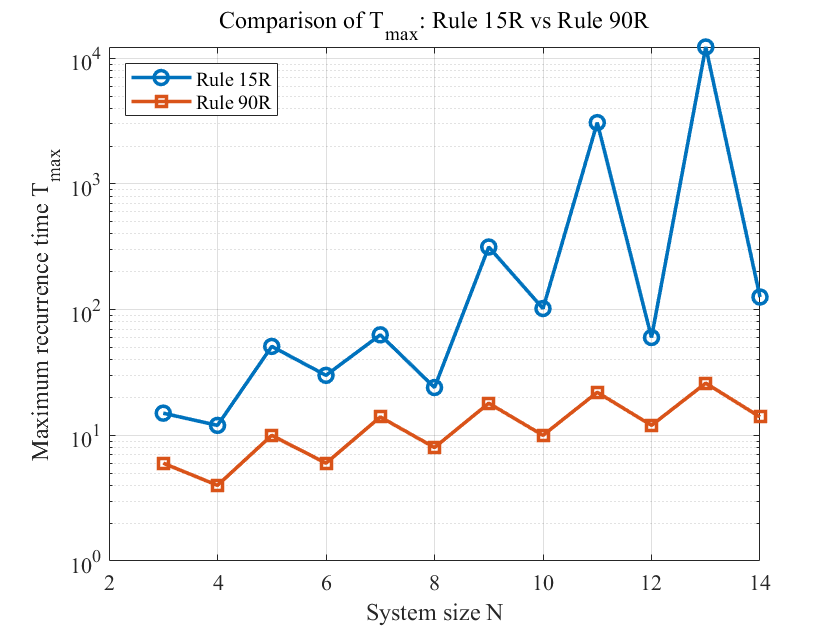
\includegraphics[width=0.48\textwidth]{image/Rule15R_90R_Tmax_Comparison.png}
    \caption{Rule 15R 与 Rule 90R 在周期边界条件下由完整双时间层相空间枚举得到的最大复现时间 $T_{\max}$。纵轴采用对数坐标，系统尺寸范围为 $N=3,\ldots,14$。}
    \label{fig:rule15_rule90_tmax}
\end{figure}

图~\ref{fig:rule15_rule90_tmax} 展示了 Rule 15R 与 Rule 90R 的最大复现时间随系统尺寸 $N$ 的变化。可以看到，二者虽然同属加性规则，但最大周期结构存在明显差异。Rule 15R 的 $T_{\max}$ 表现出强烈的尺寸依赖和锯齿状波动。特别是在若干奇数尺寸下，最大周期显著增大，例如 $N=9$ 时 $T_{\max}=315$，$N=11$ 时 $T_{\max}=3075$，$N=13$ 时进一步达到 $12291$；而在相邻偶数尺寸下，最大周期则明显下降，例如 $N=10$ 时 $T_{\max}=102$，$N=12$ 时为 $60$，$N=14$ 时为 $126$。这说明 Rule 15R 的周期结构并不服从简单的单调增长规律，而是受到系统长度、周期边界条件以及加性代数结构的共同影响。

相比之下，Rule 90R 的最大复现时间更加规则。在所计算的尺寸范围内，Rule 90R 呈现出清晰的奇偶依赖：当 $N$ 为偶数时，
\begin{equation}
    T_{\max}=N,
\end{equation}
而当 $N$ 为奇数时，
\begin{equation}
    T_{\max}=2N.
\end{equation}
例如，$N=8,10,12,14$ 时分别有 $T_{\max}=8,10,12,14$；而 $N=7,9,11,13$ 时分别有 $T_{\max}=14,18,22,26$。因此，Rule 90R 的最大周期并不是无波动的严格单调直线，而是具有奇偶交替结构，其上包络随 $N$ 近似线性增长。与 Rule 15R 相比，Rule 90R 的最大周期整体更短，说明其轨道扩展受到更强的代数限制。

\begin{figure}[htbp]
    \centering
    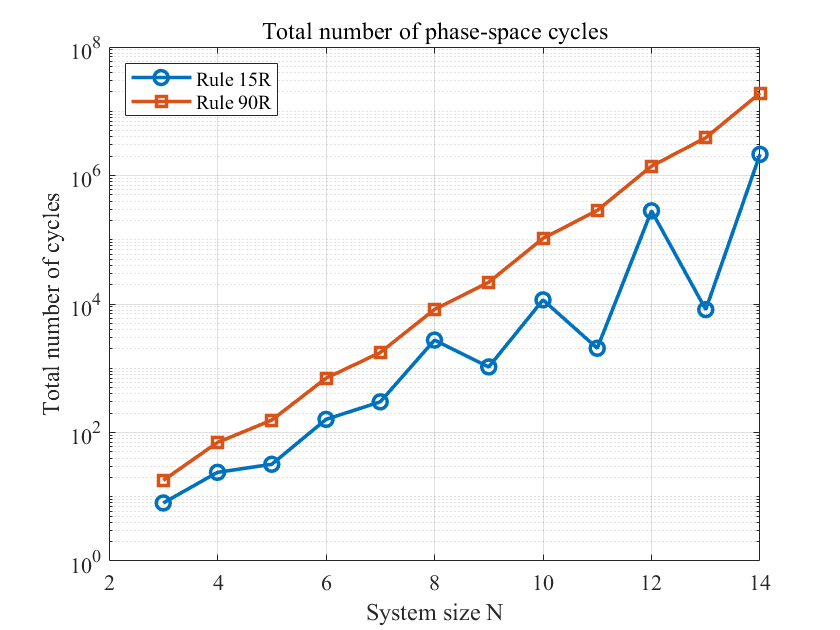
\includegraphics[width=0.48\textwidth]{image/Rule15R_90R_TotalCycles.png}
    \caption{Rule 15R 与 Rule 90R 的闭合轨道总数随系统尺寸 $N$ 的变化。闭合轨道总数反映有限可逆相空间被周期轨道分解的程度。纵轴采用对数坐标。}
    \label{fig:rule15_rule90_totalcycles}
\end{figure}

图~\ref{fig:rule15_rule90_totalcycles} 展示了两种加性规则下闭合轨道总数随系统尺寸的变化。随着 $N$ 增大，两种规则的闭合轨道总数整体上均快速增加，说明完整相空间被分解为越来越多的周期轨道，而不是由少数长轨道主导。Rule 90R 的闭合轨道数在多数尺寸下显著高于 Rule 15R，例如在 $N=14$ 时，Rule 90R 的闭合轨道数达到 $19175140$，而 Rule 15R 为 $2134948$。这表明 Rule 90R 的相空间被切分得更为细碎，系统轨道更倾向于形成大量短周期闭合环。

综合图~\ref{fig:rule15_rule90_tmax} 与图~\ref{fig:rule15_rule90_totalcycles} 可以看出，加性规则的相空间结构受到线性代数关系和周期边界条件的强烈影响。尽管完整相空间规模随 $N$ 按 $4^N$ 指数增长，Rule 15R 与 Rule 90R 的最大周期并未表现出与相空间规模相当的增长。Rule 15R 在若干尺寸下出现较长周期，但其增长具有明显的数论型波动；Rule 90R 则呈现出更强的规则性，其最大周期仅随系统尺寸线性增长。与此同时，闭合轨道总数的快速增加说明加性规则将相空间分割为大量相互独立的周期轨道。因此，这两类规则均表现出显著的代数约束，其最大轨道只能覆盖完整相空间中的极小部分，体现出加性 ERCA 的非随机轨道结构和有限尺寸效应。

\subsection{非线性规则 30R、75R 与 155R}

为了与加性规则进行对比，本文进一步研究了三种典型非线性规则 Rule 30R、Rule 75R 和 Rule 155R。与 Rule 15R 和 Rule 90R 不同，这些规则的局域更新函数不能简单表示为 $\mathrm{GF}(2)$ 上的线性或仿射线性函数，因此其相空间轨道通常不再受到同样强的线性代数约束。本文同样采用完整双时间层相空间枚举方法，对 $N=3,\ldots,14$ 的有限系统计算最大复现时间 $T_{\max}$ 以及闭合轨道总数。

\begin{figure}[htbp]
    \centering
    
\includegraphics[width=0.48\textwidth]{image/NonlinearTmaxExpFit.png}
    \caption{非线性规则 Rule 30R、Rule 75R 与 Rule 155R 在周期边界条件下由完整双时间层相空间枚举得到的最大复现时间 $T_{\max}$。纵轴采用对数坐标，黑色虚线表示三种规则平均趋势的指数拟合。}
    \label{fig:nonlinear_tmax}
\end{figure}

图~\ref{fig:nonlinear_tmax} 展示了三种非线性规则的最大复现时间随系统尺寸 $N$ 的变化。可以看到，在对数坐标下，Rule 30R、Rule 75R 和 Rule 155R 的 $T_{\max}$ 整体上随 $N$ 近似线性上升，说明其最大周期随系统尺寸呈现近似指数增长趋势。虽然不同规则之间存在有限尺寸波动，例如 Rule 155R 在部分尺寸下明显高于另外两条曲线，但三种规则的整体增长趋势较为一致。这与加性规则形成鲜明对比：Rule 90R 的最大周期仅随 $N$ 线性增长，而 Rule 15R 虽然存在较大的尺寸依赖波动，但其增长并不表现出稳定的指数趋势。

从具体数值上看，三种非线性规则在较大系统尺寸下均能产生远长于加性规则的周期轨道。例如在 $N=14$ 时，Rule 30R、Rule 75R 和 Rule 155R 的最大周期分别达到 $95052$、$66424$ 和 $126170$。这说明在缺乏简单线性叠加结构的情况下，非线性规则能够在有限相空间中形成更长的闭合轨道，反映出更强的相空间探索能力。

\begin{figure}[htbp]
    \centering
    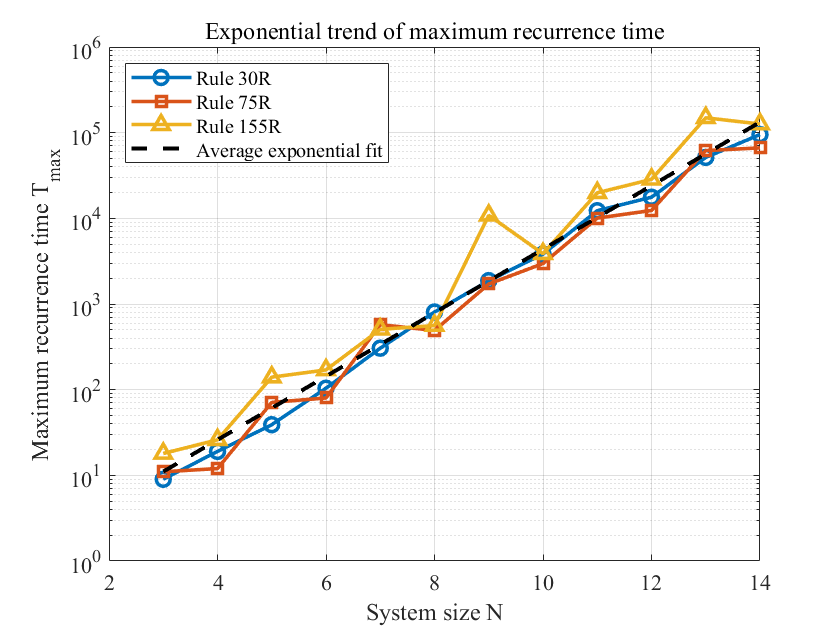
\includegraphics[width=0.48\textwidth]{image/NonlinearTotalCycles.png}
    \caption{非线性规则 Rule 30R、Rule 75R 与 Rule 155R 的闭合轨道总数随系统尺寸 $N$ 的变化。纵轴采用对数坐标。}
    \label{fig:nonlinear_totalcycles}
\end{figure}

图~\ref{fig:nonlinear_totalcycles} 给出了三种非线性规则对应的闭合轨道总数。随着系统尺寸增加，三种规则的闭合轨道数量整体上也快速增长，并在 $N=14$ 时达到 $10^4$ 数量级。其中 Rule 30R、Rule 75R 和 Rule 155R 在 $N=14$ 时的闭合轨道总数分别为 $32664$、$43204$ 和 $32026$。与 Rule 90R 在同一尺寸下超过 $10^7$ 的闭合轨道数量相比，非线性规则的轨道总数明显更少，但其最大周期显著更长。这表明非线性规则的相空间分解方式与加性规则不同：加性规则倾向于将相空间切分为大量短周期轨道，而非线性规则则更容易形成相对较长的闭合轨道。

需要强调的是，最大复现时间的指数增长并不等价于严格证明系统具有遍历性或热化性质。周期长度只能说明系统中存在较长的闭合轨道，并暗示非线性规则具有更强的相空间探索能力。若要进一步判断系统是否在统计意义上热化，还需要结合轨道长度分布、时间关联函数、扰动扩散以及粗粒化观测量的长期行为进行分析。因此，本文将 $T_{\max}$ 的指数增长视为非线性规则具有较强相空间探索能力的数值证据，而不将其单独作为严格遍历性的证明。

综上，二元 ERCA 的数值结果表明，加性规则与非线性规则在有限相空间分解方式上存在显著差异。加性规则的轨道结构受到线性代数关系和周期边界条件的强烈约束，表现为较短的最大周期和大量闭合轨道；非线性规则则能够产生随系统尺寸近似指数增长的长周期轨道，并且在同等系统尺寸下形成相对较少但更长的闭合轨道，显示出更强的相空间探索能力。需要再次强调的是，本节的复现时间和轨道总数分析属于相空间结构分析，而非严格热化证明。基于这一动机，下一节将把 ERCA 推广至平衡三进制情形，并进一步构造守恒量与热化判据。



%% ========================================================================
%% 拓展章节：平衡三进制的 ERCA
%% ========================================================================

\section{拓展：平衡三进制的 ERCA}

本节首先构造平衡三进制 ERCA，并在此基础上分析其规则对称性、加性守恒量结构以及热化倾向。

目前研究的元胞自动机全部是具有两个状态的，这可能是因为现代计算机都使用二进制导致的。但是，如果我们是将其作为一种物理系统来研究，那么每个格点的状态数似乎不一定必须为两个。下面我们介绍一种曾在苏联计算机 Setun 中使用的平衡三进制，并构建相应的 ERCA 规则\cite{Setun,VICHNIAC198496}。

\subsection{引入}

平衡三进制的每一位有三个状态，即 $0$，$1$ 和 $-1$（在写数字时常用 $\mathrm{T}$ 表示）。对于一个用该进制表示的数：
\begin{equation}
a_n a_{n-1} \dots a_2 a_1, \quad a_i = -1, 0, 1
\end{equation}
其表示的值为：
\begin{equation}
\sum_{i=1}^n a_i 3^{i-1}
\end{equation}
由此可见，平衡三进制能够不带整体符号地同时表示正数和负数。比如 $1\mathrm{T}$ 可表示十进制中的 $2$，则 $\mathrm{T}1$ 就可以表示十进制中的 $-2$。

对于 ERCA 的规则表达式：
\begin{equation}
    \begin{aligned}
        & \sigma_i^{t+1} = f(\sigma_{i-1}^t, \sigma_{i}^t, \sigma_{i+1}^t) \otimes r_i^t\\
        & r_i^{t+1} = \sigma_i^t \\
    \end{aligned}
    \label{rule}
\end{equation}
需要重新定义的是原二进制中的异或运算“$\otimes$”。我们假设这样的运算和异或一样满足交换律。而且，为了满足规则的可逆性质，这样的运算必须满足：如果 $a \otimes b = c$，那么 $a \otimes c = b$。通过列举所有规则，我们找到如下三个符合这种要求的规则：

\begin{figure}[htbp]
\centering
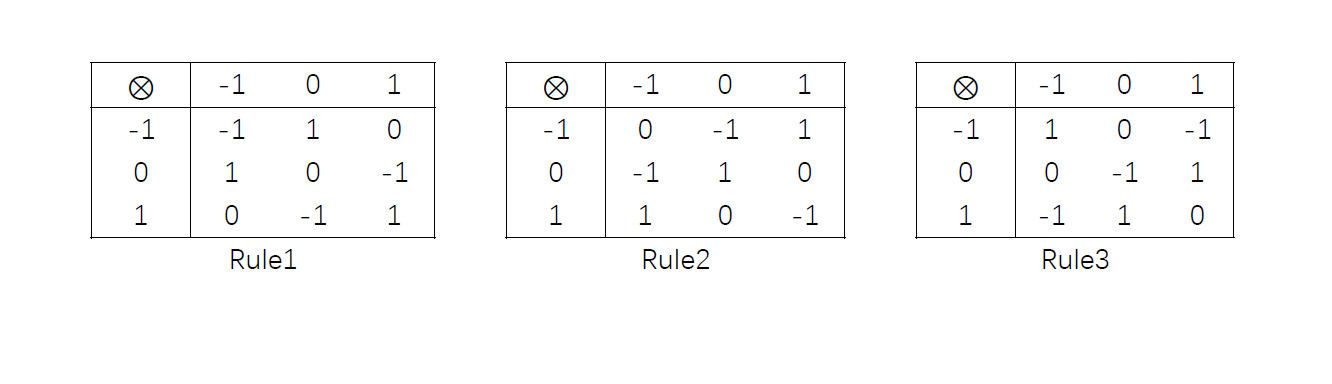
\includegraphics[width=0.5\textwidth]{image/3XORS.png} % 请在此处放置平衡三进制的三种运算规则图片
\caption{\label{fig:ternary_operators} 可用作平衡三进制 ERCA 的三种 $\otimes$ 运算规则。}
\end{figure}

三种$ \otimes $运算在可逆性要求下具有相似的代数结构\cite{Latin}，因此本文固定选取第一种运算表作为研究对象。不同 $\otimes$ 表之间是否严格给出相同的动力学分类，需要结合 f 的变换关系进一步检验。本文后续结果应理解为在固定该$ \otimes $表下得到的分类结果。

\subsection{对称性}

很显然，三元 ERCA 可能的规则数目和二元相比是远远多的。鉴于 $f(\sigma_{i-1}^t, \sigma_{i}^t, \sigma_{i+1}^t)$ 有三种可能取值和三个具有三种取值的自变量，那么一共应有 $3^{3^3} = 3^{27} \approx 7 \times 10^{12}$ 种不同的规则。这是一个非常大的数目，较难以沿用研究二元 ERCA 的方法，对每个规则进行遍历研究。
我们尝试使用类似的方法对三元ERCA的对称性进行分析。在以下的运算中，我们将简记：
\begin{equation}f(\sigma_{i-1}^t, \sigma_{i}^t, \sigma_{i+1}^t) = f(\mu, \nu, \kappa)\end{equation}

为之后讨论做铺垫，我们将首先介绍一下群相关的定义\cite{group}：

设 $G$ 是一些元素（操作）的集合，记为 $G = \{\cdots, g, \cdots\}$，在 $G$ 中定义了乘运算，如果 $G$ 中元素对这种运算满足下面四个条件：
\begin{enumerate}
    \item \textbf{封闭性}：$\forall$ 两个元素（操作）的乘积仍属于这类元素（操作）的集合；
    \item \textbf{结合律}：对 $\forall$ 三个元素（操作）$f, g, h$，有 $(fg)h = f(gh)$；
    \item \textbf{单位元}：有唯一单位元素 $e$，使得对 $\forall f \in G$，有 $ef = fe = f$；
    \item \textbf{逆元}：对 $\forall f \in G$，存在且唯一存在 $f^{-1} \in G$，使 $f^{-1}f = ff^{-1} = e$。
\end{enumerate}
则称 $G$ 为一个\textbf{群}。

\textbf{子群}：设 $G$ 是一个群，$H$ 是 $G$ 的一个子集，如果 $H$ 中的元素在 $G$ 中的乘法运算下也构成一个群，则称 $H$ 是 $G$ 的一个\textbf{子群}。

基于上方已经构建出来的可逆运算，三元ERCA构成了一个对称操作群:$G = S_3 \times Z_2$。其中，$S_3$ 群代表的是轮换操作：
\begin{align}
    e:f(\mu,\nu,\kappa) &\to f(\mu,\nu,\kappa) \nonumber \\
    C^1 :f(\mu,\nu,\kappa) &\to f(\nu,\mu,\kappa) \nonumber \\
    C^2 :f(\mu,\nu,\kappa) &\to f(\mu,\kappa,\nu) \nonumber \\
    C^3 :f(\mu,\nu,\kappa) &\to f(\kappa,\nu,\mu) \nonumber \\
    C^4 :f(\mu,\nu,\kappa) &\to f(\nu,\kappa,\mu) \nonumber \\
    C^5 :f(\mu,\nu,\kappa) &\to f(\kappa,\mu,\nu) 
\end{align}
共有六种不同的轮换操作。需要强调的是，本文此处的$S_3$作用在局域规则的三个输入位置上，即交换$ μ,ν,κ$ 的排列顺序，而不是直接置换状态值 $−1,0,1$ 。而$Z_2$ 群代表的是状态变换操作：
\begin{align}
    e: f(\mu,\nu,\kappa) &\to f(\mu,\nu,\kappa) \nonumber \\
    S: f(\mu,\nu,\kappa) &\to -f(-\mu, -\nu, -\kappa) 
\end{align}
有两种不同的状态操作。因此，三元 ERCA 的对称操作总共有 $6 \times 2 = 12$ 个。
在这$12$个操作下，若$f$的对应关系不发生改变，那么我们就认为这些规则是等价的。
这远多于二元 ERCA 的 $4$ 种操作。这样，每个等价类中最多也就可能有 $12$ 个成员。如何计算等价类的数目？在研究二元 ERCA 时，研究者可以计算所有 $256$ 个规则经三种对称操作后变为了哪种规则，并划分出所有的 $88$ 个等价类。但由于三元的规则数目太多，就无法遍历计算。我们需要发展一种组合数学的方法，从而不需要考察每一个规则就能计算出等价类的数目。

在具体分析实际操作下规则的等价关系之前，我们先来分析一下这些操作的代数结构。首先，轮换操作 $S_3$ 群是非阿贝尔群，状态变换操作 $Z_2$ 群是阿贝尔群。两者的乘积群 $G$ 也是非阿贝尔群。
这指引我们去分析三元ERCA的$G$群各个子群，从而分析这些子群变换下的等价类。
\begin{enumerate}
    \item 一阶子群：$H_1 = (e)$. 该子群只有一个元素，即恒等操作。对于任何规则 $f$，我们都有 $ef = fe = f$，因此每个规则都在该子群下具有不变性。
    \item 二阶子群：
    \begin{equation*}
        \begin{aligned}
        H_{2A}^{(i)} &= \{e, C^i\}, \quad i = 1, 2, 3  \\
        H_{2B} &= \{e, S\}  \\
        H_{2C}^{(i)} &= \{e, SC^i\}, \quad i = 1, 2, 3 
    \end{aligned}
    \end{equation*}
    其中 $H_2^{1(i)}$ 是三种轮换操作中的一种，$H_2^2$ 是状态变换操作，$H_2^{3(i)}$ 是状态变换和轮换的联合操作。
    \item 三阶子群：$H_3 = \{e, C^4 , C^5\}$. 
    \item 四阶子群：$H_4^{i} = \{e, S, C^i, SC^i\}, \quad i = 1, 2, 3$. 
    \item 六阶子群：
    \begin{equation*}
        \begin{aligned}
        H_{6A} &= \{e, C^1, C^2, C^3, C^4, C^5\}  \\
        H_{6B} &= \{e, C^4, C^5, S, SC^4, SC^5\} \\
        H_{6C} &= \{e, C^4, C^5, SC^1, SC^2, SC^3\}
        \end{aligned}
    \end{equation*}
    其中 $H_6^1$ 是轮换操作的子群即$S_3$ ， 而$H_6^2$ 和 $H_6^3$ 是状态变换和轮换的联合操作。
    \item 十二阶子群：$G = S_3 \times Z_2$. 该子群包含了所有的对称操作。
\end{enumerate}
如果我们认为每个规则 $f$ 都是一个 $3^3$ 维空间中的一个点，那么这些对称操作就相当于在这个空间中对这些点进行变换。对于某个规则 $f$，如果它在某个子群 $H$ 下具有不变性，那么我们就可以说这个规则在该子群下是对称的。对于一个规则 $f$，如果它在某个子群 $H$ 下具有不变性，那么它在该子群的所有元素下都具有不变性。因此，我们可以通过分析规则在不同子群下的对称性，来划分出不同的等价类。

若规则在子群$H$下不变，用数学表述即为：
\begin{equation}
    h \cdot f = f , \quad \forall h \in H
\end{equation}
设群$H$作用在集合$X$上，那么对于$\forall x \in X$，定义\textbf{轨道}是：
\begin{equation}
    \text{Orb}(x) = {h \cdot x | h \in H}
\end{equation}
即从$X$出发，经过$H$中所有元素作用后能到达的所有点的集合。
轨道即是等价类，所以 $X$可以被划分成若干个互不相交的轨道。
对称规则数在不计入更高的对称性的情况下，对称规则数的个数$N = 3^{\text{轨道数}}$。$3$是因为输出有三个取值：${-1 , 0 ,1}$。

\begin{table}[htbp]
\caption{\label{tab:orbit_count} 三元 ERCA 的各个子群的轨道数目和对称规则数}
\begin{ruledtabular}
\begin{tabular}{lcc}
子群 & 轨道数目 & 对称规则数$N$\\
\colrule
$H_1$ & 27 & $3^{27}$ \\
$H_{2A}^{(i)}$ & 18 & $3^{18}$ \\
$H_{2B}^2$ & 14 & $3^{14}$ \\
$H_{2C}^{(i)}$ & 15 & $3^{15}$ \\
$H_3$ & 11 & $3^{11}$ \\
$H_4^{i}$ & 10 & $3^{10}$ \\
$H_{6A}$ & 10 & $3^{10}$ \\
$H_{6B}$ & 6 & $3^{6}$ \\
$H_{6C}$ & 7 & $3^{7}$ \\
$G$ & 6 & $3^{6}$ \\
\end{tabular}
\end{ruledtabular}
\end{table}

可以发现对于上面子群，有 $H_1 \in G$。这会导致在计算等价类计数时出现重复计数的问题，所以我们需要“恰好以$H$为最大不变子群”的规则数量，即满足在 $H$ 下具有不变性，但在任何包含 $H$ 的更大子群下都不具有不变性的规则数目。
这个数目我们称为 $N_H$，可以通过容斥原理计算出来：
\begin{equation}
    N_H = N - \sum_{H' \supset H} N_{H'}
\end{equation}
其中 $N$ 是在 $H$ 下具有不变性的规则数目，$\sum_{H' \supset H} N_{H'}$ 是在包含 $H$ 的更大子群下具有不变性的规则数目的总和。
通过一系列计算，我们可以得到修正之后的表格~\ref{tab:corrected}，其中 $N_i$ 是仅具有该子群不变性的规则数目。
\begin{table}[htp]
\caption{\label{tab:corrected} 三元 ERCA 的各个子群的仅具有该子群不变性的规则数目}
\begin{ruledtabular}
\begin{tabular}{lc}
子群 & 仅具有该子群不变性的规则数 $N_i$ \\
\colrule
$H_1$ & $3^{27} - 3^{19} - 3^{16} - 3^{14} + 2 \cdot 3^{11} + 3^{7} +3^{6}$ \\
$H_{2A}^{(i)}$ & $3^{18} - 2 \cdot 3^{10}  + 3^{6}$\\
$H_{2B}^2$ & $3^{14} - 3^{11} + 3^{7} - 3^{6}$\\
$H_{2C}^{(i)}$ & $3^{15} - 3^{10} - 3^{7} + 3^{6}$ \\
$H_3$ & $3^{11}- 3^{10} - 3^{7} + 3^{6}$ \\
$H_4^{i}$ & $3^{10} - 3^{6}$ \\
$H_{6A}$ &  $3^{10} - 3^{6}$ \\
$H_{6B}$ &  0 \\
$H_{6C}$ &  $3^{7} - 3^{6}$ \\
$G$ &  $3^{6}$ \\
\end{tabular}
\end{ruledtabular}
\end{table}

$N_1$其实对应的就是不存在任何对称性的规则数目。$H_{6B}$的$N$为$0$是由于$H_{6B}$的所有对称规则都被更大的子群覆盖这是由于子群之间的包含关系。当然，在计算等价类数目时，我们还需要考虑每个等价类中规则的数量。对于具有 $H$ 不变性的规则来说，每个等价类（轨道）的大小为$\dfrac{|G|}{|H|}$。
其中$|G|$为$G$的阶数，$|H|$为$H$的阶数，即$H$中元素的数量。对于每个子群$H$，我们可以计算出其阶数，然后根据等价类的大小来计算每个子群下的等价类数量。总等价类个数为：
\begin{equation}
    \begin{aligned}
    &n = \sum_i \frac{N_i\,|H_i|}{|G|} \\
    & = \frac{1}{12}(3^{27} + 3^{19} + 3^{16} + 3^{14} +2 \cdot 3^{11} + 2 \cdot 3^{6})\\
    & = 635567327658 \approx 6.36 \times 10^{11}
    \end{aligned}
\end{equation}


这就是如果我们要对每个等价类逐一考察所需要面对的数据规模：
$10^{11}$ 数量级。通过引入对称群
\[
    G=S_3\times Z_2,
\]
我们可以将大量表面上不同的三值局域规则归入同一等价类。
这些等价规则之间可以通过输入位置置换与状态取反相互转化，
因而在相应的变量变换下具有相同的相空间结构和轨道分解方式。
因此，本文后续只需对每个等价类的代表规则进行分析，
即可刻画该类规则共同的动力学性质。



\subsection{三元 ERCA 的动力学特征}
由于三元ERCA仍然满足二元的可逆结构，我们同样期待他满足与二元ERCA类似的动力学特征。同样，我们期望其同样满足热化，接下来我们将分析一下可热化的条件。
我们定义三元ERCA的\textbf{热化条件}为：当系统尺寸趋于无穷大时，系统的微观轨道能够遍历整个相空间，即系统具有完全的各态历经性（Ergodicity）。在二元ERCA中，我们已经知道，具有局域守恒律的规则（如90R）会导致系统的微观轨道被锁死在局部相空间碎片中，从而破坏了热化条件。而对于三元ERCA，我们同样需要分析其是否存在类似的局域守恒律，以及这些守恒律如何影响系统的遍历性。
通过对三元ERCA的规则进行分析，我们发现，某些规则确实存在局域守恒律，这些守恒律会导致系统的微观轨道被限制在某些特定的相空间区域内，从而破坏了热化条件。另一方面，也存在一些规则没有任何局域守恒律，这些规则的微观轨道能够遍历整个相空间，从而满足热化条件。因此，三元ERCA的热化条件同样取决于其规则是否存在局域守恒律。
总之，由于三元ERCA的动力学特征与二元ERCA有着相似的结构，热化条件同样取决于规则是否存在局域守恒律。

定义一个可加性的守恒量如下：
\begin{equation}
    \Phi = \sum_i F(\sigma_i^t , r_i^t , \sigma_{i+1}^t , r_{i+1}^t)
\end{equation}

其中$F$是一个全局函数，如果对于某个规则来说，存在一个非平凡的$F$使得$\Phi$在演化过程中保持不变，那么我们就说这个规则具有一个可加性的守恒量。即在规则的一次全局更新下，$\Phi(t+1)=\Phi(t)$。

体系的配分函数可以用来分析系统的热化行为。对于三元ERCA，我们可以定义一个配分函数来描述系统在不同状态下的统计权重。通过计算配分函数，我们可以得到系统的热力学性质，如自由能、熵等，从而进一步分析系统的热化行为。配分函数的定义式如下：
\begin{equation}
    \begin{aligned}
    &Z = \sum exp[-\beta \Phi] \\
    &= \sum_{\sigma_1 , r_1} \cdots \sum_{\sigma_n , r_n} \prod_{i} exp[-\beta F(\sigma_i^t , r_i^t , \sigma_{i+1}^t , r_{i+1}^t)]\\
    \end{aligned}
\end{equation}

$F$总计$3^4=81$种输入。对于任意格点$i$，定义\textbf{局域流}如下：
\begin{equation}
    F(\sigma_i^{t+1} , r_i^{t+1} , \sigma_{i+1}^{t+1} , r_{i+1}^{t+1})-F(\sigma_i^t , r_i^t , \sigma_{i+1}^t , r_{i+1}^t)= J_i - J_{i+1}
\end{equation}
若对于所有的格点$i$都满足这个关系，那么体系可以天然满足$\sum_i (J_{i+1}-J_{i}) = 0$，进一步我们可以得到$\Phi(t+1)=\Phi(t)$。这预示着若体系可以解耦成局域流的存在，则必会存在一个相应的加性守恒量。

但若继续沿用Shinji Takesue\cite{shinjin}关于对所有的F进行穷举的方式，数据集太过庞大。我们尝试采用约束矩阵的方法求解。
对长度$L$的环，枚举所有$3^{2L}$个初始构型。对每个构型，进行一步演化，要求$\Phi(t+1) - \Phi(t) = 0$，得到关于$\mathbf{F} \in \mathbb{R}^{81}$的线性齐次方程。收集所有$3^{2L}$个方程，构成约束矩阵$M_f$（$3^{2L} \times 81$），守恒条件为：
\begin{equation}
    M_f \cdot \mathbf{F} = 0
\end{equation}
通过奇异值分解（SVD）计算零空间维度$d = 81 - \operatorname{rank}(M_f)$。数值容差取$10^{-10}$，前54-72个奇异值显著大于零（$\sim 1-15$），其余接近机器精度（$\sim 10^{-15}$）。由该定义，我们可以得知，$d$的大小跟一维环的长度$L$无关。

在接下来的计算中，我们使用的$\otimes$形式如下：
\begin{equation}
\otimes = \begin{pmatrix}
-1 & 1 & 0 \\
1 & 0 & -1 \\
0 & -1 & 1
\end{pmatrix}
\end{equation}
其中行索引对应$a$（取$-1,0,1$），列索引对应$b$（取$-1,0,1$）。
正如我们前面提到的：$\otimes$ 的选取并不会导致它们在相空间层面产生完全不同的轨道划分。热化/非热化的分类在三个表中高度一致，两两之间的Jaccard相似度高达0.96\cite{jaccard}，而这两两之间的差异可能来自离散规则空间中标号变化导致的边界效应。
这在一方面，表示了三个$\otimes$的源于同一个代数空间。另一方面，表明热化是$\{f, \otimes\}$组合的属性，而非$f$的固有属性。

\subsubsection{F的零空间}
我们先来简单分析一下$F$的性质。若有一个良好函数$F$使得：
\begin{equation}
    F_J (\sigma_i , r_i , \sigma_{i+1} , r_{i+1}) = J(\sigma_i , r_i) - J(\sigma_{i+1} , r_{i+1})
    \label{F_J}
\end{equation}
这表明$F$被完全解耦，这会导致$\sum_i F \equiv 0$。而这对于所有的规则都成立，自然而然，这种特殊的$F_J$属于$F$的零空间。

$J$总共有$3^2=9$组，但这9个$J$中线性独立项只有8个。
\begin{equation}
    J(\sigma_i , r_i) = \sum_{a , b \in \{-1 ,0 ,1\}} J(a , b)\delta_{\sigma_i = a , r_i = b}
\end{equation}
$J(a,b)$为$J(\sigma_i , r_i)$在$(a,b)$上的取值。
代入\ref{F_J}式有：
\begin{equation}
    \begin{aligned}
            & F_J (\sigma_i , r_i , \sigma_{i+1} , r_{i+1}) \\
            & = \sum_{a , b } J(a , b) \delta_{\sigma_i = a , r_i = b} - \sum_{a , b} J(a , b)\delta_{\sigma_{i+1} = a , r_{i+1} = b} \\
            & = \sum_{a , b } J(a , b) (\delta_{\sigma_i = a , r_i = b}-\delta_{\sigma_{i+1} = a , r_{i+1} = b}) \\
            & = \sum_{a , b } J(a , b) F_{a,b}(\sigma_i , r_i , \sigma_{i+1} , r_{i+1})
    \end{aligned}
\end{equation}
我们可以把基取做：$F_{a,b}(\sigma_i , r_i , \sigma_{i+1} , r_{i+1})\equiv \delta_{\sigma_i = a , r_i = b}-\delta_{\sigma_{i+1} = a , r_{i+1} = b}$。
这组基自然满足：
\begin{equation}
    \sum_{a,b \in \{-1 ,0 ,1\}}F_{a,b} = 0
\end{equation}
这9个基向量线性相关，零空间$d=8$。再加上$F\equiv 1$引入的1维（$F\equiv -1$与$F\equiv 1$等价）。则有$d=9$维不依赖于f选择的F的零空间，称为$F$的平凡零空间。

那么减去这9维的平凡零空间后，$d-9$为非平凡动力学守恒量的维数。在经典力学中，Kolmogorov \cite{BFb0021737}提出的 KAM 理论指出，可积系统的准周期运动在微小扰动下得以保持，轨道被约束在不变环面上，无法遍历整个相空间。由此，我们可以假设：
$d = 9$意味着无额外守恒量，系统可能热化；$d > 9$意味着存在额外守恒量，相空间被约束在低维子流形上，系统确定非热化。

由于约束矩阵的每一行对应一个局域构型的守恒条件，而所有可能的局域构型已在枚举中全部包含，因此 $L$的增加只增加方程的数目而不增加未知数的维度，零空间维数$d$与$L$无关。

\subsection{对称性和热化条件}
根据\ref{tab:corrected}的内容，我们对各个对称性进行分析。
\begin{table}[h]
\centering
\caption{各对称类在不同采样数下的热化比例（$d=9$ 的规则占比）}
\label{tab:thermalization_sampling}
\begin{tabular}{lccccc}
\toprule
对称类 & $n=30$ & $n=50$ & $n=100$ & $n=500$ & $n=1000$ \\
\midrule
$H_1$ & 100.0\% & 96.0\% & 97.0\% & 98.0\% & 98.1\% \\
$H_{2A}$ & 100.0\% & 100.0\% & 99.0\% & 98.0\% & 98.4\% \\
$H_{2B}$ & 100.0\% & 86.0\% & 90.0\% & 90.4\% & 90.4\% \\
$H_{2C}$ & 96.7\% & 98.0\% & 96.0\% & 98.0\% & 96.5\% \\
$H_3$ & 0.0\% & 0.0\% & 0.0\% & 0.0\% & 0.0\% \\
$H_4$ & 93.3\% & 88.0\% & 86.0\% & 89.6\% & 86.3\% \\
$H_{6A}$ & 0.0\% & 0.0\% & 0.0\% & 0.0\% & 0.0\% \\
$H_{6B}$ & 0.0\% & 0.0\% & 0.0\% & 0.0\% & 0.0\% \\
$H_{6C}$ & 0.0\% & 0.0\% & 0.0\% & 0.0\% & 0.0\% \\
$G$ & 0.0\% & 0.0\% & 0.0\% & 0.0\% & 0.0\% \\
\bottomrule
\end{tabular}
\end{table}

\begin{figure}[H]
\centering
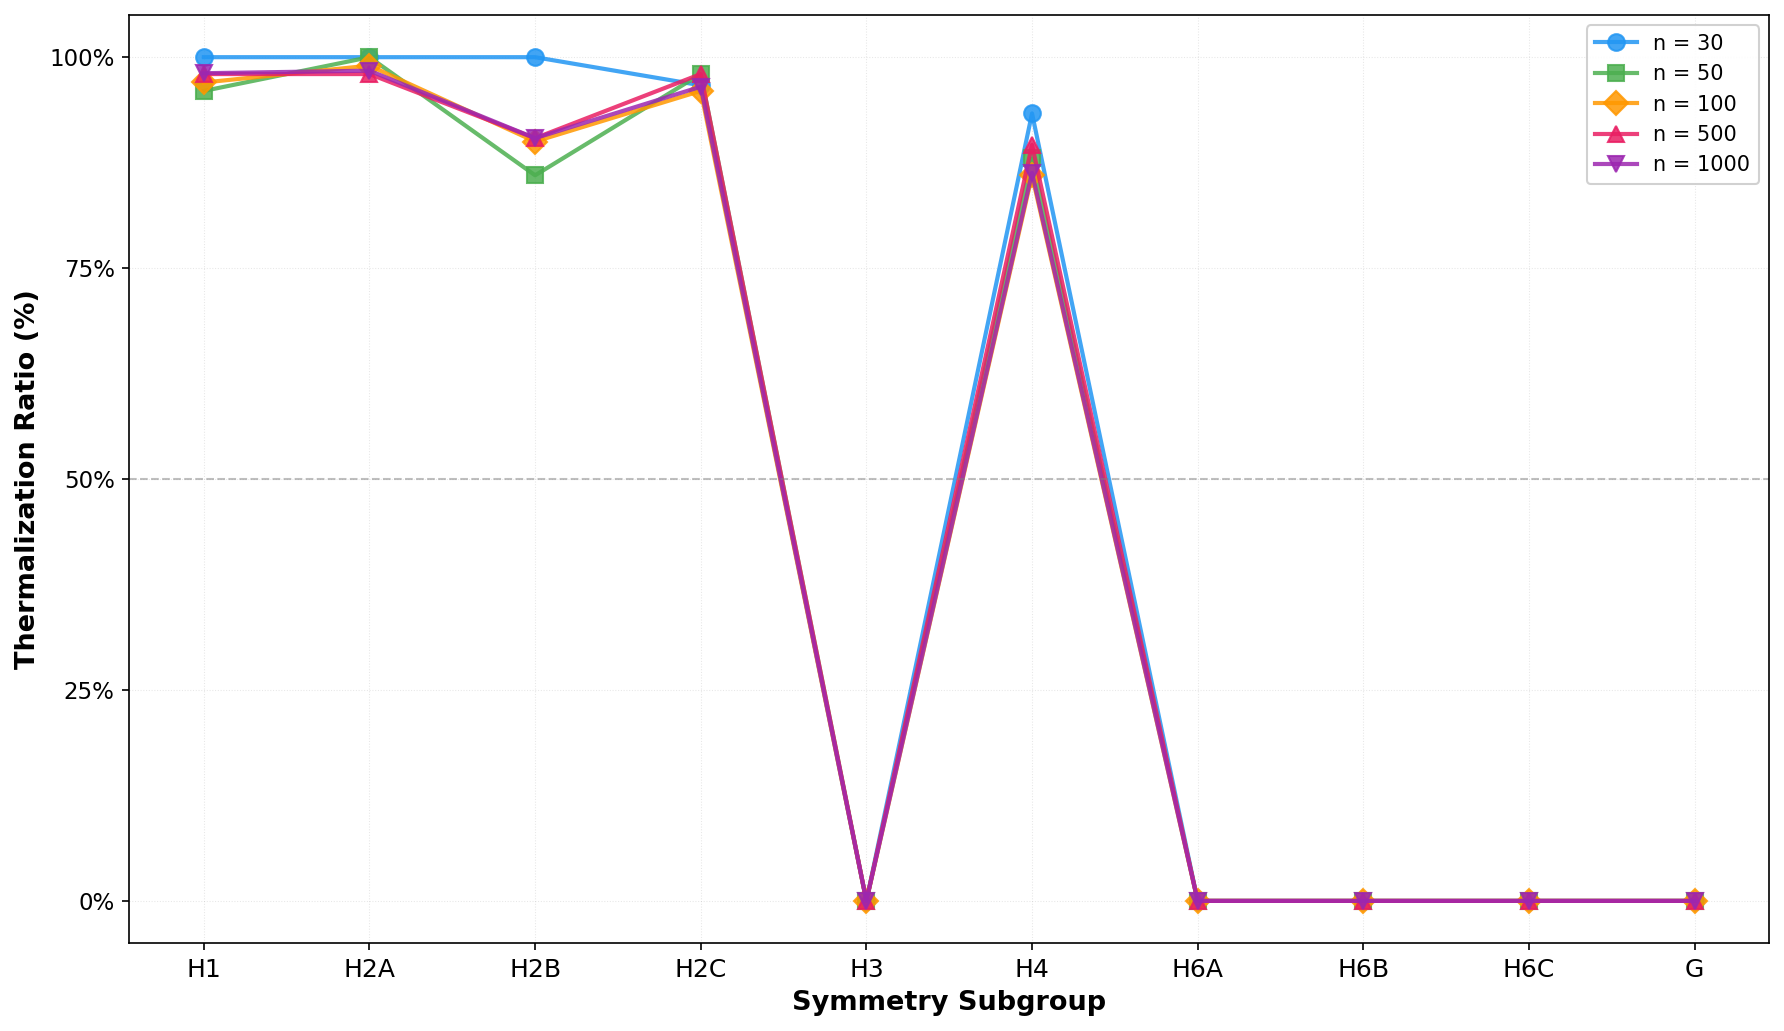
\includegraphics[width=0.45\textwidth]{image/thermalization_vs_symmetry.png} 
\caption{\label{fig:thermalization_vs_symmetry} 各对称类在不同采样数下的热化比例。}
\end{figure}

所有具有三元轮换性的$f$均不满足热化条件，发生\textbf{可热化-热化相变}。这个也是易于分析的。由于三元轮换对称性：$f(\nu , \mu , \kappa) = f(\kappa , \nu , \mu) = f(\mu , \kappa , \nu)$
在群$H_3$的影响下，定义域$\{-1,0,1\}^3$被划分为11条互不相交的轨道，而这种三轮换对称性强制$f$在 11 个轨道上取常值，
导致更新规则中的"耦合"减弱。具体而言，在$\sigma_i^{t+1} = f(\sigma_{i-1}^t, \sigma_{i}^t, \sigma_{i+1}^t) \otimes r_i^t$中，
$f$对其三个输入的对称化使得某些线性约束变得冗余。

在数学上，三轮换对称性导致$M_f$的行向量之间出现额外的线性关系。这些线性关系减少了独立方程的数量，从而降低了秩，增加了零空间维度。
三轮换对称性约束了$f$的结构，使得某些局域模式在演化中保持不变。

三轮换对称性破坏热化的机制在二元和三元的 ERCA 中是普适的。这不是三元系统特有的现象，而是 ERCA 的一般性质。
在二元ERCA中，三轮换对称性会显著降低轨道长度，从而将系统局域在部分小的像空间内。两者的区别在于三元ERCA由于相空间更大，非热化轨道长度仍然是一个较大的量，但相较于热化的轨道长度更小。
所以我们认为：
在形如式\ref{rule}的n元ERCA构造中，三元轮换对称性破坏系统可热化是普适的。

\begin{figure}[H]
\centering
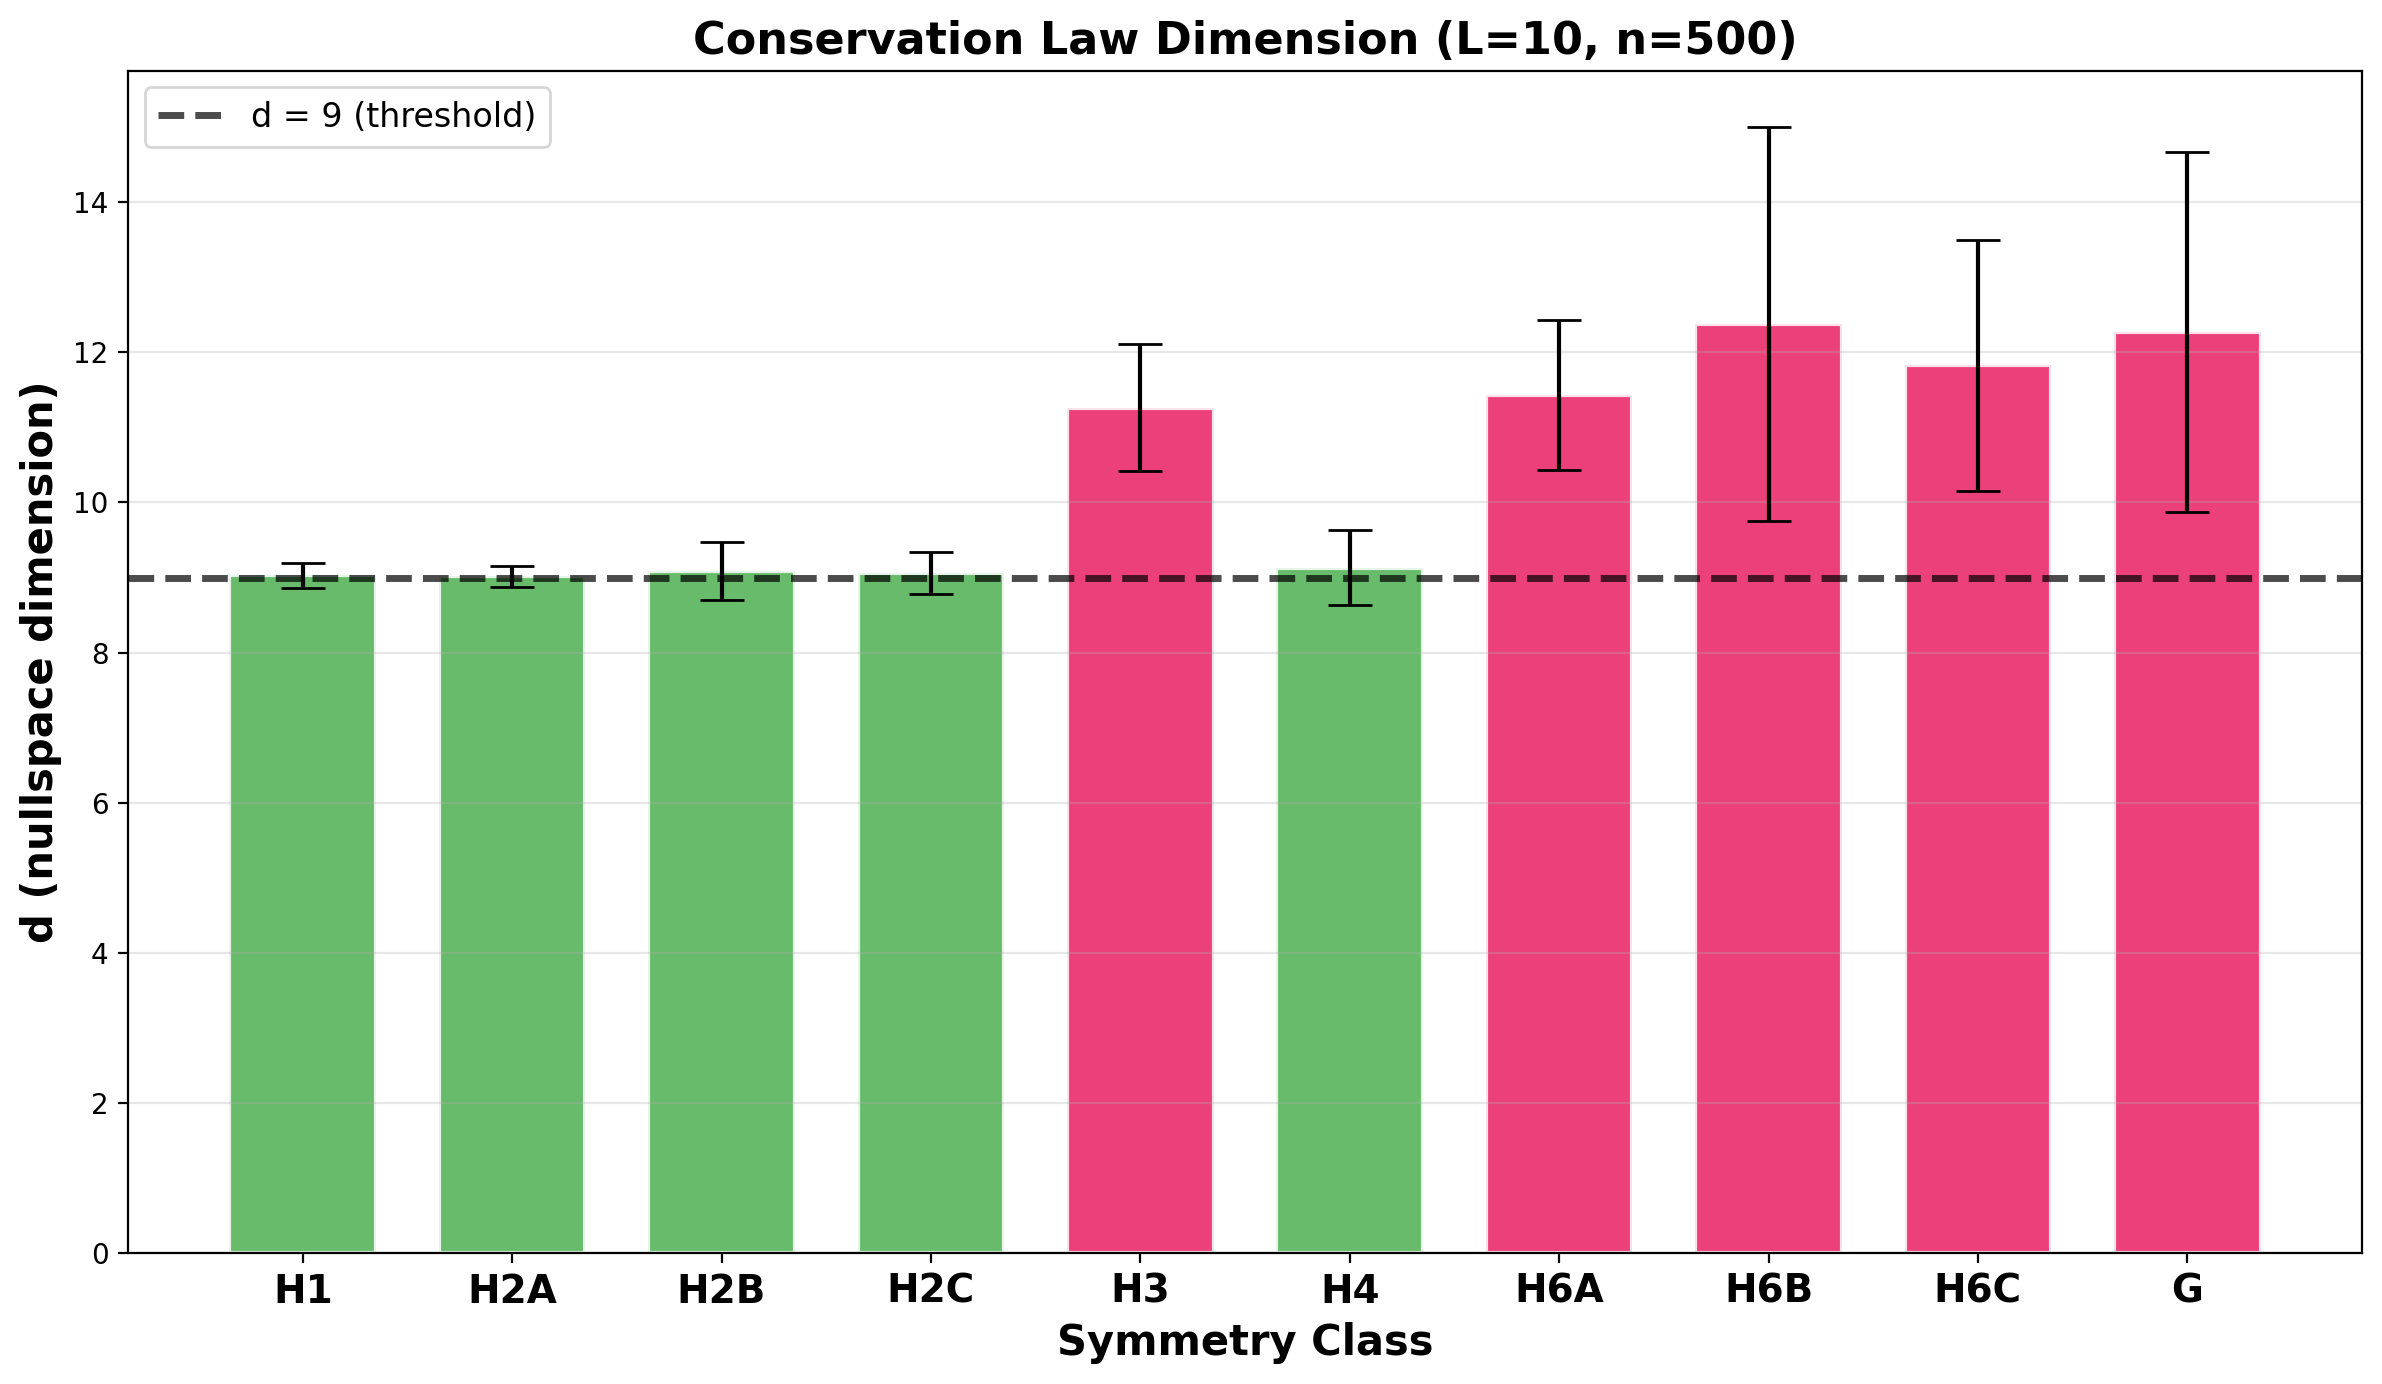
\includegraphics[width=0.45\textwidth]{image/fig1_d_value.png} 
\caption{\label{fig:d_symmetry} 各对称类的守恒量维度$d$。绿色柱表示热化类（$d \approx 9$），红色柱表示非热化类（$d > 9$）。黑色虚线标记$d=9$的热化阈值。误差棒为标准差。}
\end{figure}

由图\ref{fig:d_symmetry}中，我们可以发现具有三元轮换对称性的$f$最低维数为11，但目前没有得出一个相对完美的理论解释。

\subsection{热化的进一步讨论}
在前面我们提到$d=9$是热化的判定标准。在这一部分，我们将关注于具体的热化性。在接下来的讨论中，我们将使用$T01101001T101010010110T0001$（具体规则见\ref{tab:ternary_rule}）作为$d=9$的可热化的例子，$f \equiv 1$为$d=27$的例子作为对照。

\begin{figure}[H]
\centering
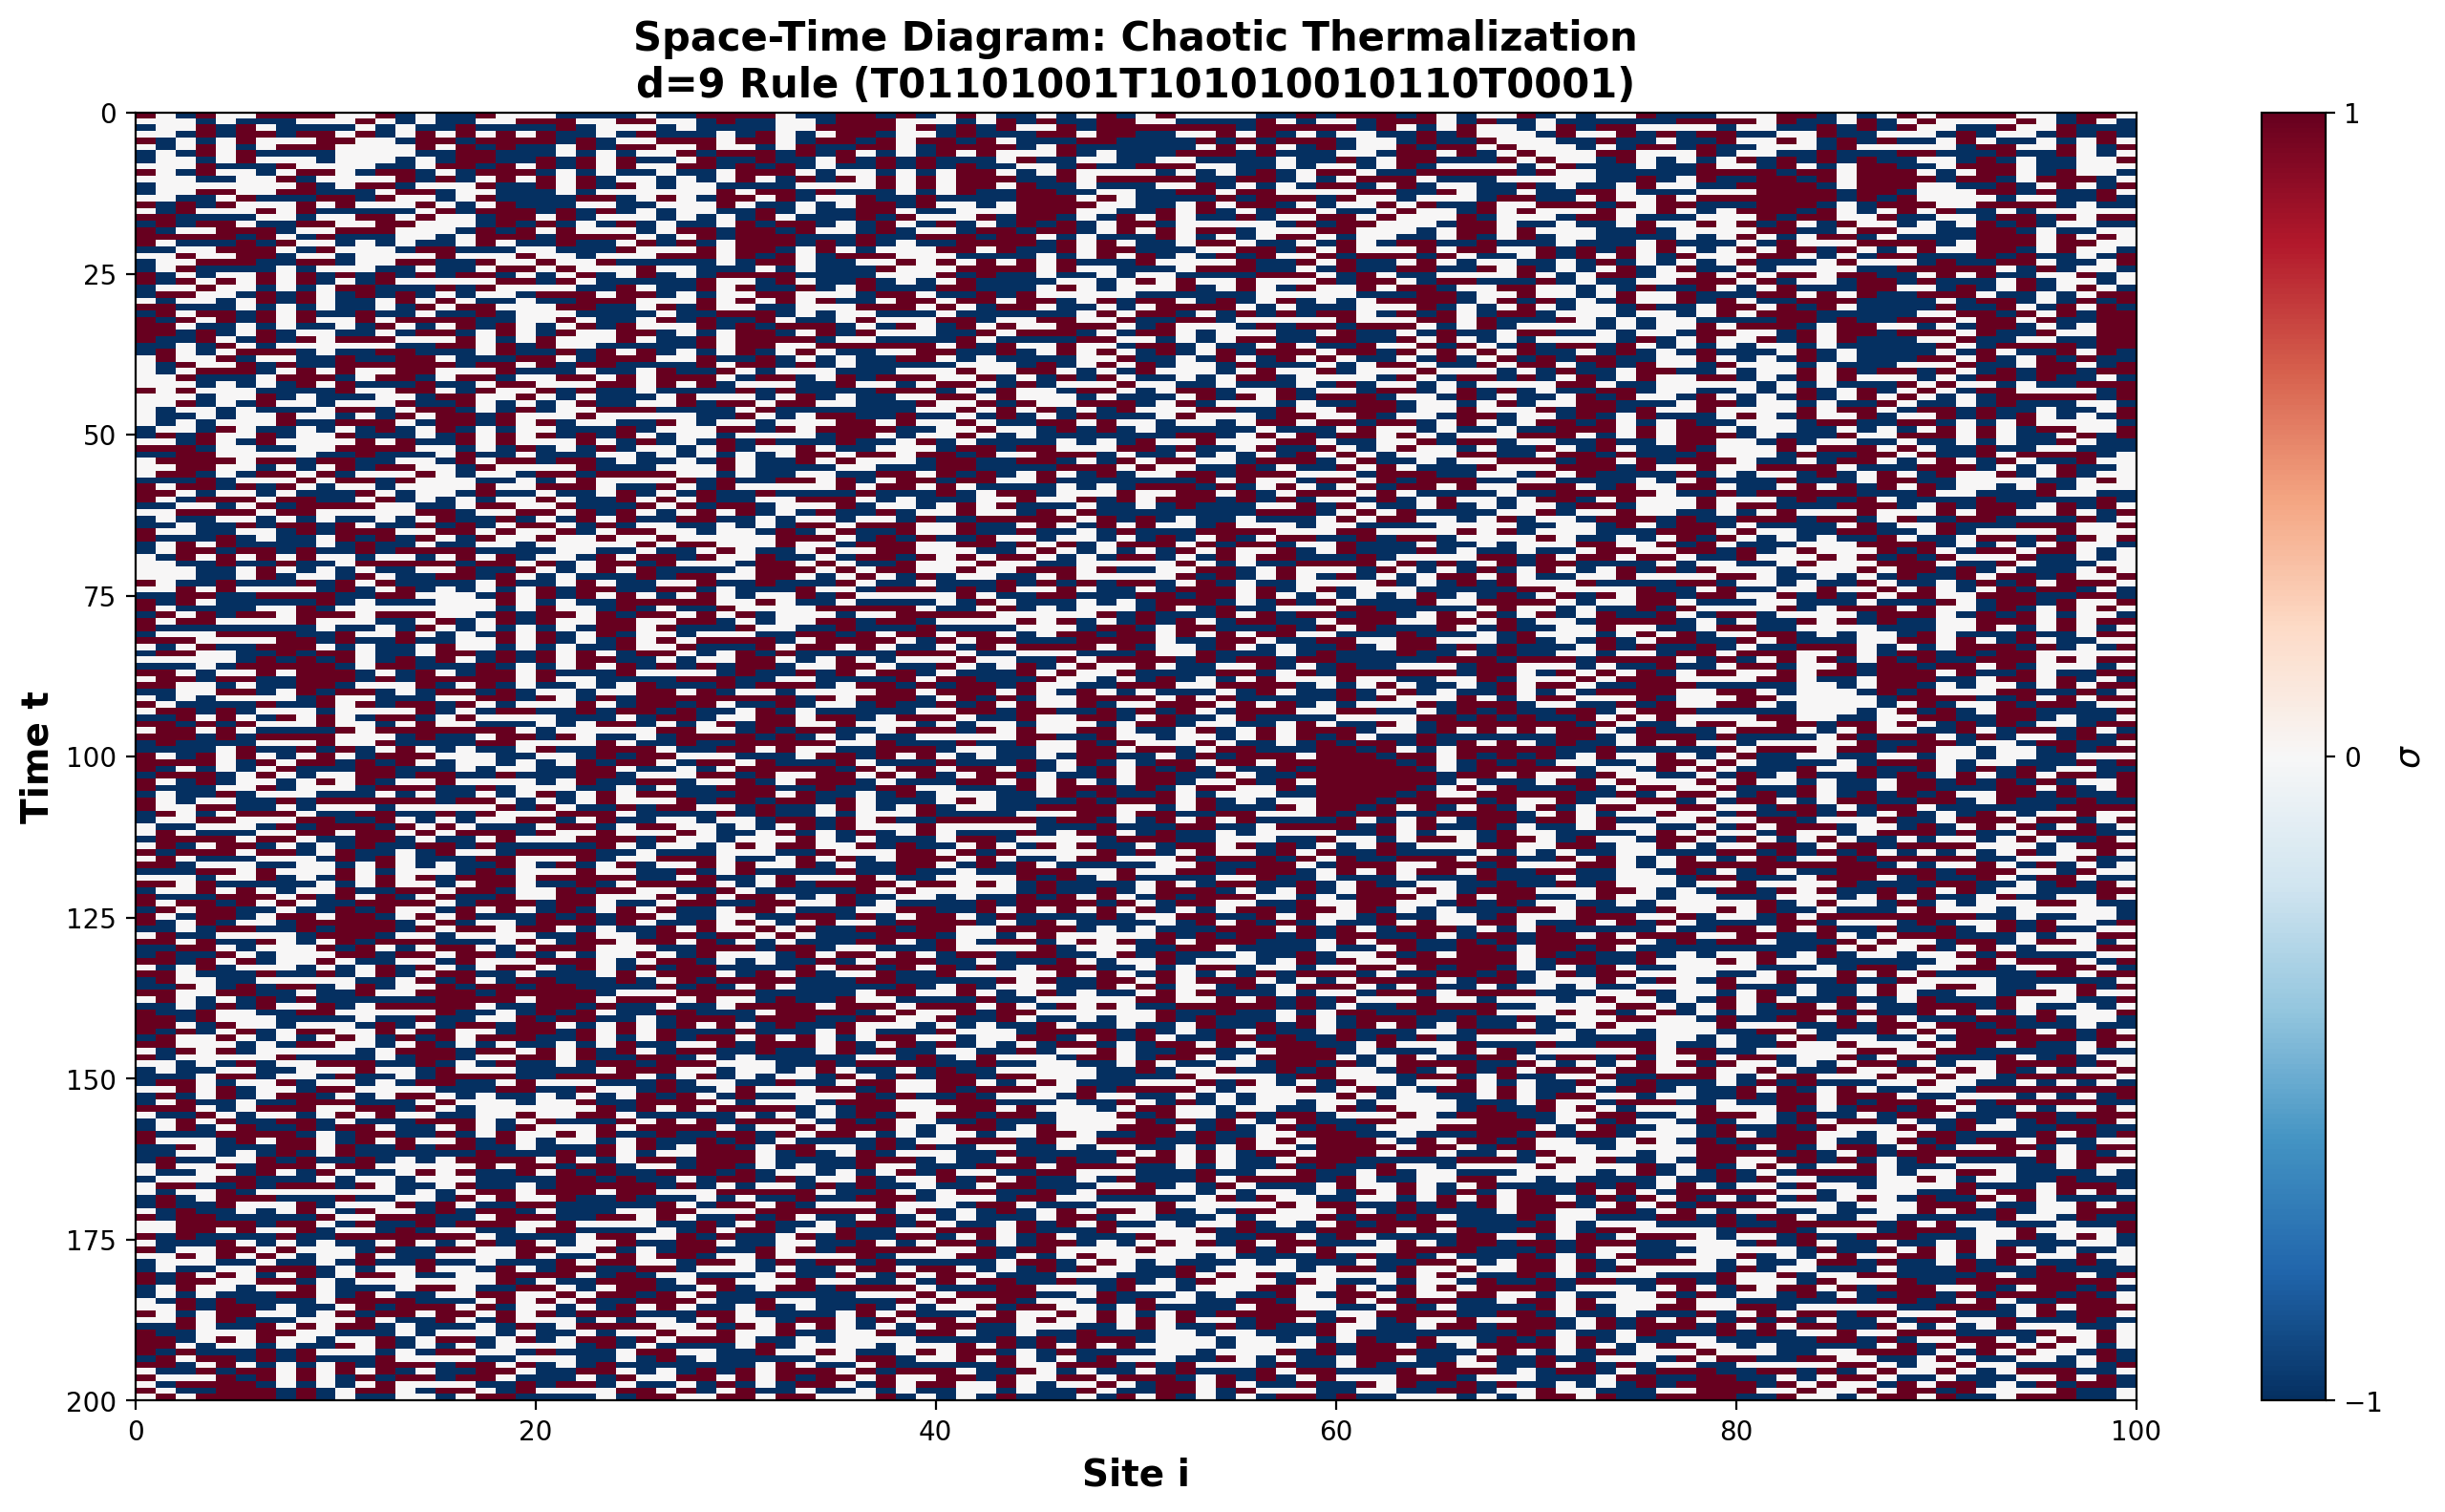
\includegraphics[width=0.45\textwidth]{image/spacetime_diagram_sigma.png} 
\caption{\label{fig:d9_spacetime}d=9的时空图表明系统没有出现非常强的周期性，系统发生明显混沌。}
\end{figure}

\begin{figure}[H]
\centering
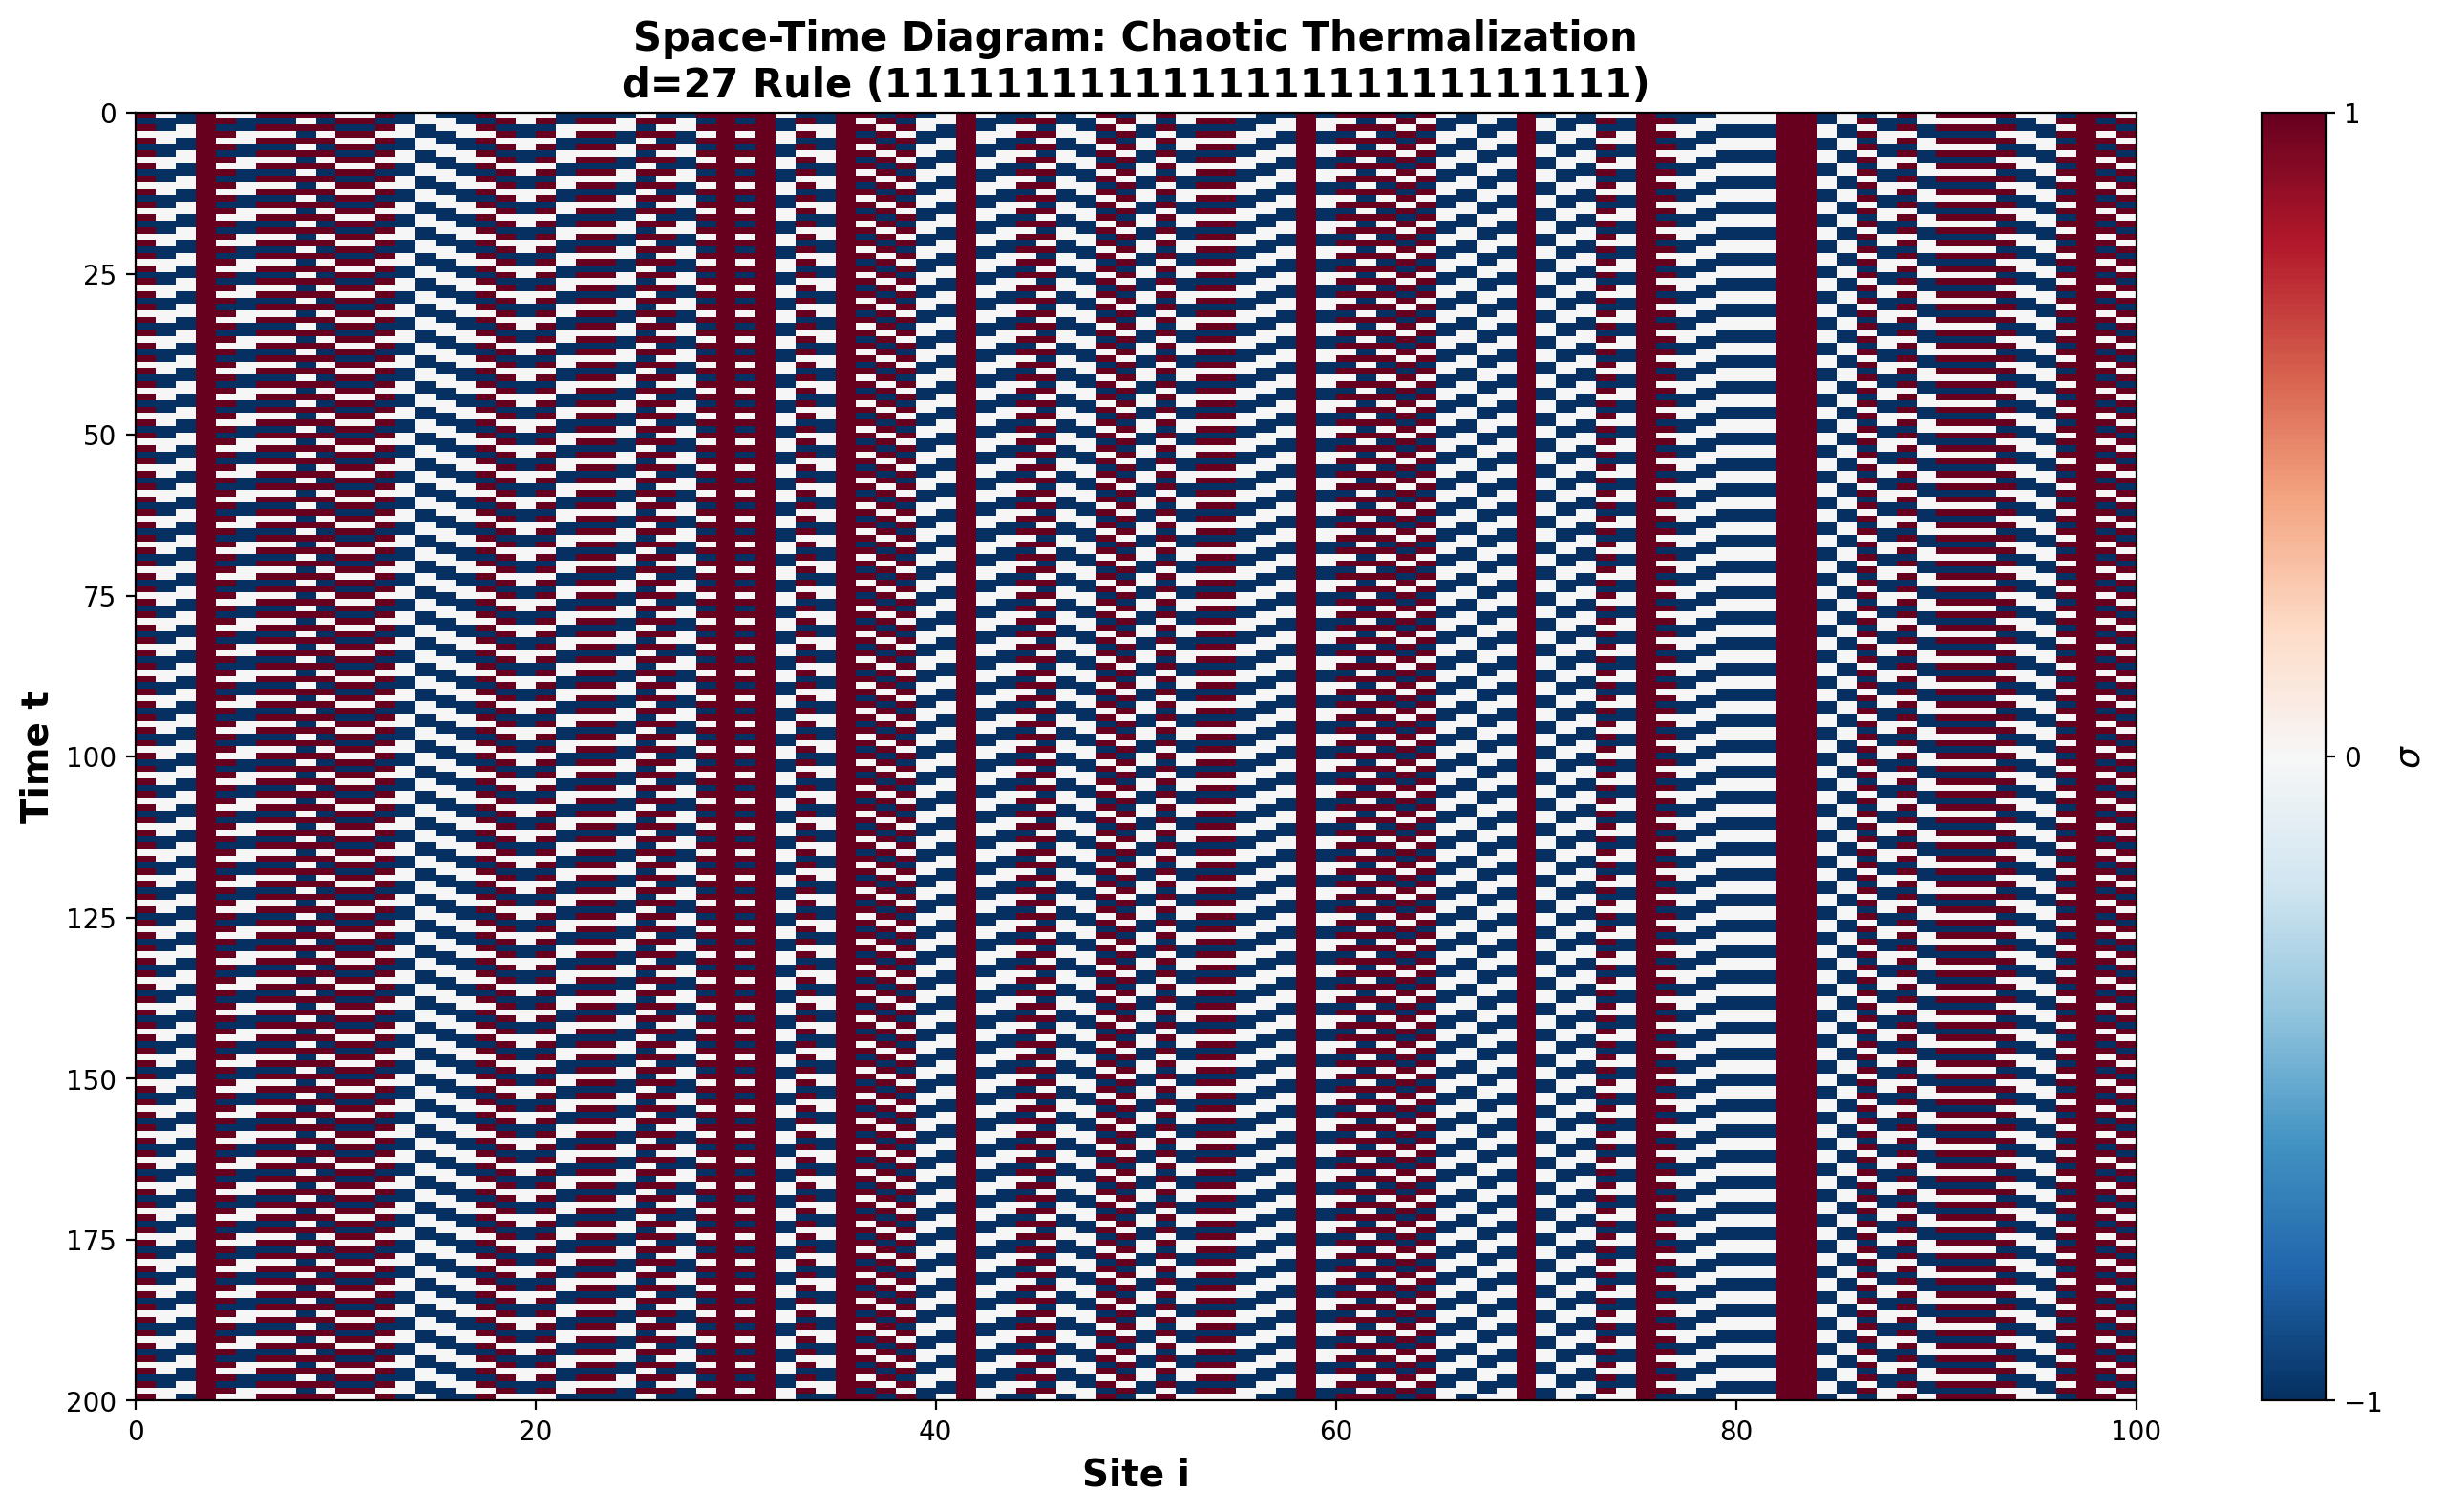
\includegraphics[width=0.45\textwidth]{image/spacetime_diagram_sigma_new.png} 
\caption{\label{fig:d27_spacetime}在d=27时空图中，体系以$T=4$进行演化，产生出非常强的局域性。}
\end{figure}

\subsubsection{轨道长度}
轨道结构是区分热化与非热化的最直接判据\cite{Yakov}。热化系统产生少量指数增长的长轨道，遍历相空间；
而非热化系统产生大量短周期轨道，被约束在守恒量定义的子流形上。轨道长度在热化类和非热化类之间存在系统性差异，
且这一差异随系统尺寸增大而扩大。轨道结构分析为 $d=9$ 作为热化判据提供了最强有力的动力学证据。

\begin{figure}[H]
\centering
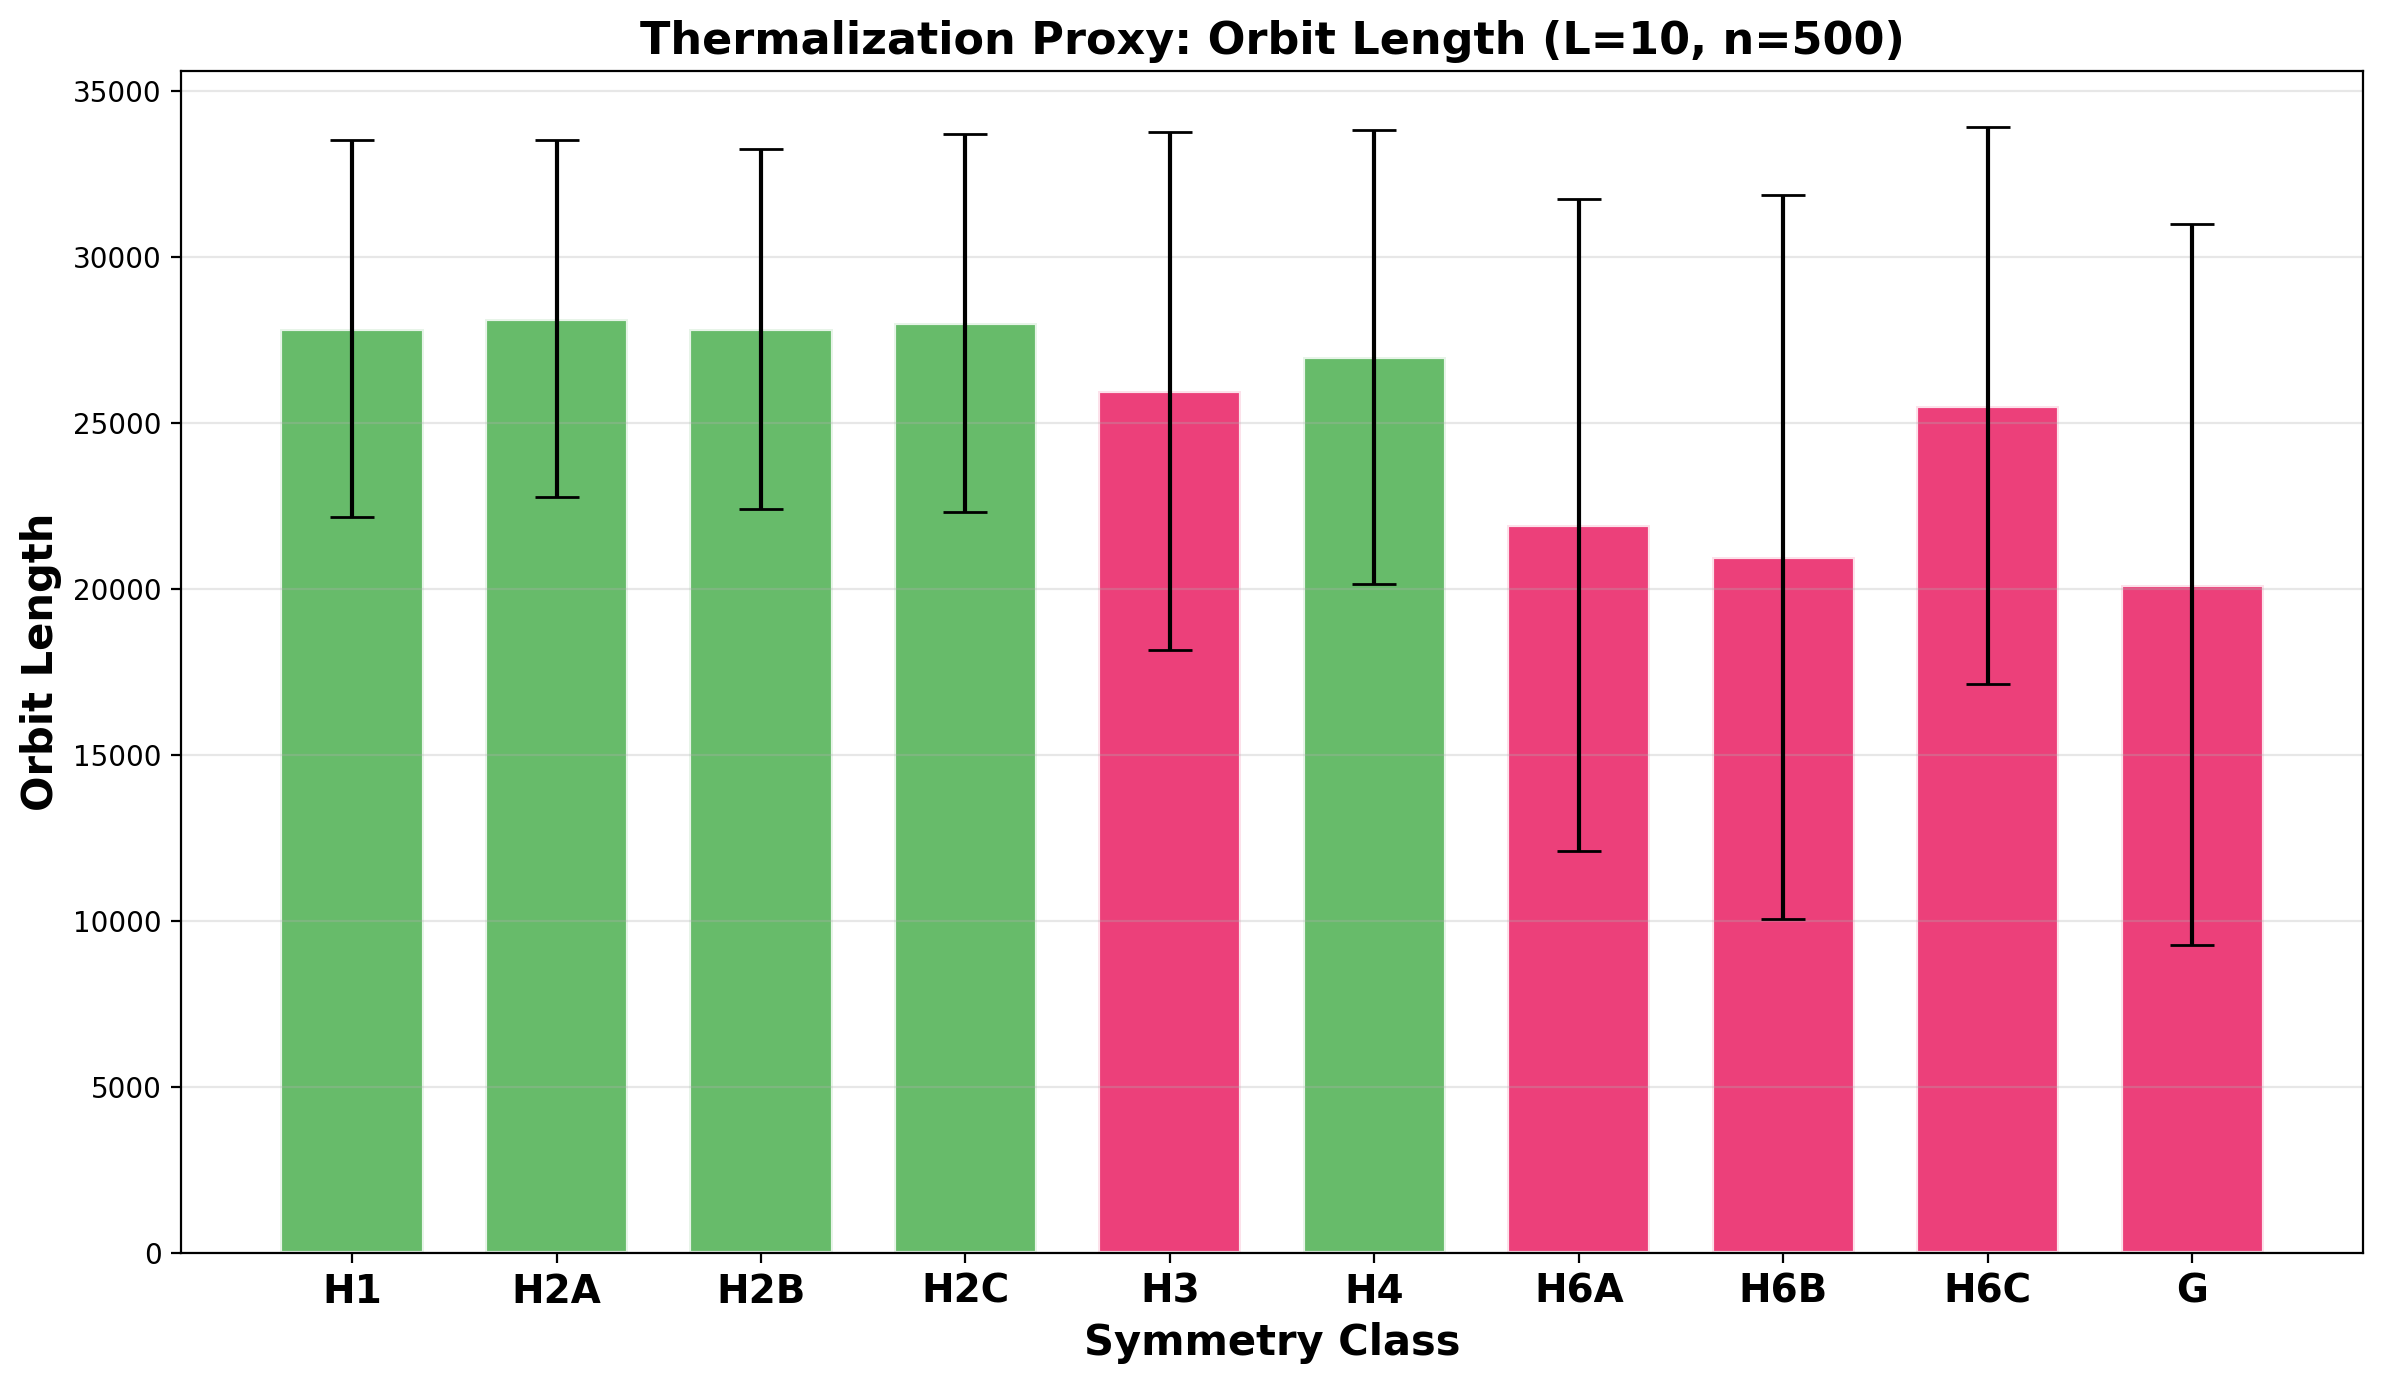
\includegraphics[width=0.45\textwidth]{image/fig3_orbit_length.png} 
\caption{\label{fig:d_orbit} 各对称类的轨道长度。热化类（绿色）的轨道明显长于非热化类（红色）。}
\end{figure}

图\ref{fig:d_orbit}展示了各对称类的轨道长度。
热化类（$\sim 28000$）的轨道明显长于非热化类（$\sim 20000-26000$）。G全对称类的轨道最短（20130），
受守恒量约束最严重。H$_1$的轨道最长（27831），遍历性最强。

\begin{figure}[H]
\centering
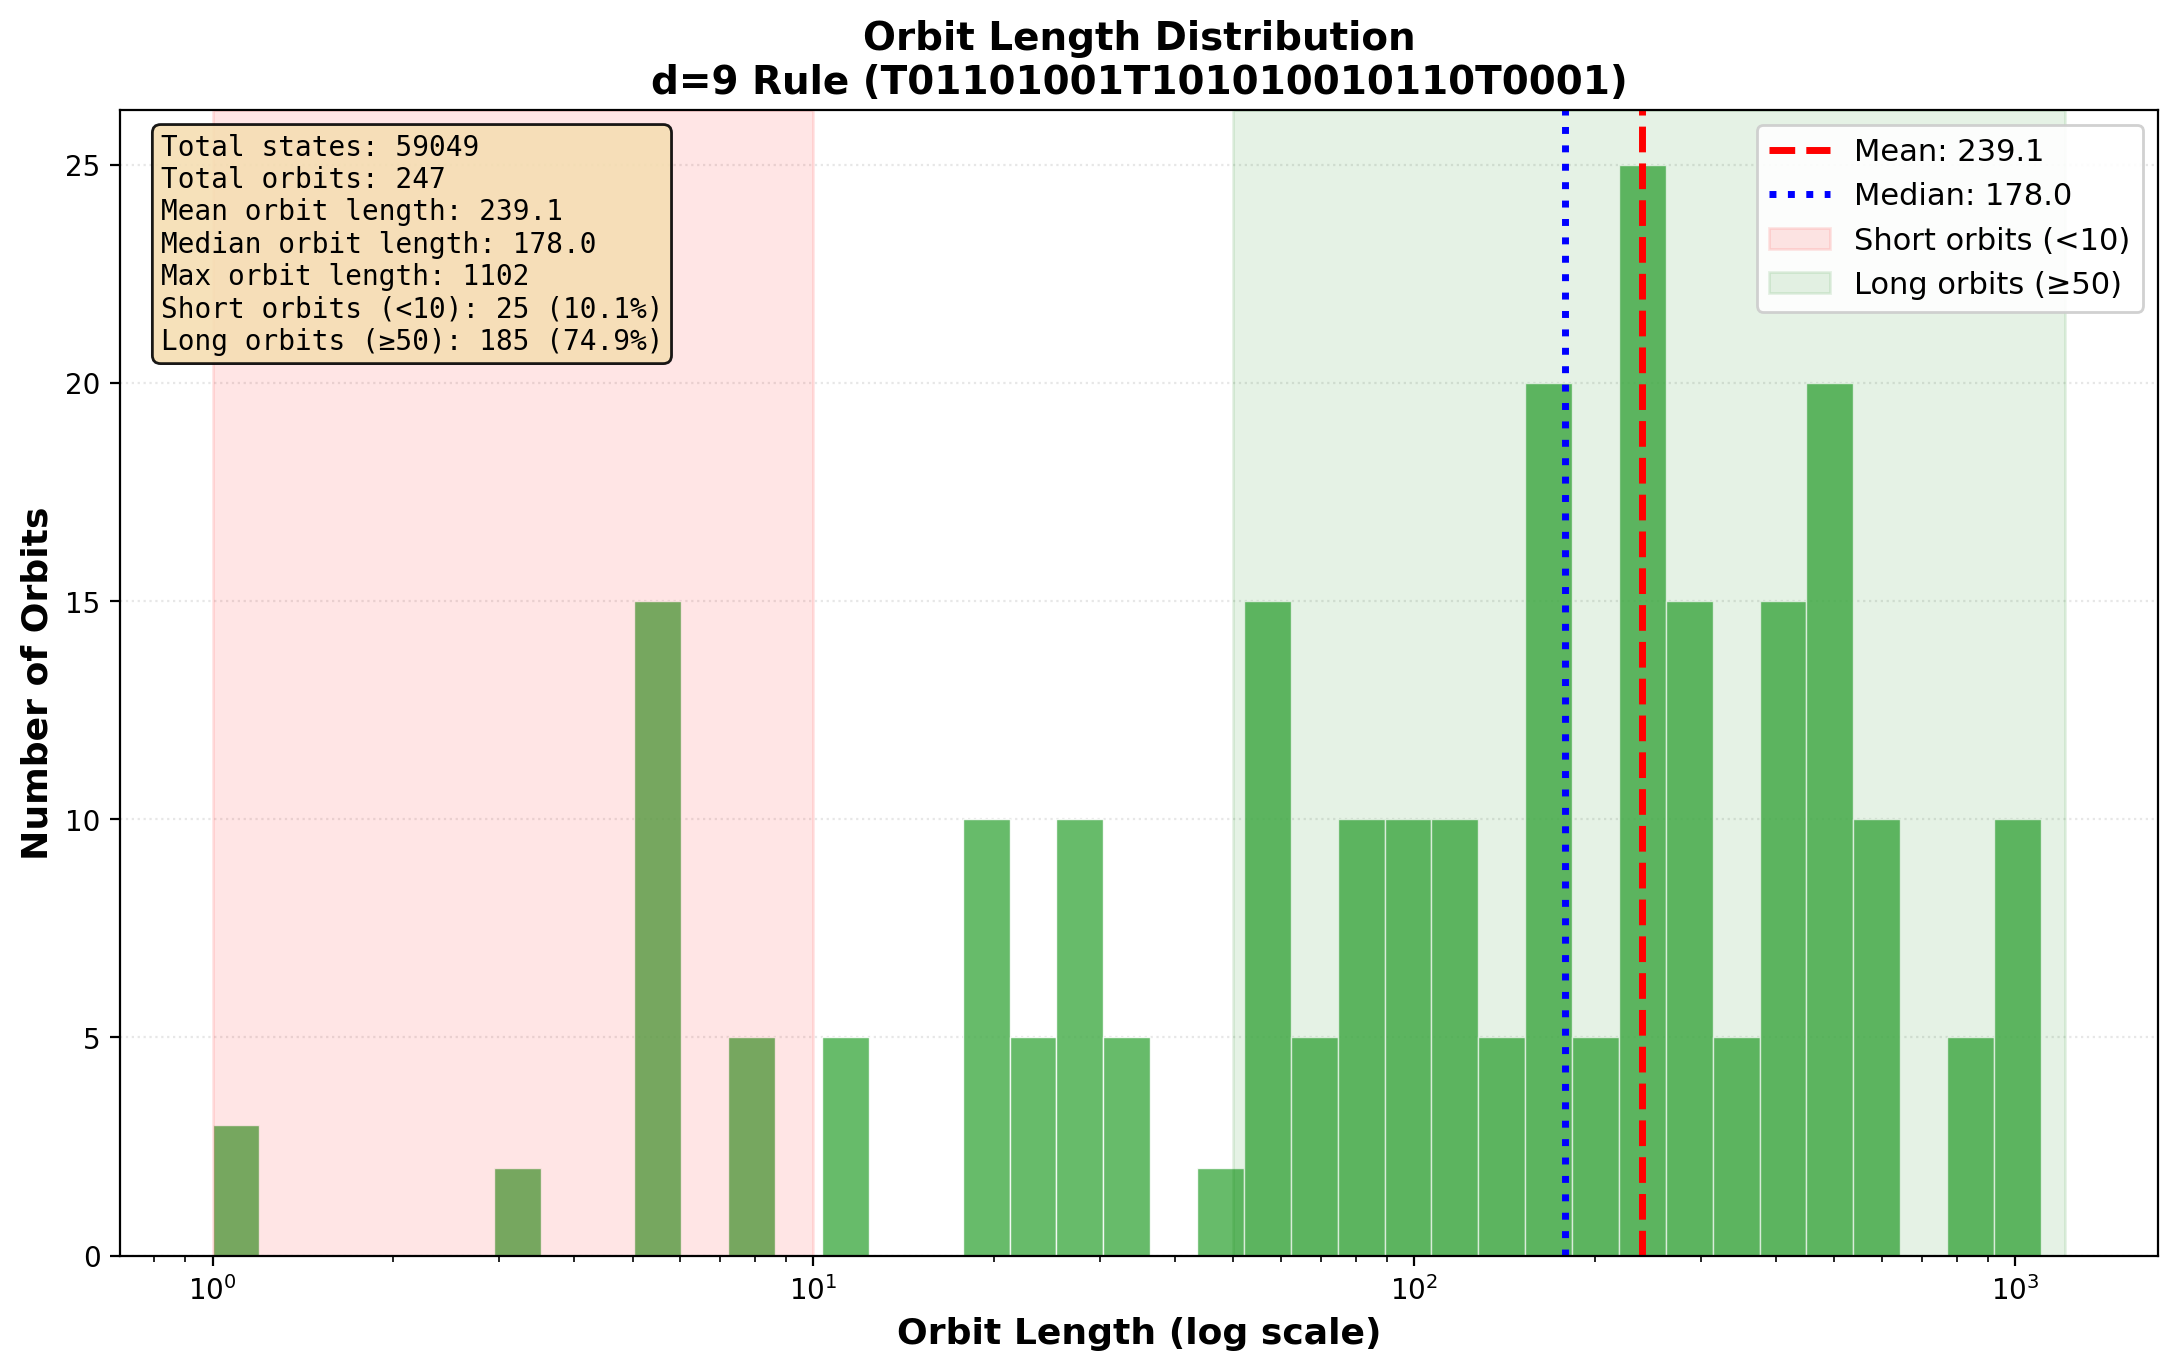
\includegraphics[width=0.45\textwidth]{image/3_orbit_structure.png} 
\caption{\label{fig:d9_orbit} 单条轨道覆盖相空间的显著部分，系统能够遍历大部分相空间。 }
\end{figure}

\begin{figure}[H]
\centering
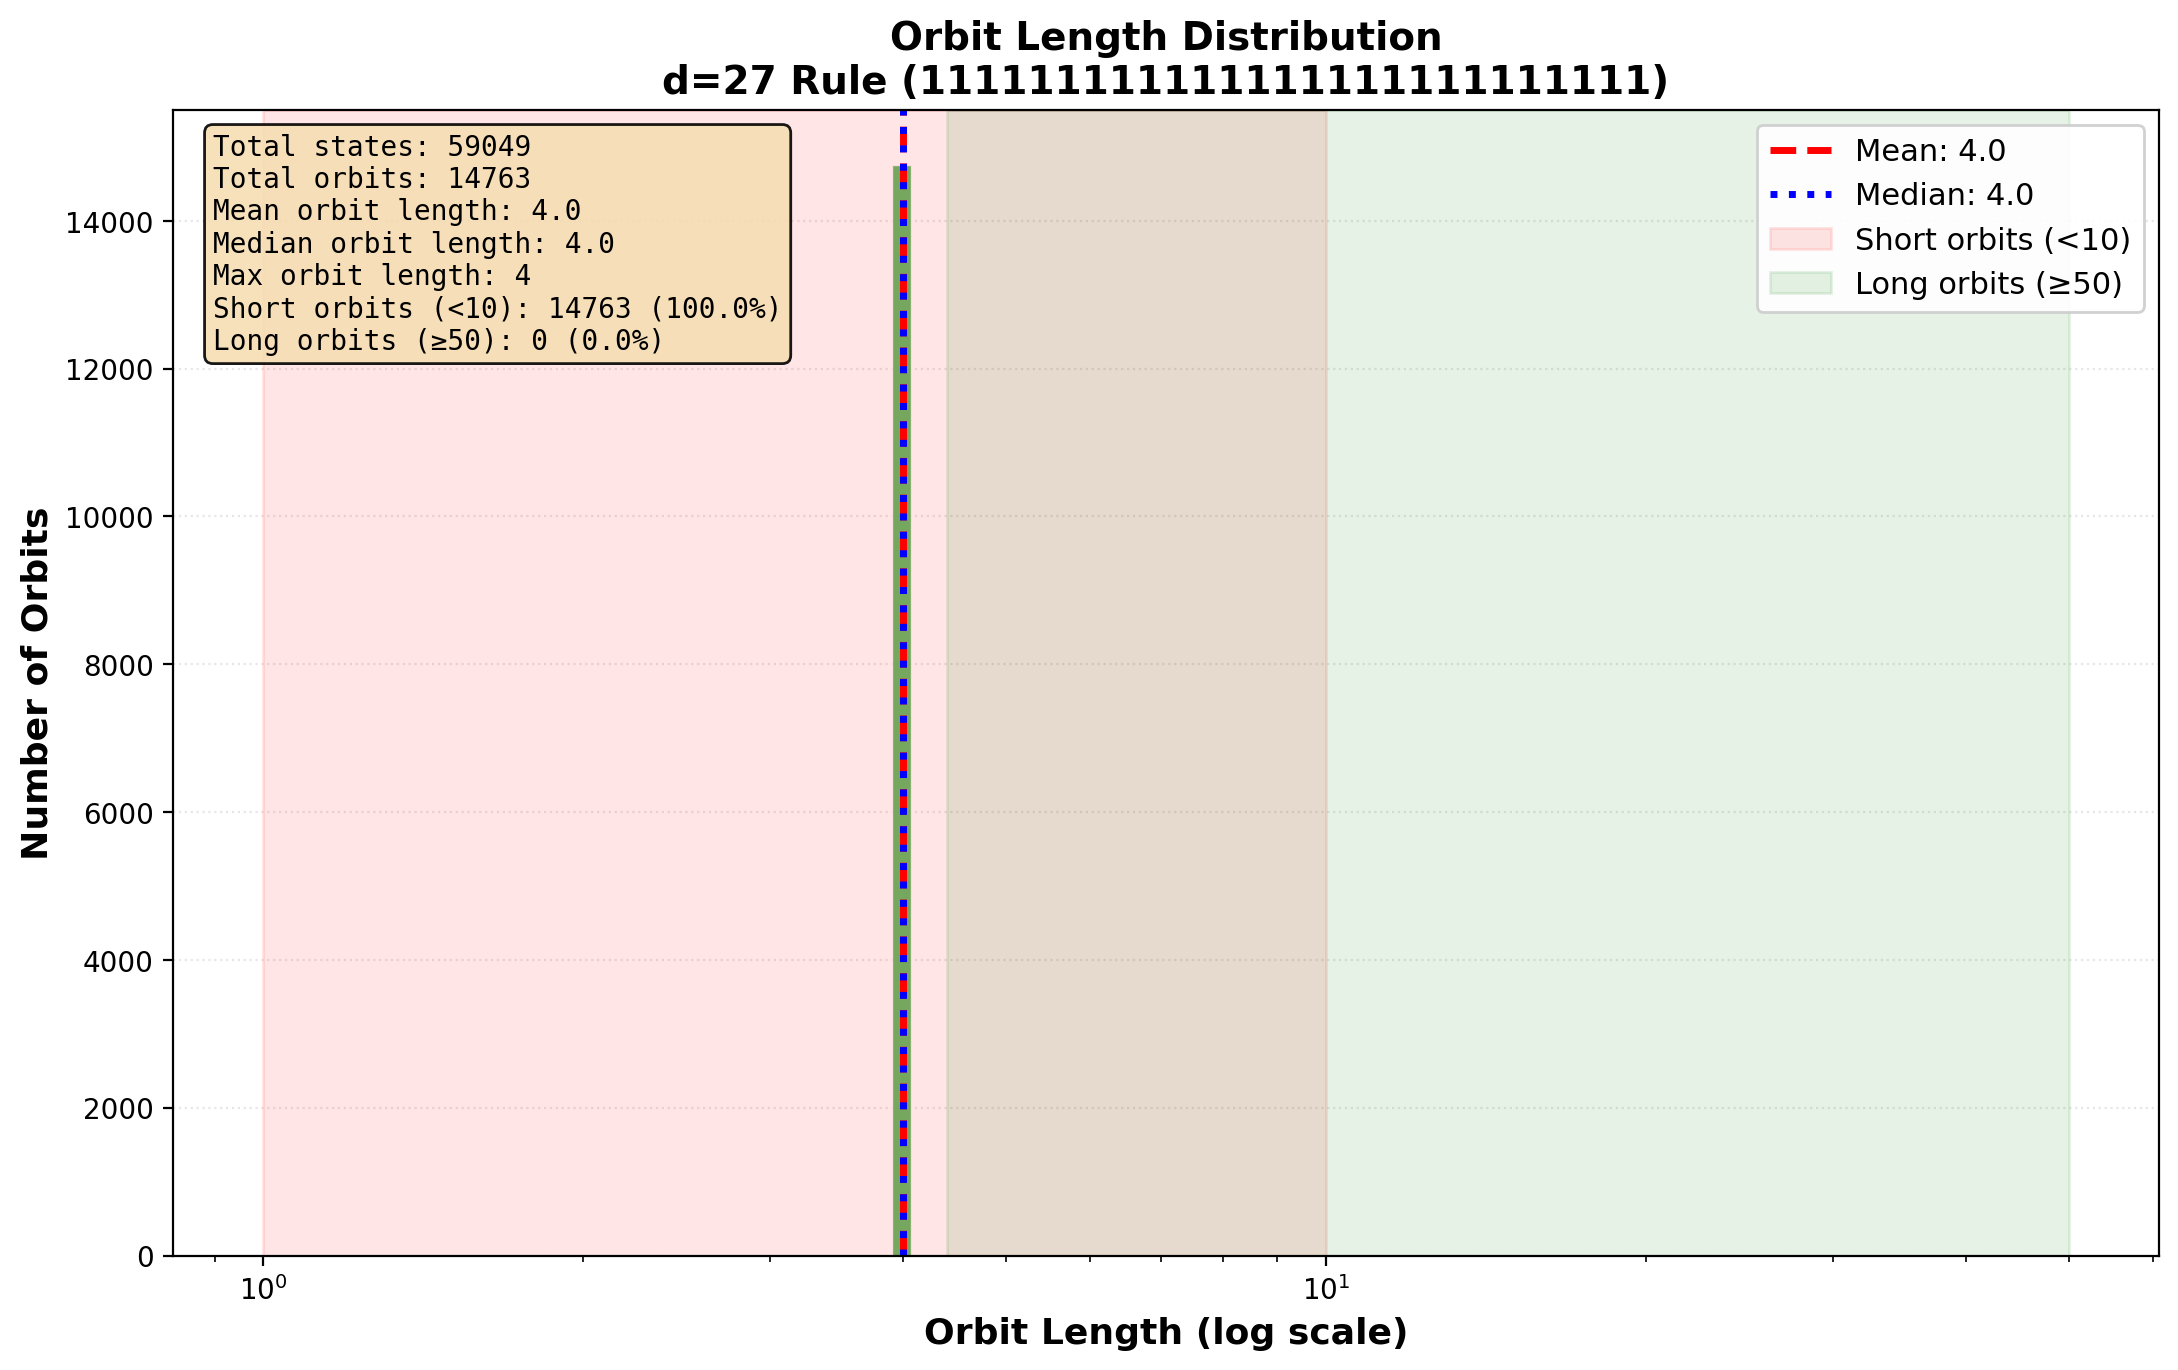
\includegraphics[width=0.45\textwidth]{image/3_orbit_structure_new.png} 
\caption{\label{fig:d27_orbit} 所有轨道长度严格为 4（或1），系统被束缚在极小区域内。}
\end{figure}

在$L=4$时（状态空间6561），该规则有127条轨道，平均长度$\langle T \rangle = 51.7$，最大轨道$T_{\max} = 348$。轨道长度随$L$指数增长：
$L=3$时$\langle T \rangle = 25.1$，$L=5$时$\langle T \rangle = 239.1$，$L=8$时采样均值达9375。
作为对比，d=27的常值规则（$f \equiv 1$）在$L=4$时有1641条轨道，全部长度严格为4，轨道数随$L$以$9^L/4$增长。这种超短的轨道无法使系统热化。

我们进一步猜测，轨道长度出现的概率随着长度的变化关系存在幂律：
\begin{equation}
    P(T) \varpropto T^{-\alpha}
\end{equation}
但经过采样模拟后，我们发现$\alpha$并不是一个普适性的常数，$\alpha$依赖于$f$的选取即系统的微观细节。

\subsubsection{Lyapunov指数}
对于两个不同对两个长度均为$2L$的构型$c_1,c_2$和（每个格点有$r$和$\sigma$两个自由度），定义 $Hamming$ 距离：
\begin{equation}
    D(t) = \sum_{i=0}^{2L-1} 1[c_{1,i}(t) \neq c_{1,i+1}(t)]
\end{equation}
这个量统计了两个构型在多少个格点自由度上取值不同。
在扰动远未饱和的早期阶段$(0 < D(t) < 2L\times 0.8)$假设有指数增长：
\begin{equation}
    D(t) \sim D(0) e^{\lambda t}
\end{equation}
其中，$\lambda$ 被称为 Lyapunov指数\cite{Ljapunov}。我们期望热化系统中局部扰动会迅速扩散到全局，Hamming 距离快速增长；非热化系统扰动被局域，Hamming 距离不增长。
若体系$\lambda > 0 $， 则系统对初始扰动敏感，呈混沌特征。

\begin{figure}[H]
\centering
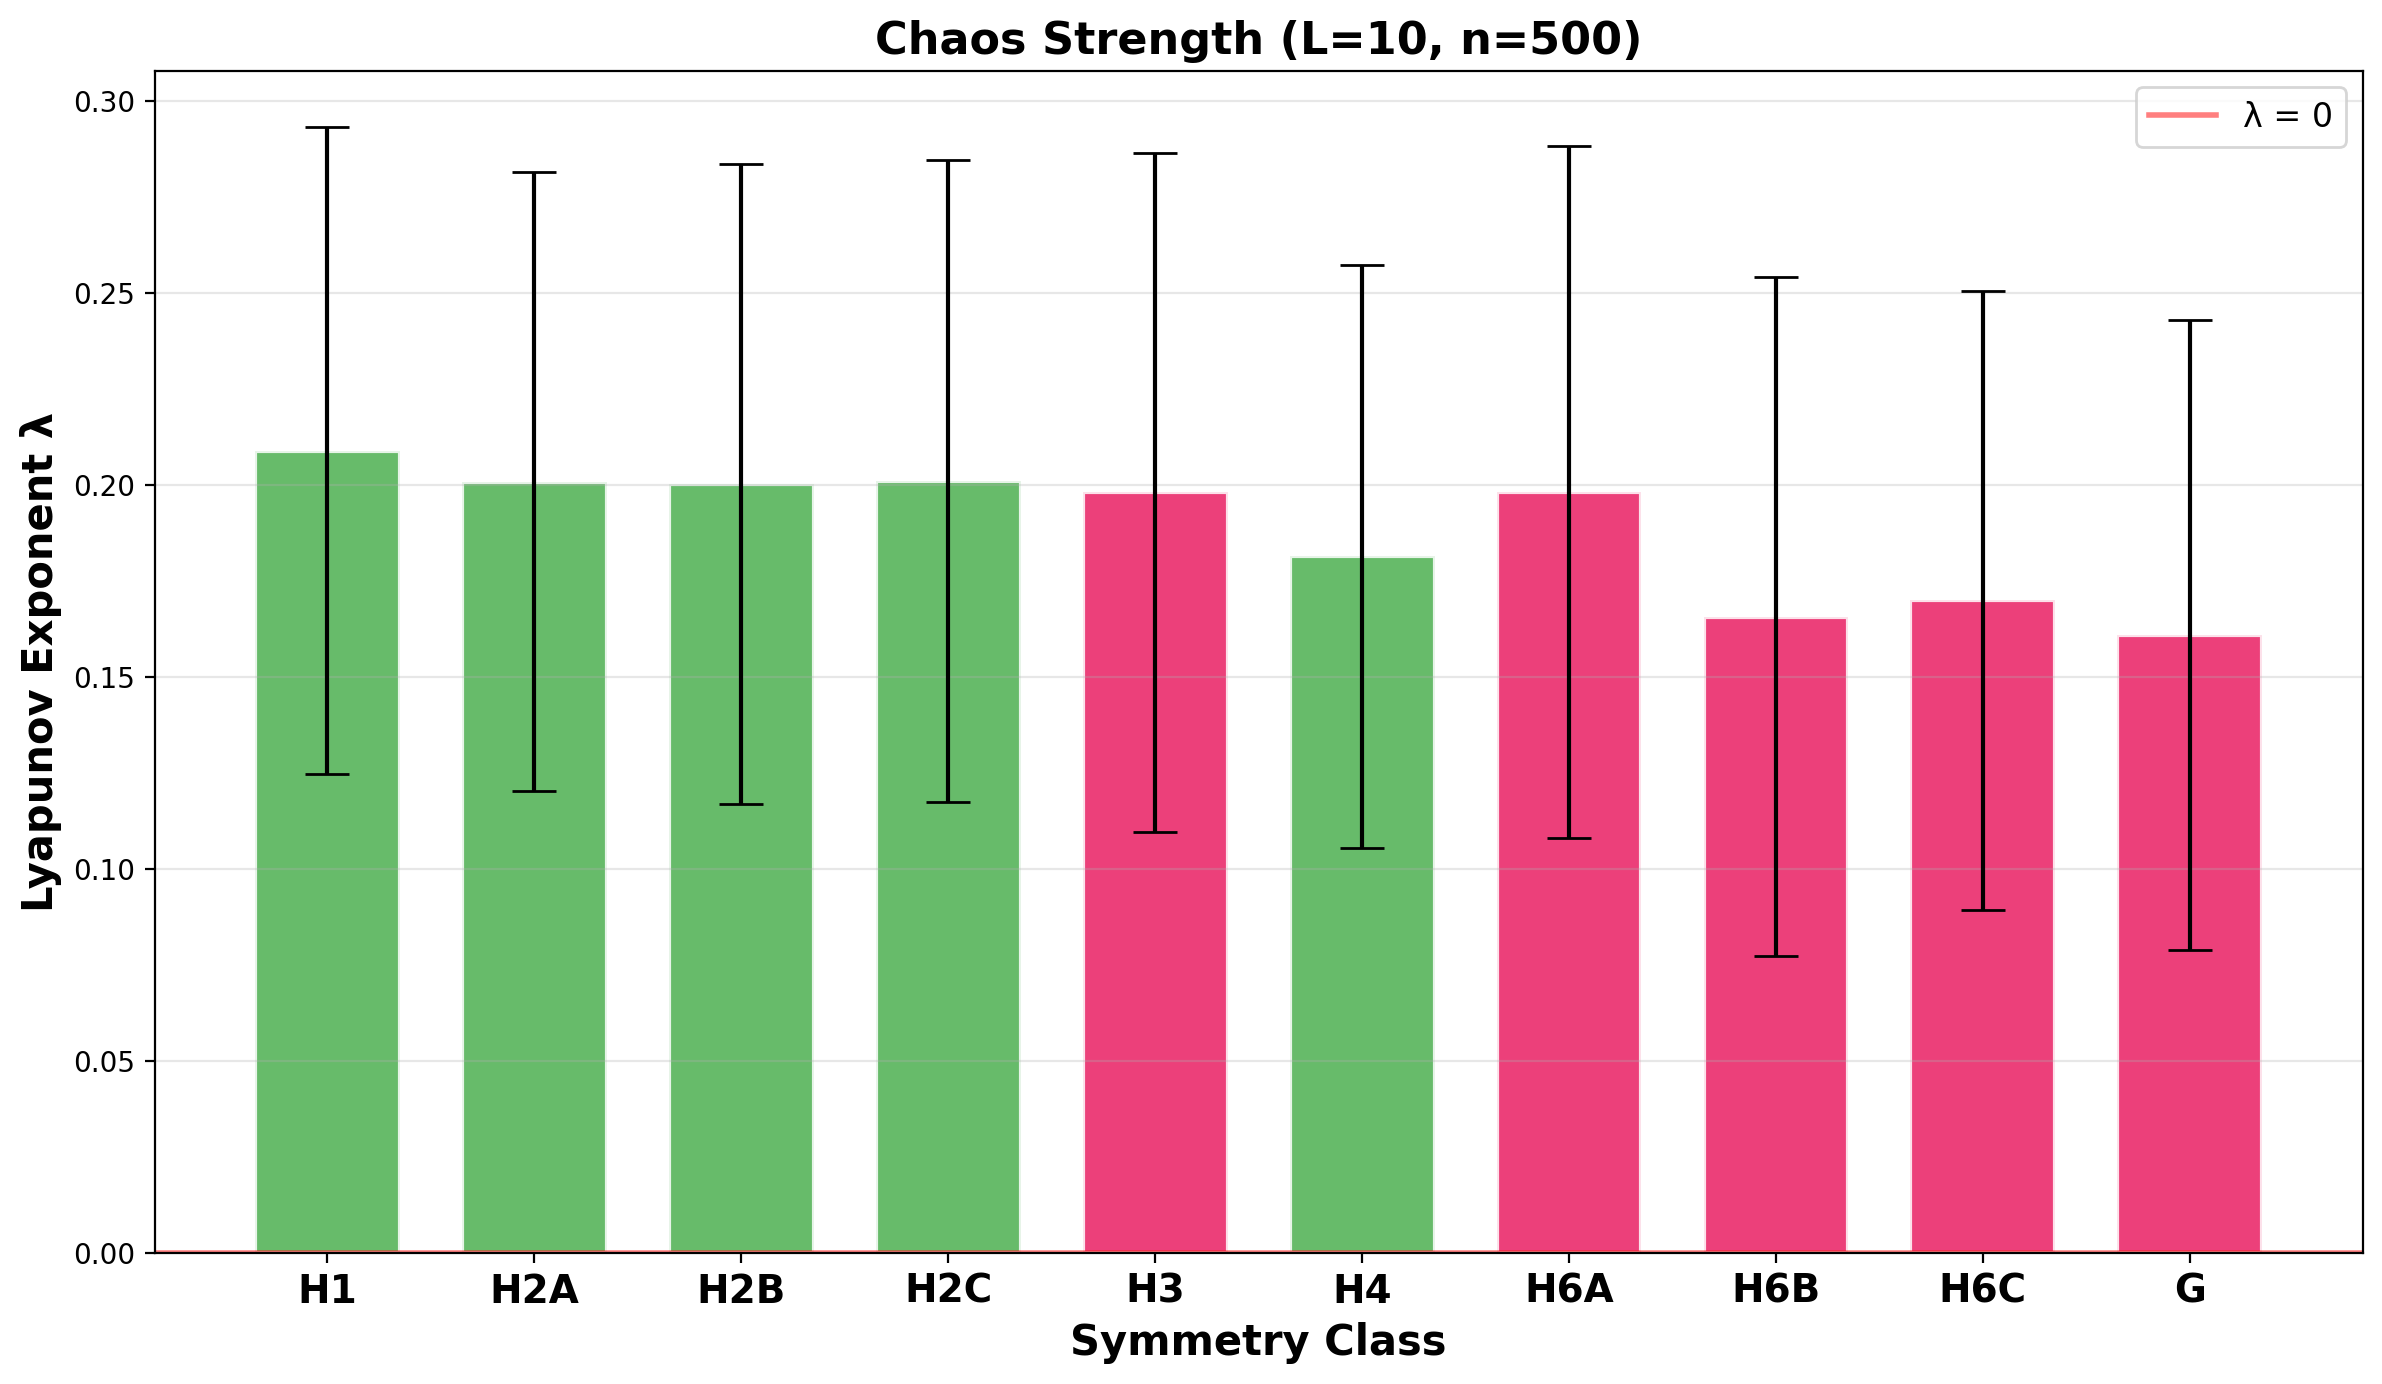
\includegraphics[width=0.45\textwidth]{image/fig2_lyapunov.png} 
\caption{\label{fig:d_lyapunov} 各对称类的Lyapunov指数。所有类的$\lambda > 0$。绿色柱为热化类，红色柱为非热化类。}
\end{figure}

虽然非热化类的$\lambda$系统性地低于热化类（约低15-20\%），但是我们期望在满足热力学极限$L \to \infty ， T \to \infty$下，所有$d>9$的规则都会导致体系的$\lambda$为0。而现在出现的这种错觉这可能是由于体系尺度太短或演化时间太短导致在拟合时候出现的误差。

\begin{figure}[H]
\centering
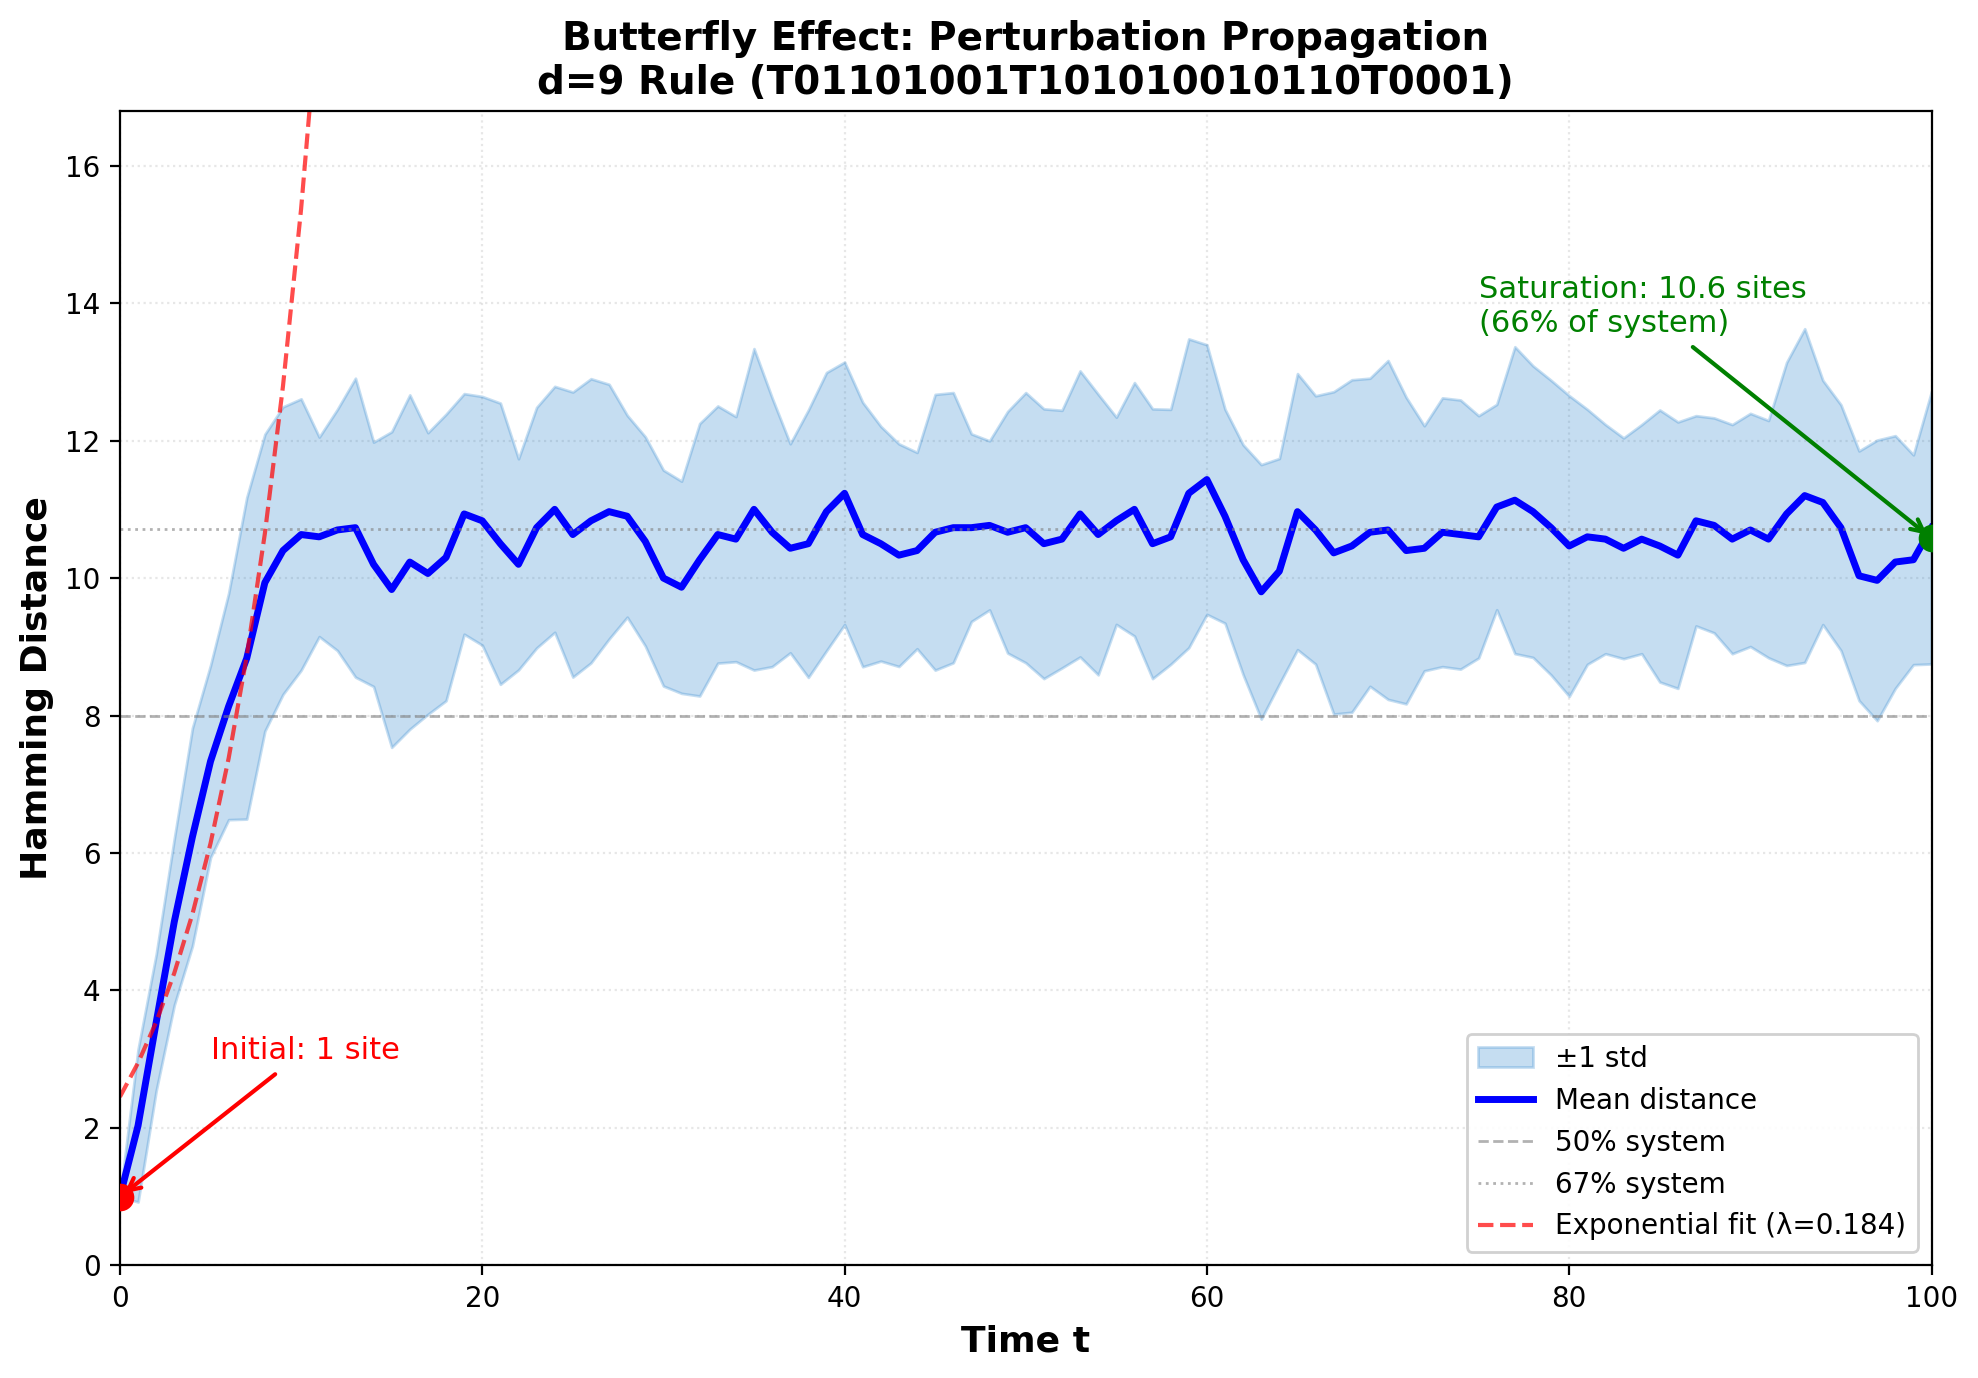
\includegraphics[width=0.45\textwidth]{image/1_butterfly_effect.png} 
\caption{\label{fig:d9_Lyapunov} 局部的扰动被迅速扩散到全局，$\lambda \approx 0.184$ 体系呈扩散特征。 }
\end{figure}

\begin{figure}[H]
\centering
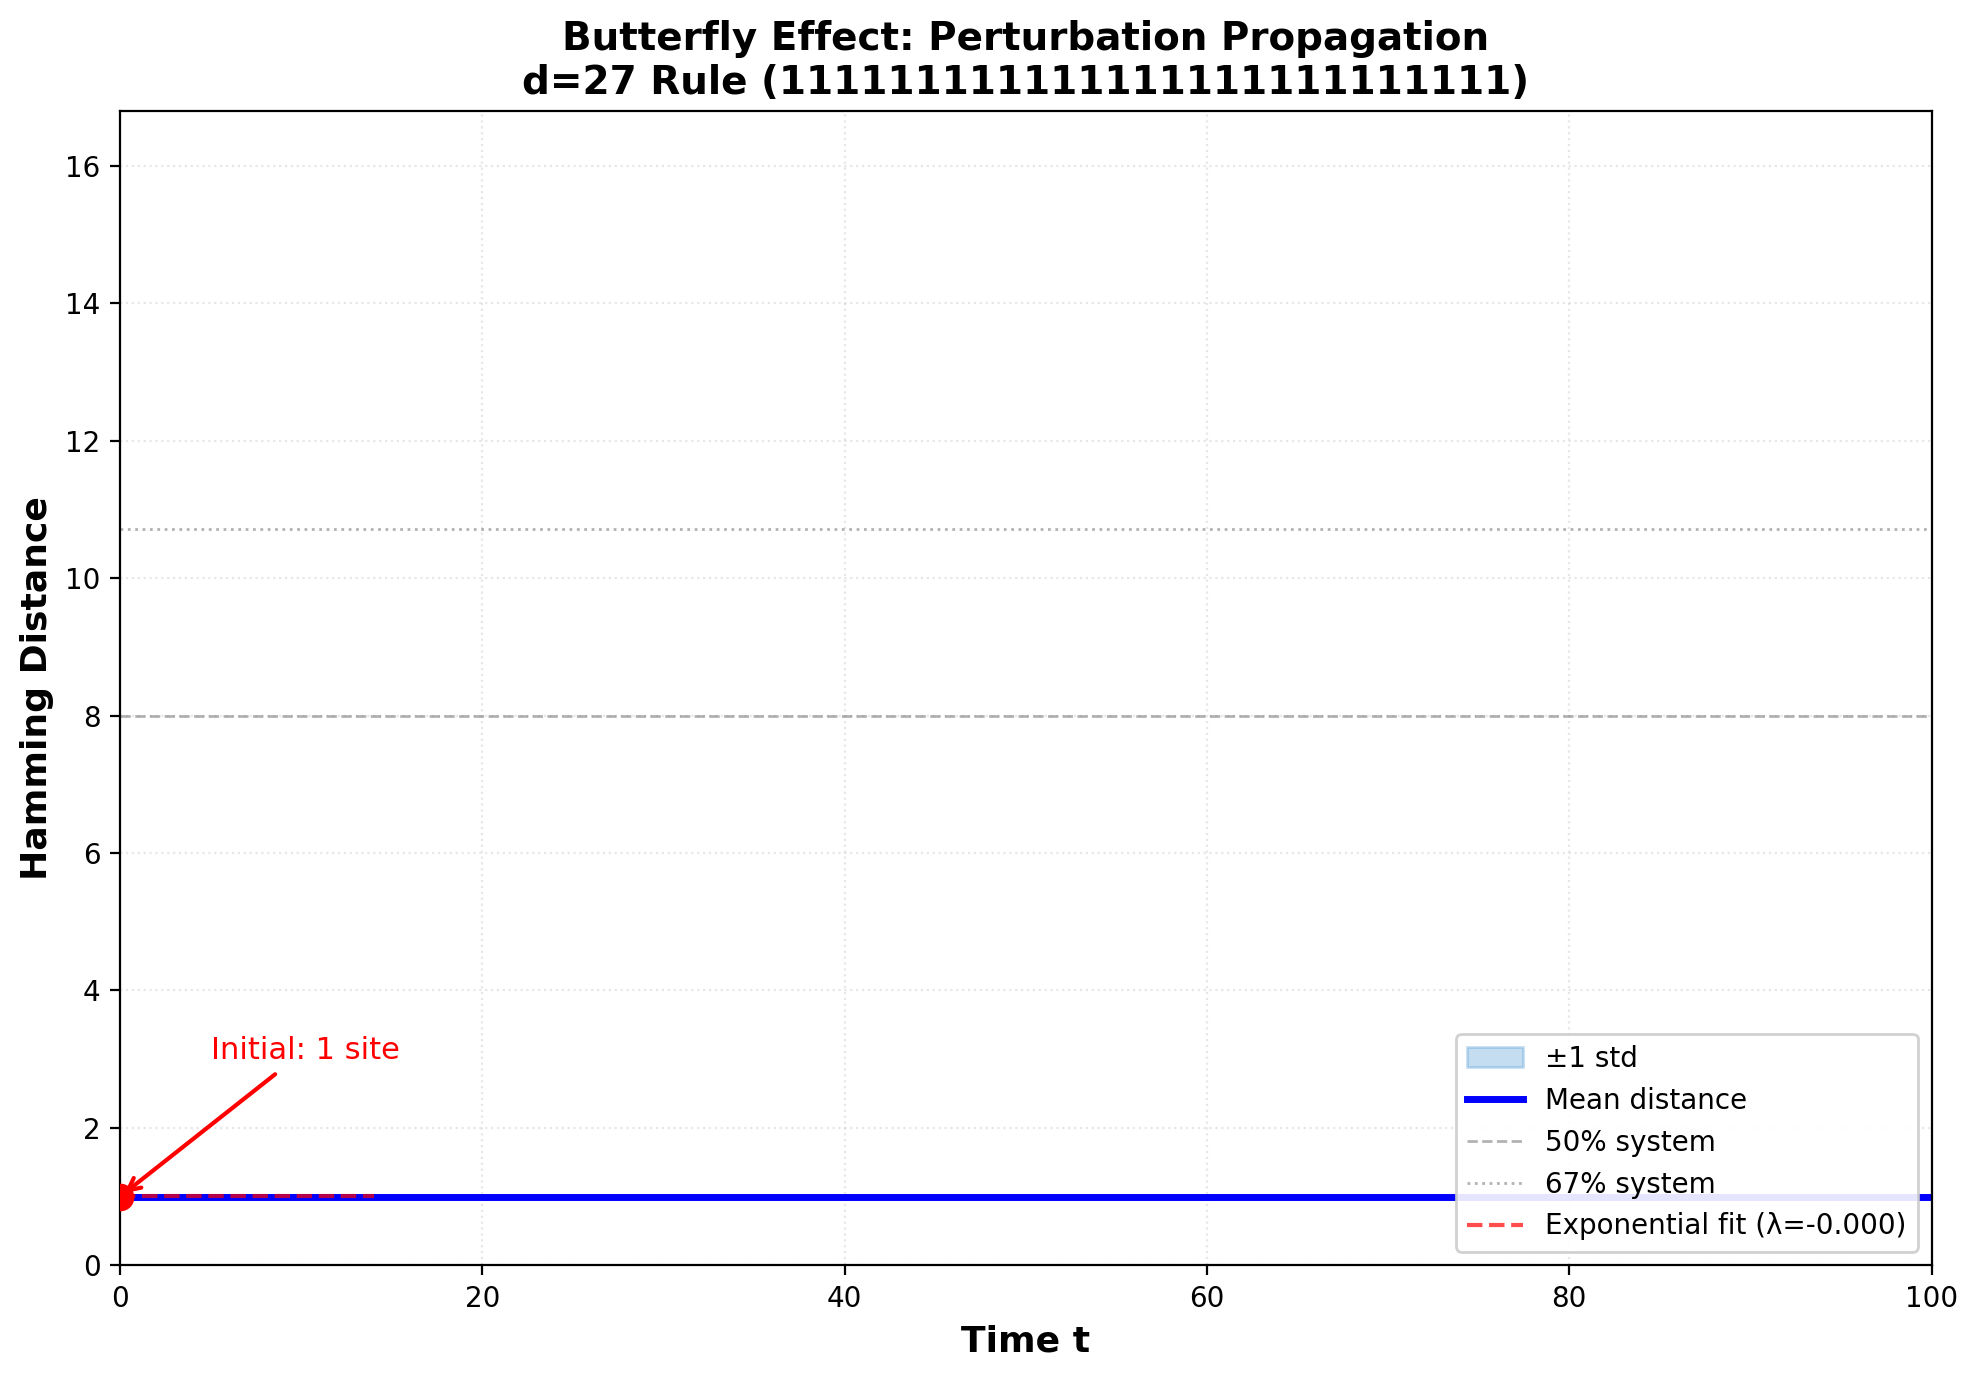
\includegraphics[width=0.45\textwidth]{image/1_butterfly_effect_new.png} 
\caption{\label{d27_Lyapunov} 扰动被局域化，体系不呈热化性质。}
\end{figure}

我们对500个随机$d=9$规则的Lyapunov指数进行统计（$L=6$）发现：100\%的规则$\lambda > 0$，分布符合Gaussian分布（KS检验$p=0.97$），均值$\bar{\lambda} = 0.045$，标准差$\sigma_\lambda = 0.006$，如图\ref{Lyapunov}所示：

\begin{figure}[H]
\centering
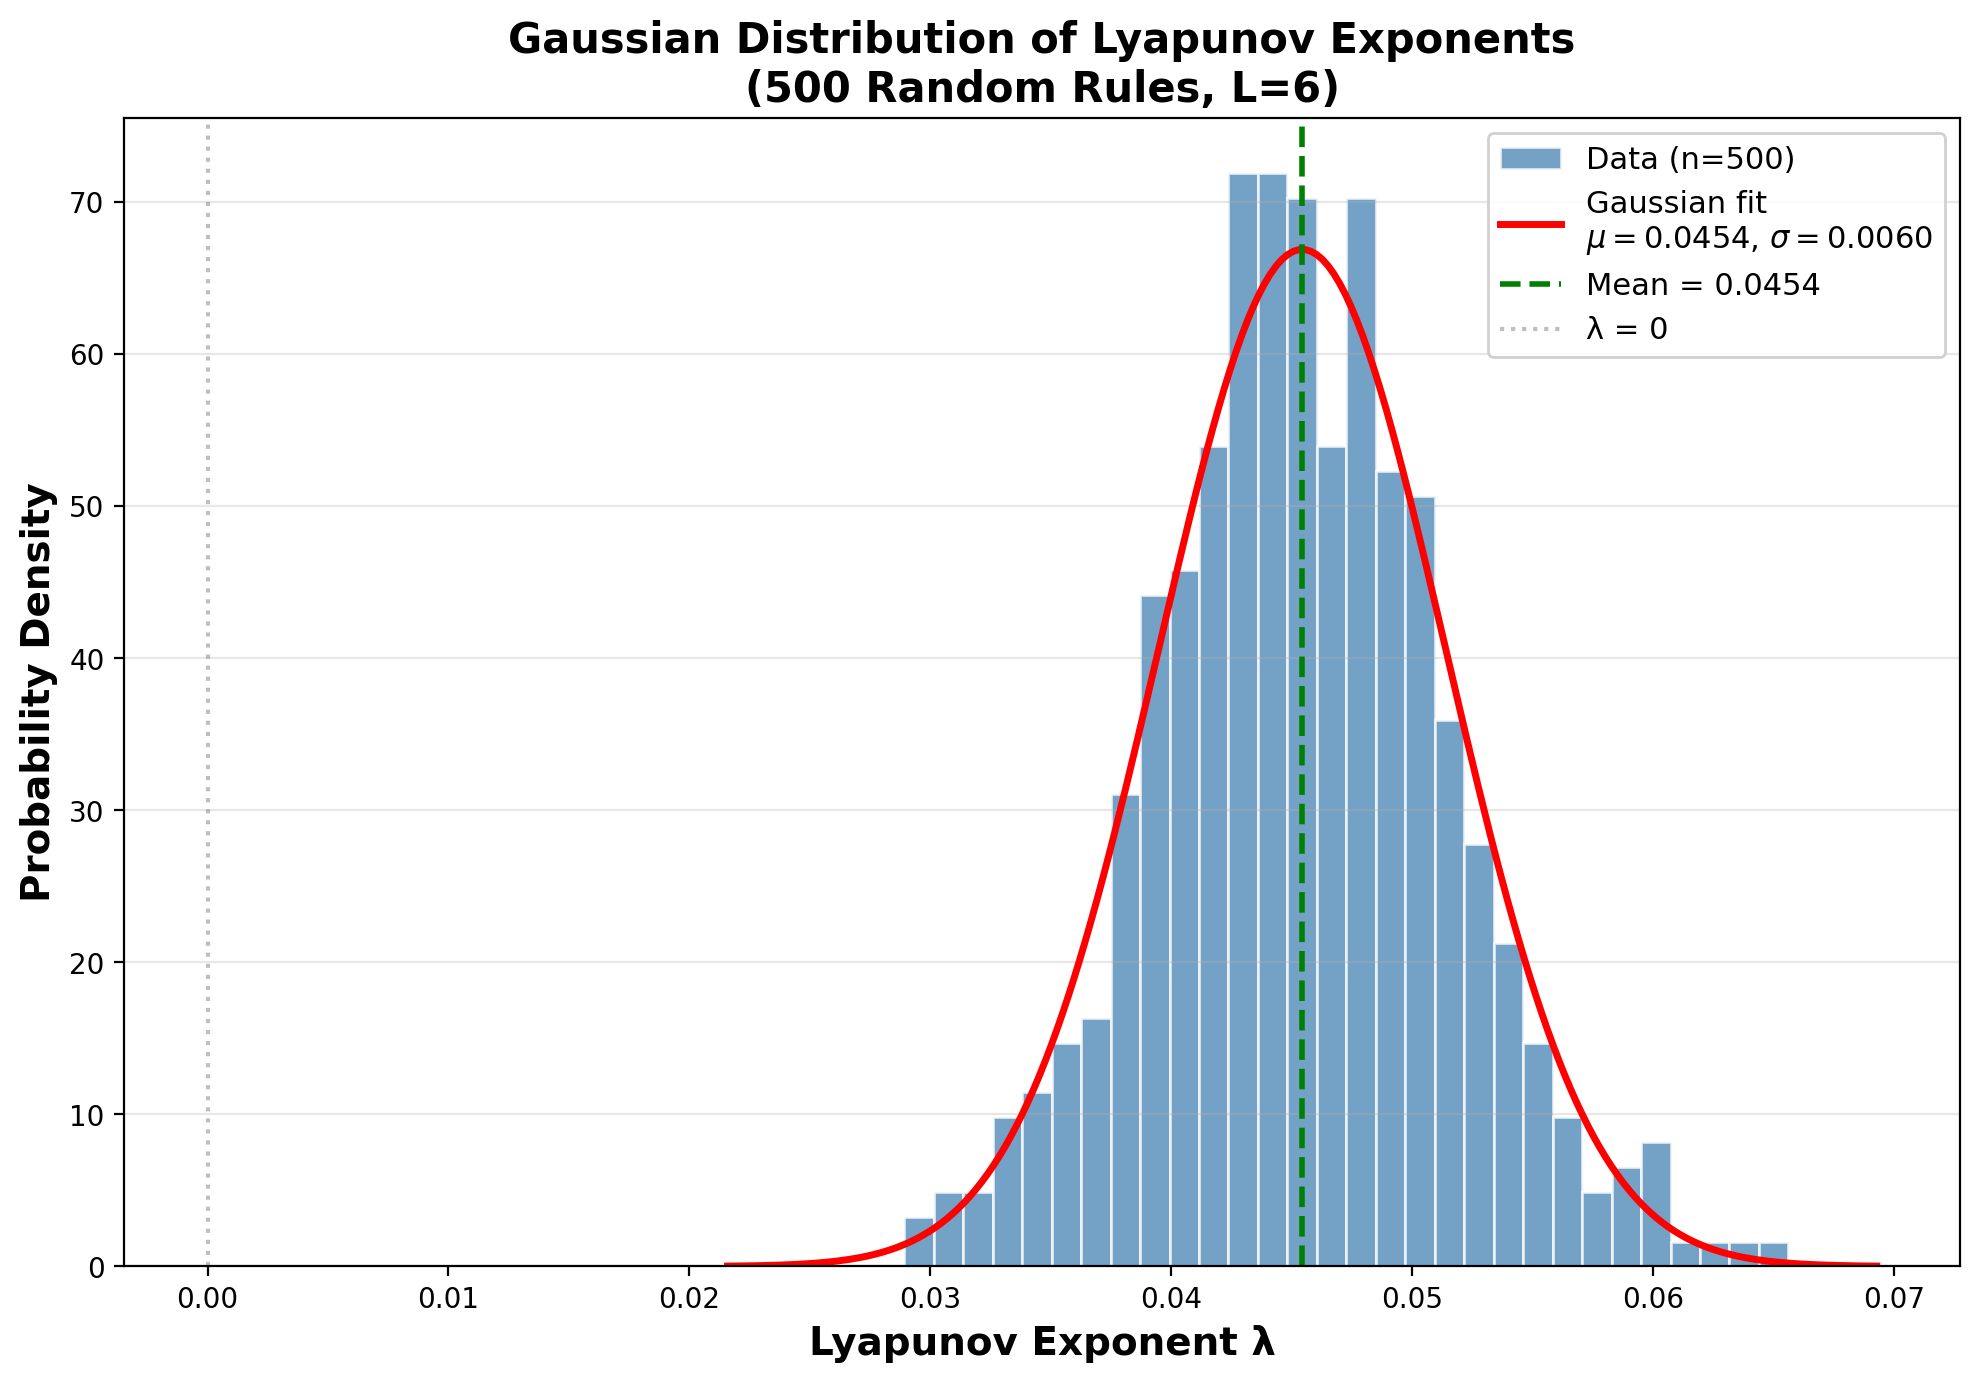
\includegraphics[width=0.45\textwidth]{image/lyapunov_gaussian.png} 
\caption{\label{Lyapunov}  $\lambda $ 满足高斯分布 。}
\end{figure}

在进一步的分析中，我们对20个固定规则在$L=4$至$L=100$下的Lyapunov指数进行有限尺寸标度分析。
数据拟合$\lambda(L) = \lambda_\infty + c/L^{\alpha}$，最佳拟合指数$\alpha \approx 0.5$，
热力学极限$\lambda_\infty \approx 0.060 > 0$。这确证了系统在$L \to \infty$时保持混沌。
这说明$\lambda$是强度量，不随系统大小变化，这是时空混沌具有有限关联长度的特征。

\subsubsection{时间关联函数}
我们在三元ERCA上同样定义时间关联函数用于度量系统对初始条件的记忆\cite{properties}。对单一格点的$\sigma$ 分量，定义归一化的时间关联：
\begin{equation}
            C(t) = 
            \frac{\left\langle (\sigma_i(t) - \left\langle \sigma_i (t)\right\rangle)(\sigma_i(0) - \left\langle \sigma_i (0)\right\rangle) \right\rangle }{\left\langle {(\sigma_{i}(0) - \left\langle \sigma\right\rangle)}^2\right\rangle}
    \label{correlation}
\end{equation}
$\left\langle \cdot \right\rangle$代表对所有的格点i和体系的所有系综进行平均。所以式\ref{correlation}还可以写成如下形式：
\begin{equation}
    \begin{aligned}
    & C_c (t) = \\
    & \frac{\frac{1}{L} \sum_{i}^{L} (\sigma_i (0) - \overline{\sigma_c (0)})(\sigma_i (t) - \overline{\sigma_c (t)})}{\sqrt{\frac{1}{L}\sum_{i}^{L} (\sigma_i (0) - \overline{\sigma_c (0)})^2} \sqrt{\frac{1}{L}\sum_{i}^{L} (\sigma_i (t) - \overline{\sigma_c (t)})^2}}\\
    & C(t) = \left\langle C_c(t) \right\rangle \\
    \end{aligned}
\end{equation}
$c$代表了不同的初始构型，$\overline{\sigma}$代表$\sigma$的平均值。在该定义下有$C(0) = 1$

\begin{figure}[H]
\centering
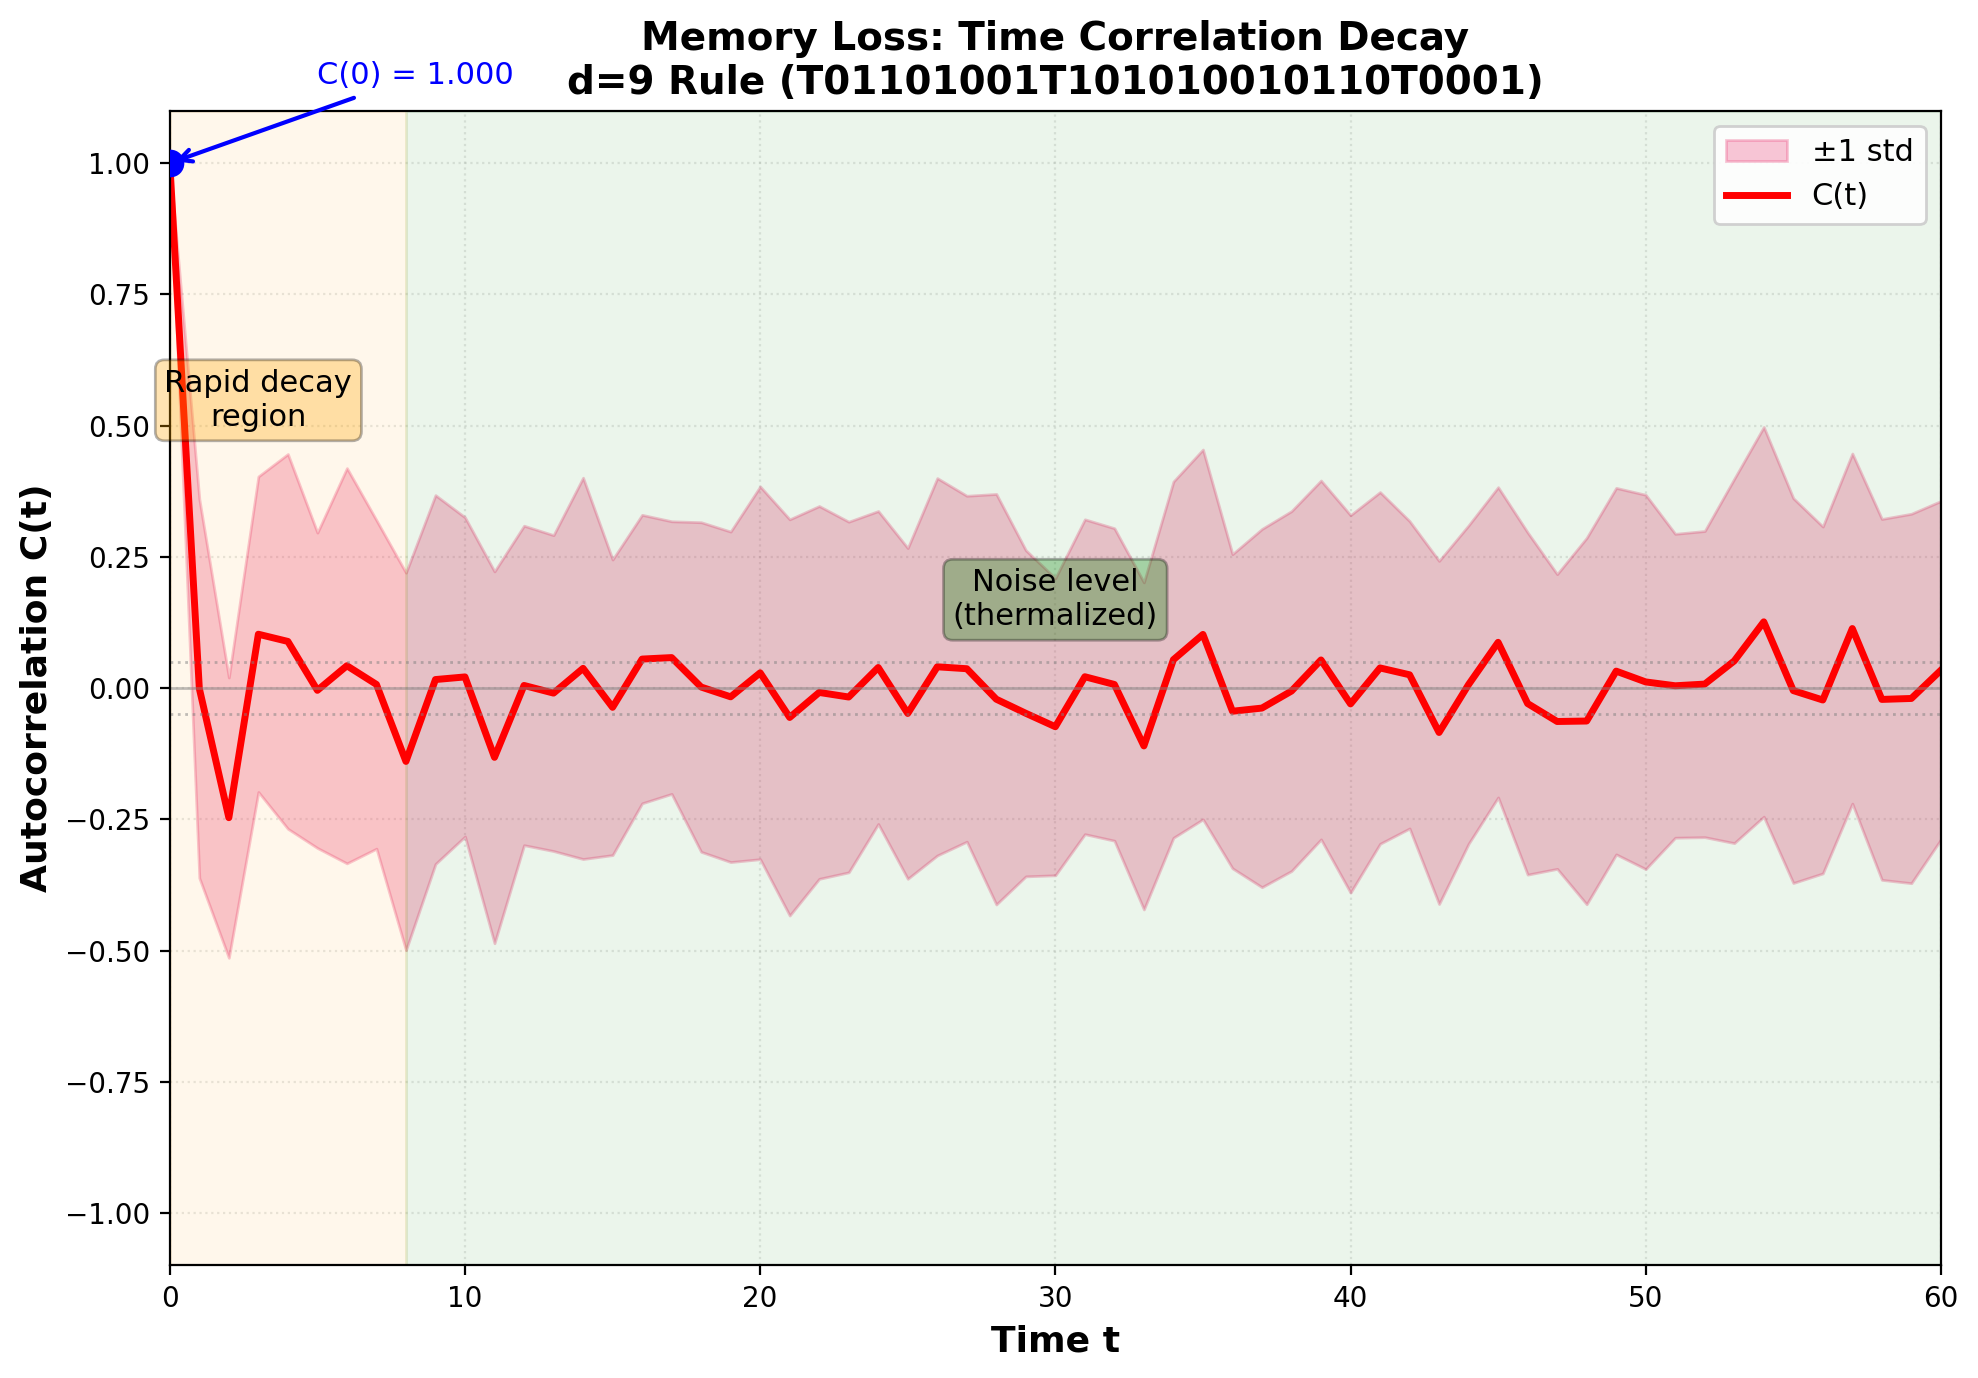
\includegraphics[width=0.45\textwidth]{image/2_memory_loss.png} 
\caption{\label{d9_memory}d=9时，体系在长期上衰减到零，并发生小幅波动，记忆丢失。}
\end{figure}

\begin{figure}[H]
\centering
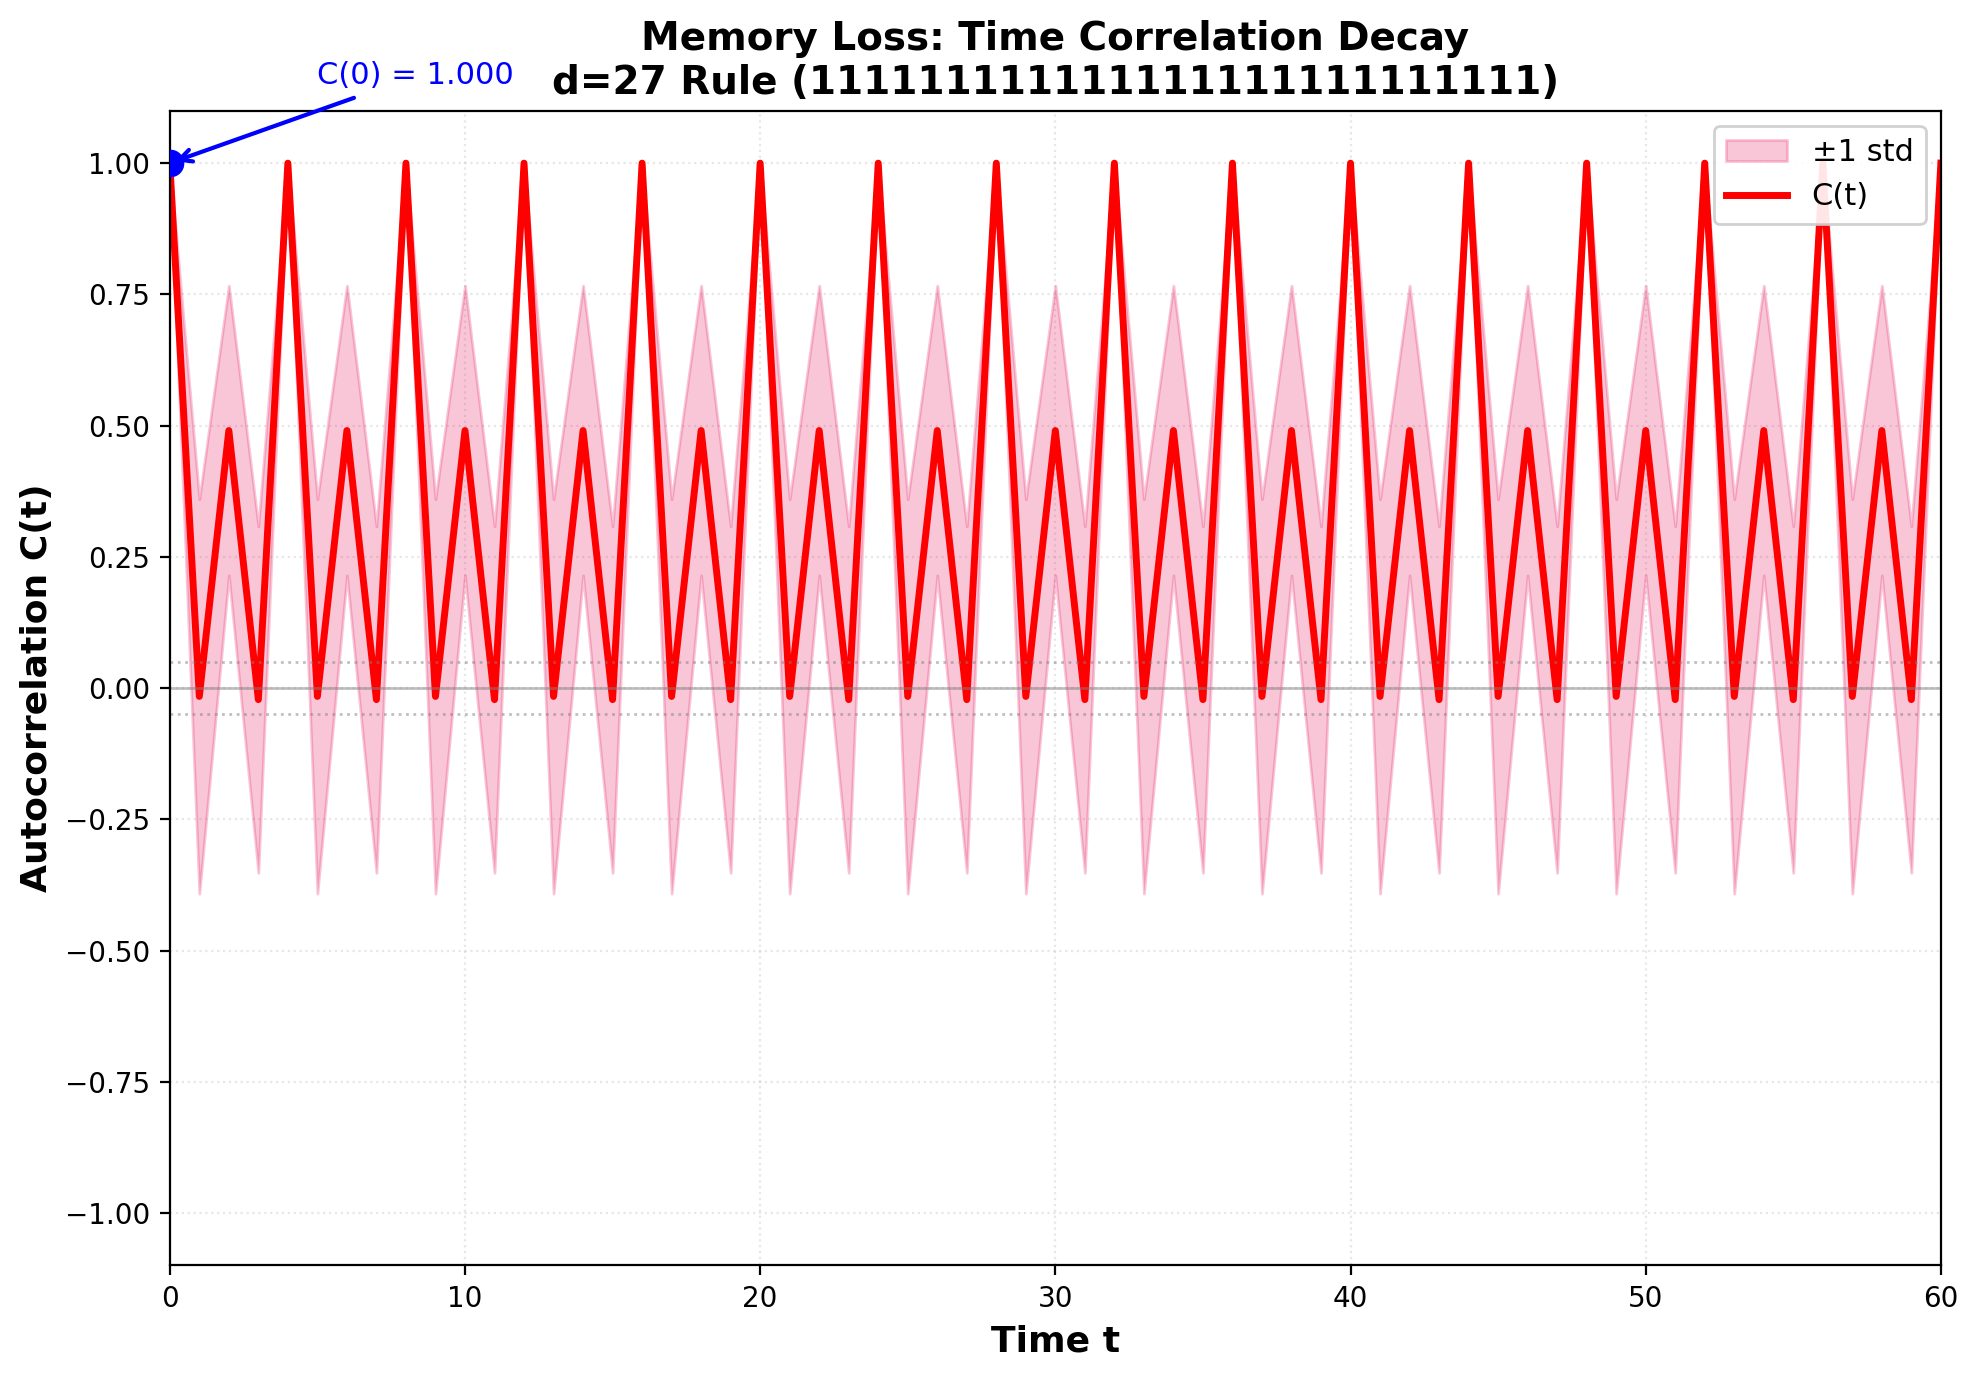
\includegraphics[width=0.45\textwidth]{image/2_memory_loss_new.png} 
\caption{\label{d27_memory}d=27时，体系在长期上以周期 4 振荡，不衰减，保存原有记忆。}
\end{figure}

如图\ref{d9_memory},\ref{d27_memory}，在$L=10$时，时间关联函数$C(t)$在$t \approx 5$时从$C(0)=1$快速衰减到$|C(t)| < 0.1$，随后围绕零小幅波动（幅度$\sim 0.05$）。
d=27规则的$C(t)$呈严格的周期4振荡：$C(t) = (0.62, 0.04, 0.32, 0.62, \ldots)$。
这表明时间关联函数是验证热化行为的重要辅助指标。热化系统的C(t) 会快速衰减到零，而非热化系统则保持周期振荡或缓慢衰减。

为了分析体系在长时间演化后的行为，我们定义关联饱和值：
\begin{equation}
    C_{sat} = \frac{1}{20} \sum_{T-19}^{T} |C(t)|\text{ （体系演化最后20步的$|C(t)|$）}
\end{equation}

\begin{figure}[H]
\centering
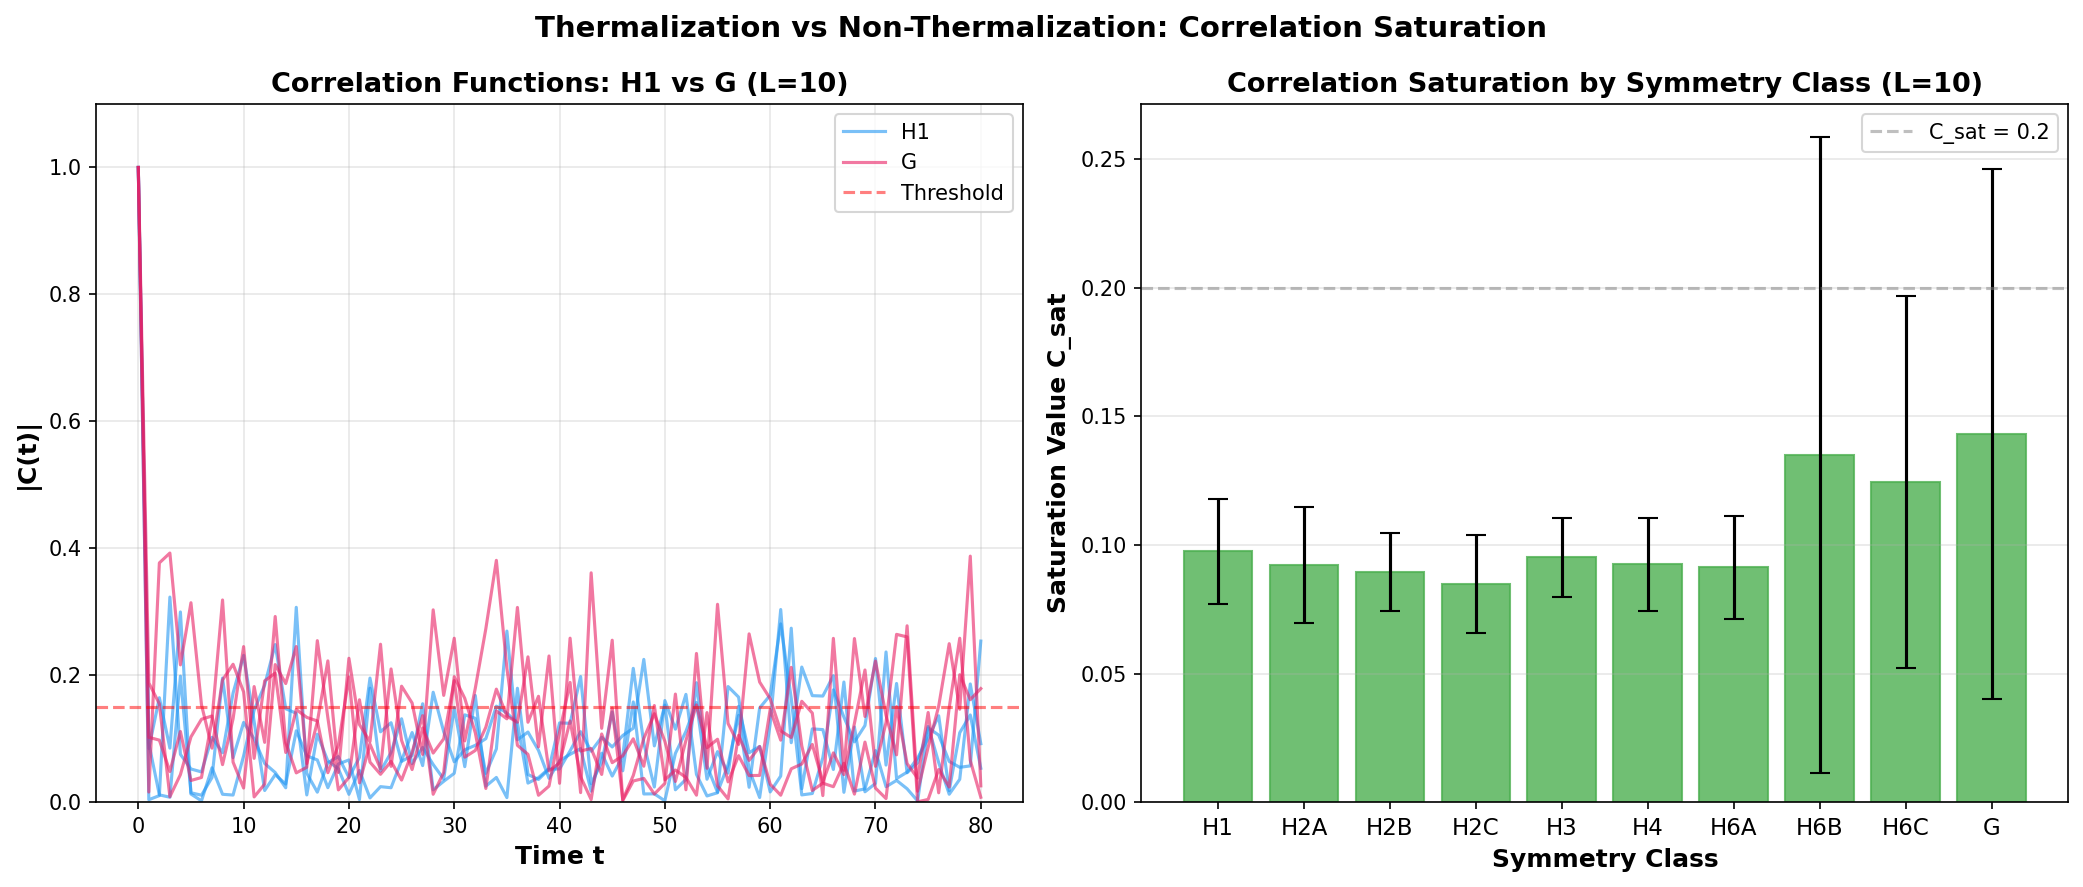
\includegraphics[width=0.45\textwidth]{image/correlation_saturation.png} 
\caption{\label{correlation_saturation}左图：$G$和$H_1$的$C(t)$变化；右图：各个种类$C_{sat}$的值。}
\end{figure}
如图\ref{correlation_saturation}，非热化规则的$C_{sat}$也可以接近零（0.08-0.11），看起来像"热化"了。但结合 d 值和轨道分析，它们实际上是被守恒量约束在低维子流形上，并未真正遍历整个相空间。
因此，关联衰减是热化的必要但不充分条件。

我们想寻找C(t)是否满足：
\begin{equation}
    C(t) \sim e^{-\gamma t}
\end{equation}
但我们经过对15个$d=9$规则的关联衰减指数$\gamma$（通过拟合得到）的统计显示均值为0.14，变异系数为0.73，不具有普适性，如图\ref{correlation_gamma},\ref{correlation_decay}所示。
$\gamma$同样依赖于$f$的微观选取。并不是一个普适量。

\begin{figure}[H]
\centering
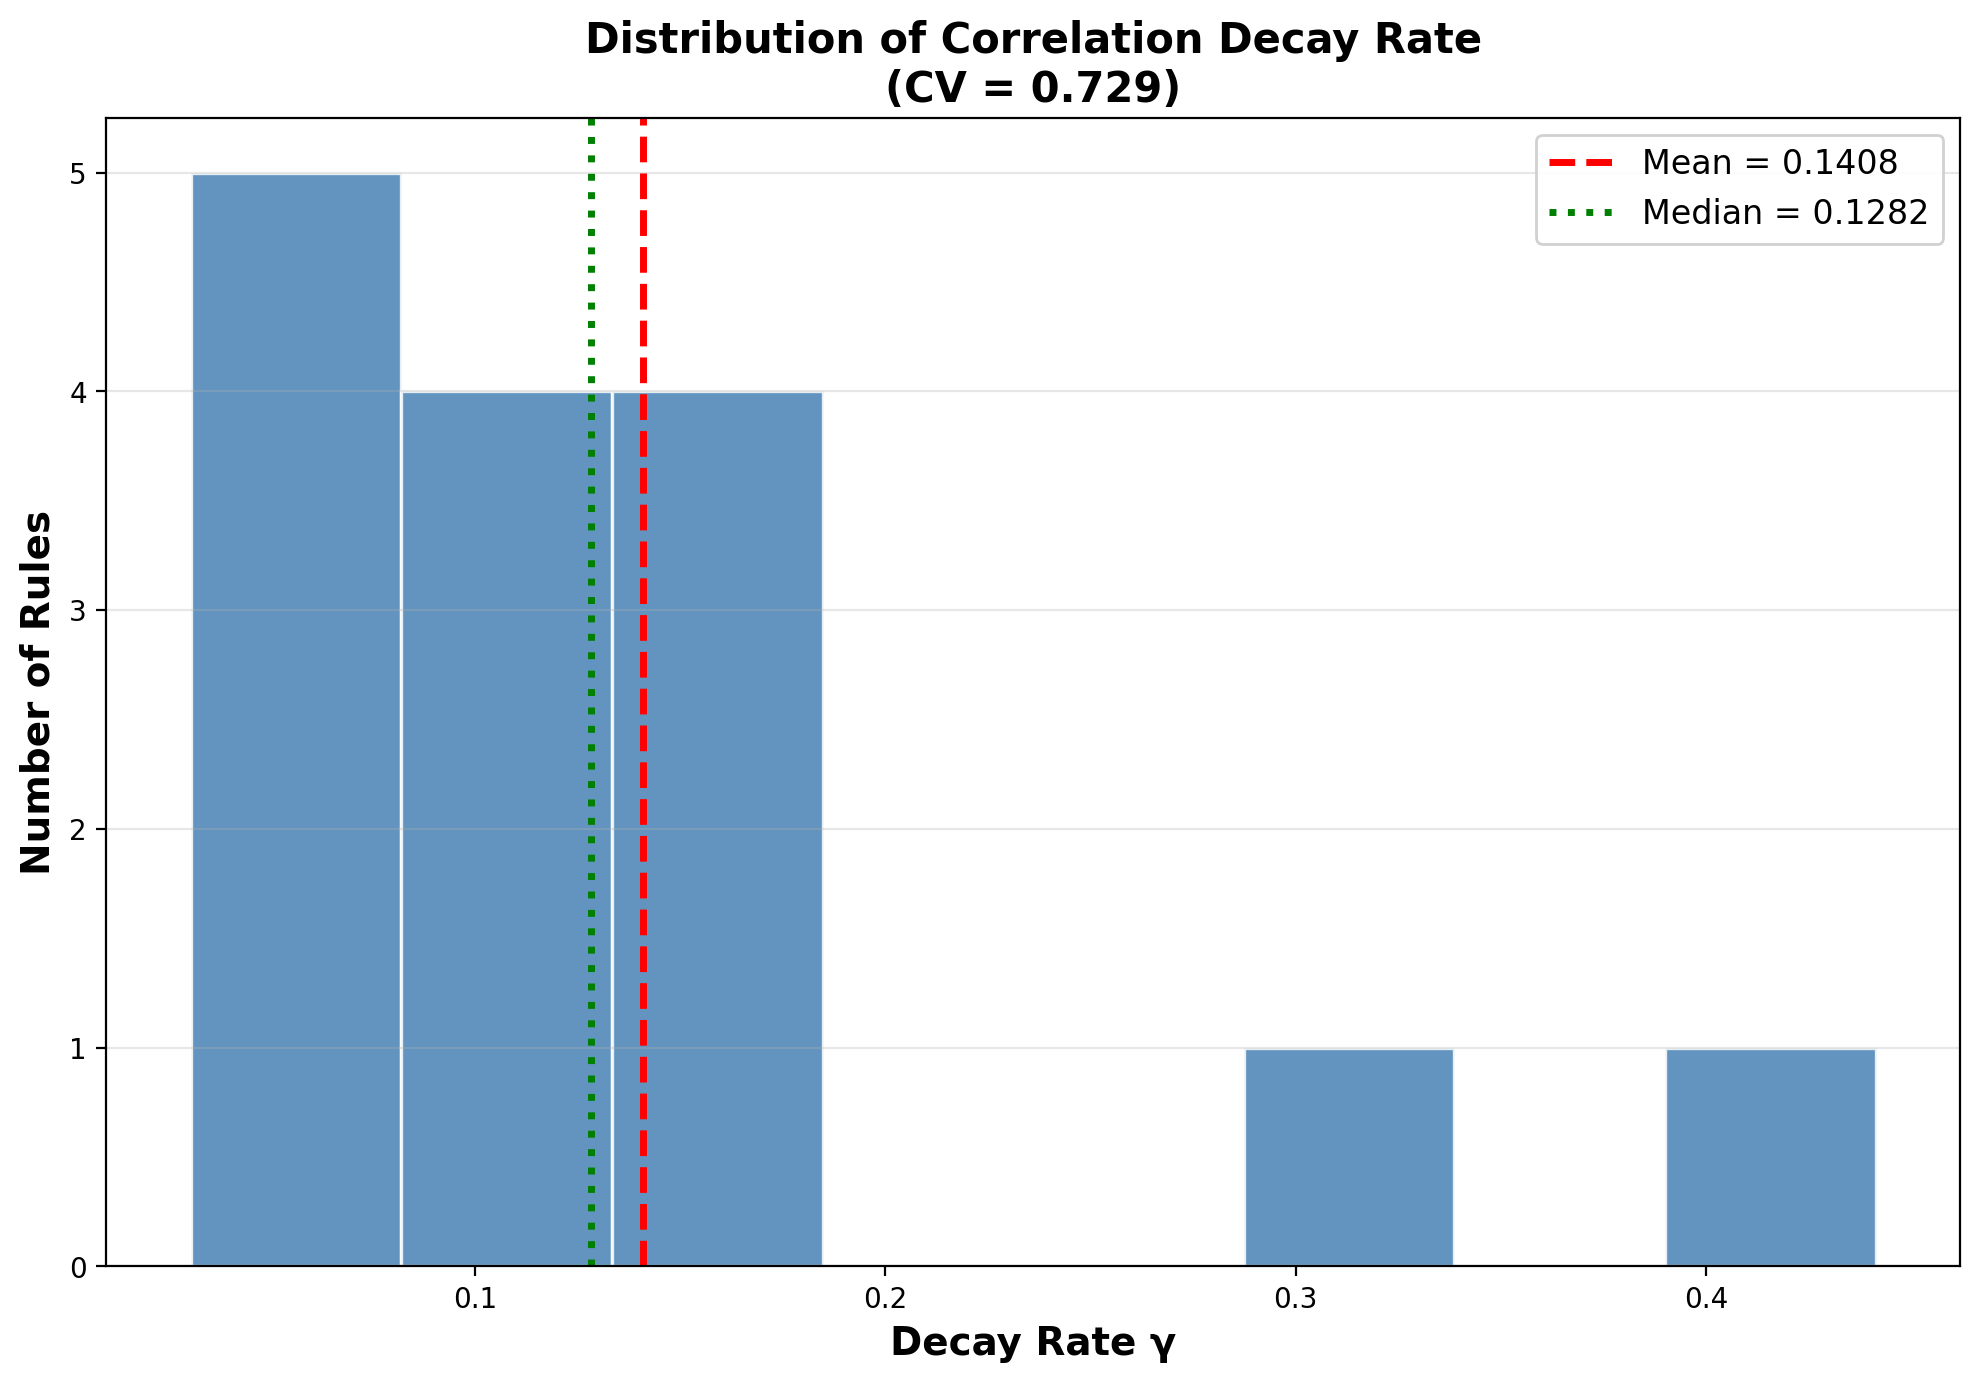
\includegraphics[width=0.45\textwidth]{image/fig_gamma_histogram.png} 
\caption{\label{correlation_gamma}$\gamma$不存在普适性。}
\end{figure}

\begin{figure}[H]
\centering
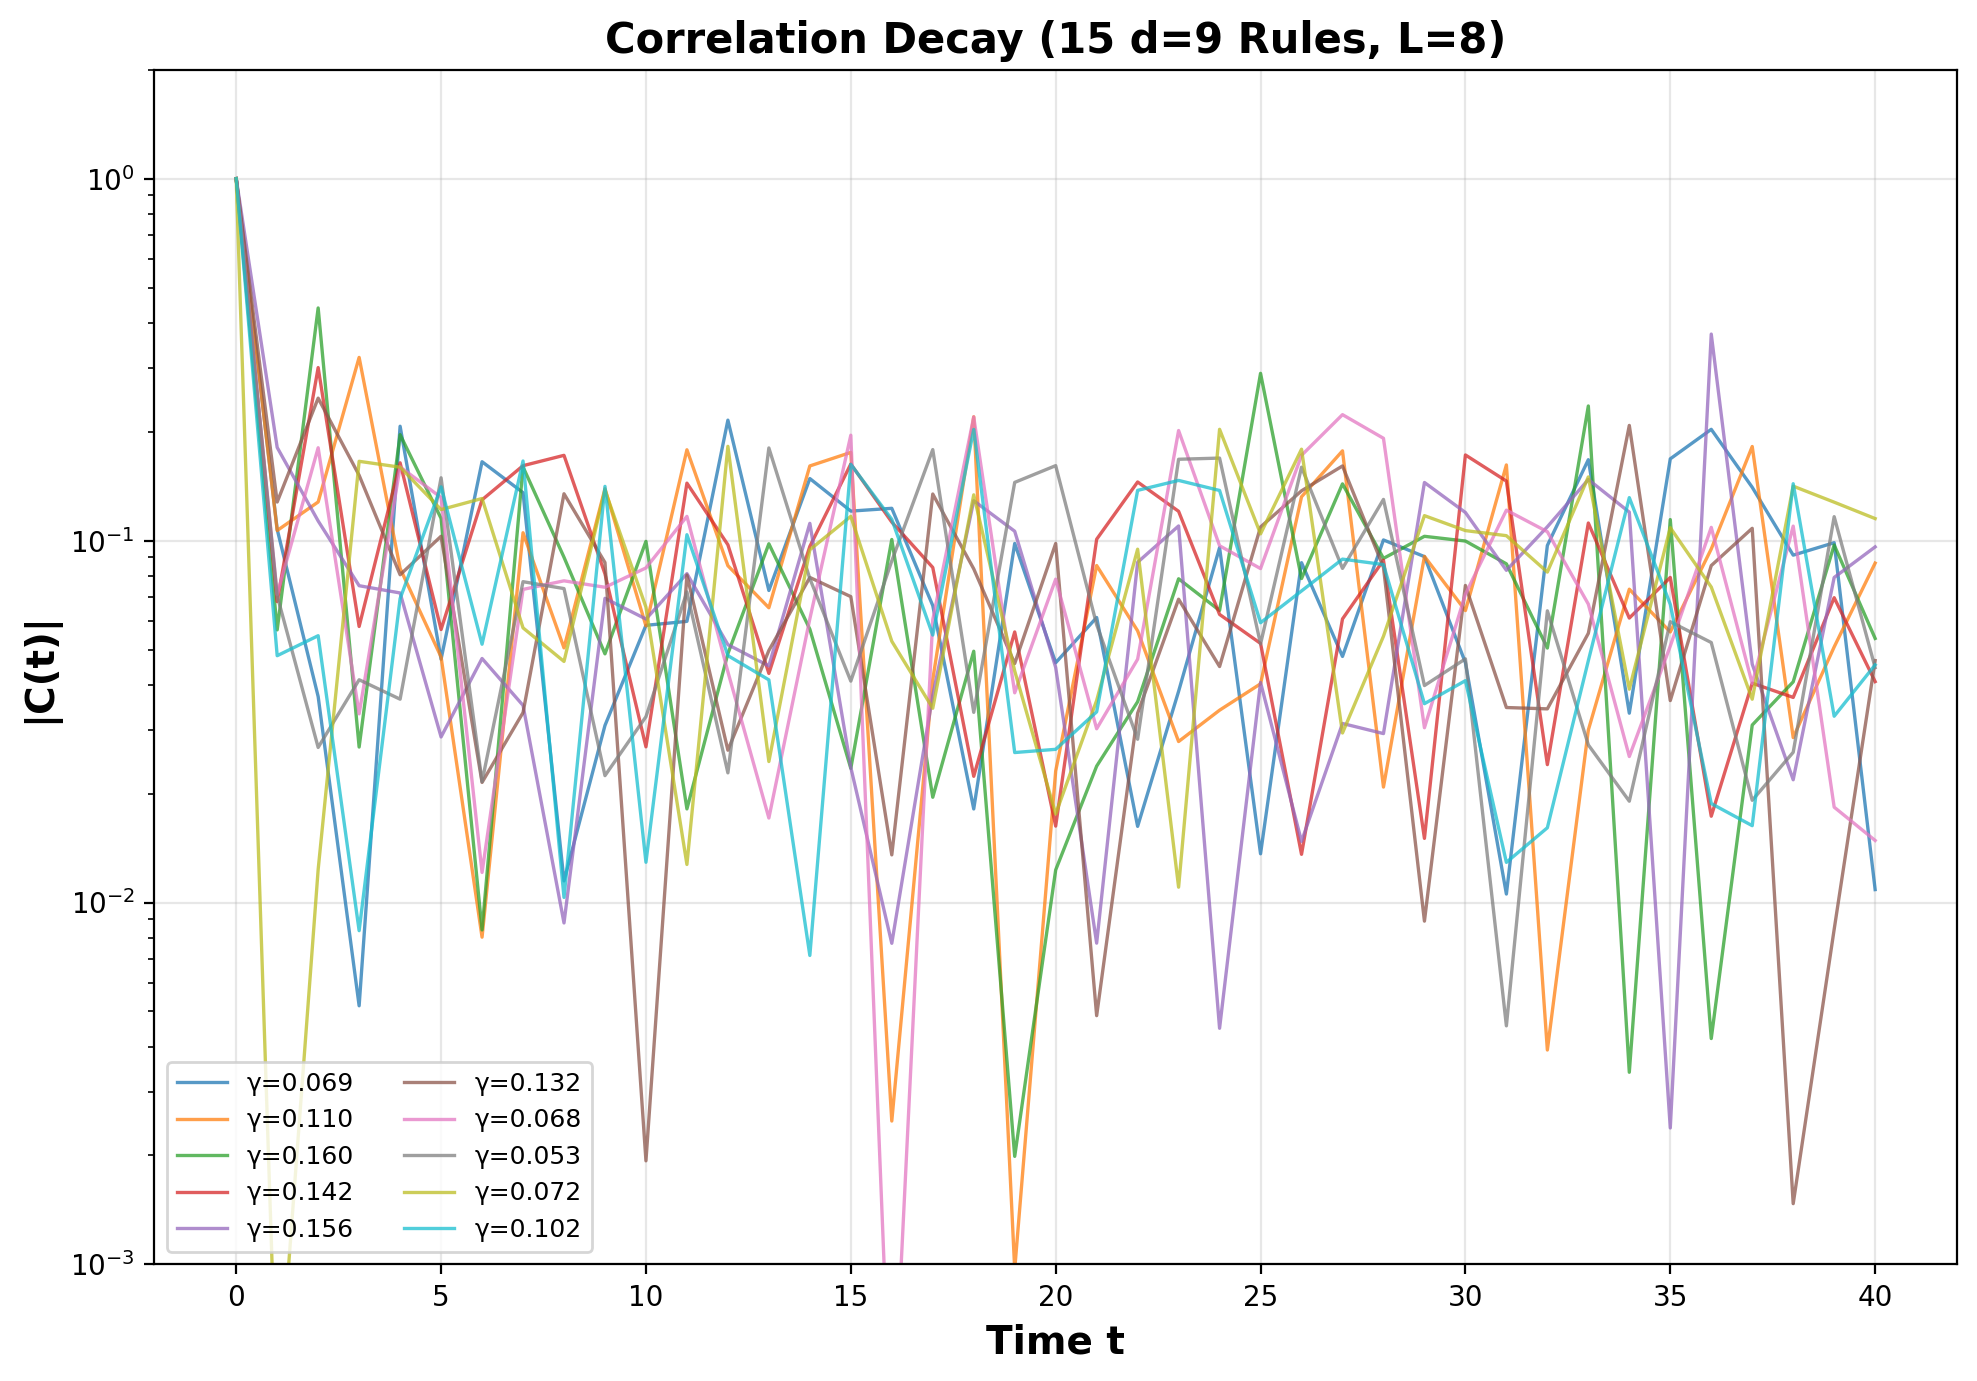
\includegraphics[width=0.45\textwidth]{image/fig_correlation_decay.png} 
\caption{\label{correlation_decay}$d=9$的15个$f$的关联函数演化。}
\end{figure}

\subsubsection{Feigenbaum常数搜索}
为了验证体系是否是直接混动，我们仿照$Feigenbaum$的方法，尝试了以下两种参数化方法寻找倍周期分岔\cite{Mitchell}：
\begin{itemize}
    \item 参数化$f$规则（在周期规则和混沌规则之间插值）:$$f_\lambda = ((1-\lambda)f_{periodic} + \lambda f_{chaotic})$$
    取最接近的{-1,0,1}
    \item 参数化$\otimes$表（在Rule 1和Rule 3间旋转（见图\ref{fig:ternary_operators}））。
\end{itemize}


但是两种方法均未观察到标准的倍周期分岔序列。在参数化$f$的扫描中，估算的$\delta$值为$-0.004$和$2.44$，与Feigenbaum常数$\delta = 4.669$相差甚远。
$delta$为负可能是由于有限分辨率导致的伪迹或参数化方向。这表明三元ERCA的混沌不是通过$Feigenbaum$型倍周期分岔产生的，而是规则空间中直接存在的混沌。这与我们之前的分析一致。

\subsubsection{讨论}
在结束这一部分之前，我们想对某些问题进行说明：
\begin{itemize}
    \item 所有规则（包括非热化规则）的Lyapunov指数都为正，时间关联都可以衰减，表明混沌普遍存在。然而，混沌不等同于热化：非热化规则虽然表现出混沌行为，但由于额外守恒量的约束，轨道被限制在相空间的低维子流形上。这体现在轨道长度上——热化类的轨道长度系统性地大于非热化类，且两者差距在$L$增大时扩大。这一区分揭示了可加性守恒量判据的独特价值：Lyapunov指数和关联衰减不能区分热化和非热化（两者在非热化规则中也成立），而$d=9$是唯一可靠的二分判据。
    \item 三轮换对称性不通过Noether定理产生守恒量（因为它是离散对称性），而是通过约束$f$在定义域轨道上的取值来强制产生可加性守恒量。在$G$作用下，定义域有6个轨道。三轮换对称性要求$f$在这些轨道上取特定关系，这些约束导致$M_f$的秩从72（d=9）降低到54-68（d=11-27），从而产生额外的零空间方向。
    \item 本研究区分了普适和非普适的性质。普适的性质包括：$d=9 \iff$热化的定性判据、$\lambda > 0$的存在性（100\%的规则）、$\lambda$的Gaussian分布形态（KS检验$p=0.97$）、$\lambda_\infty > 0$的热力学极限行为。非普适的性质包括：轨道长度指数$\alpha$（变异系数0.64）、关联衰减指数$\gamma$（变异系数0.73）、$\lambda$的具体数值。这类似于统计力学中临界指数是普适的而临界温度不是\cite{Yakov}。
\end{itemize}

\begin{figure}[H]
\centering
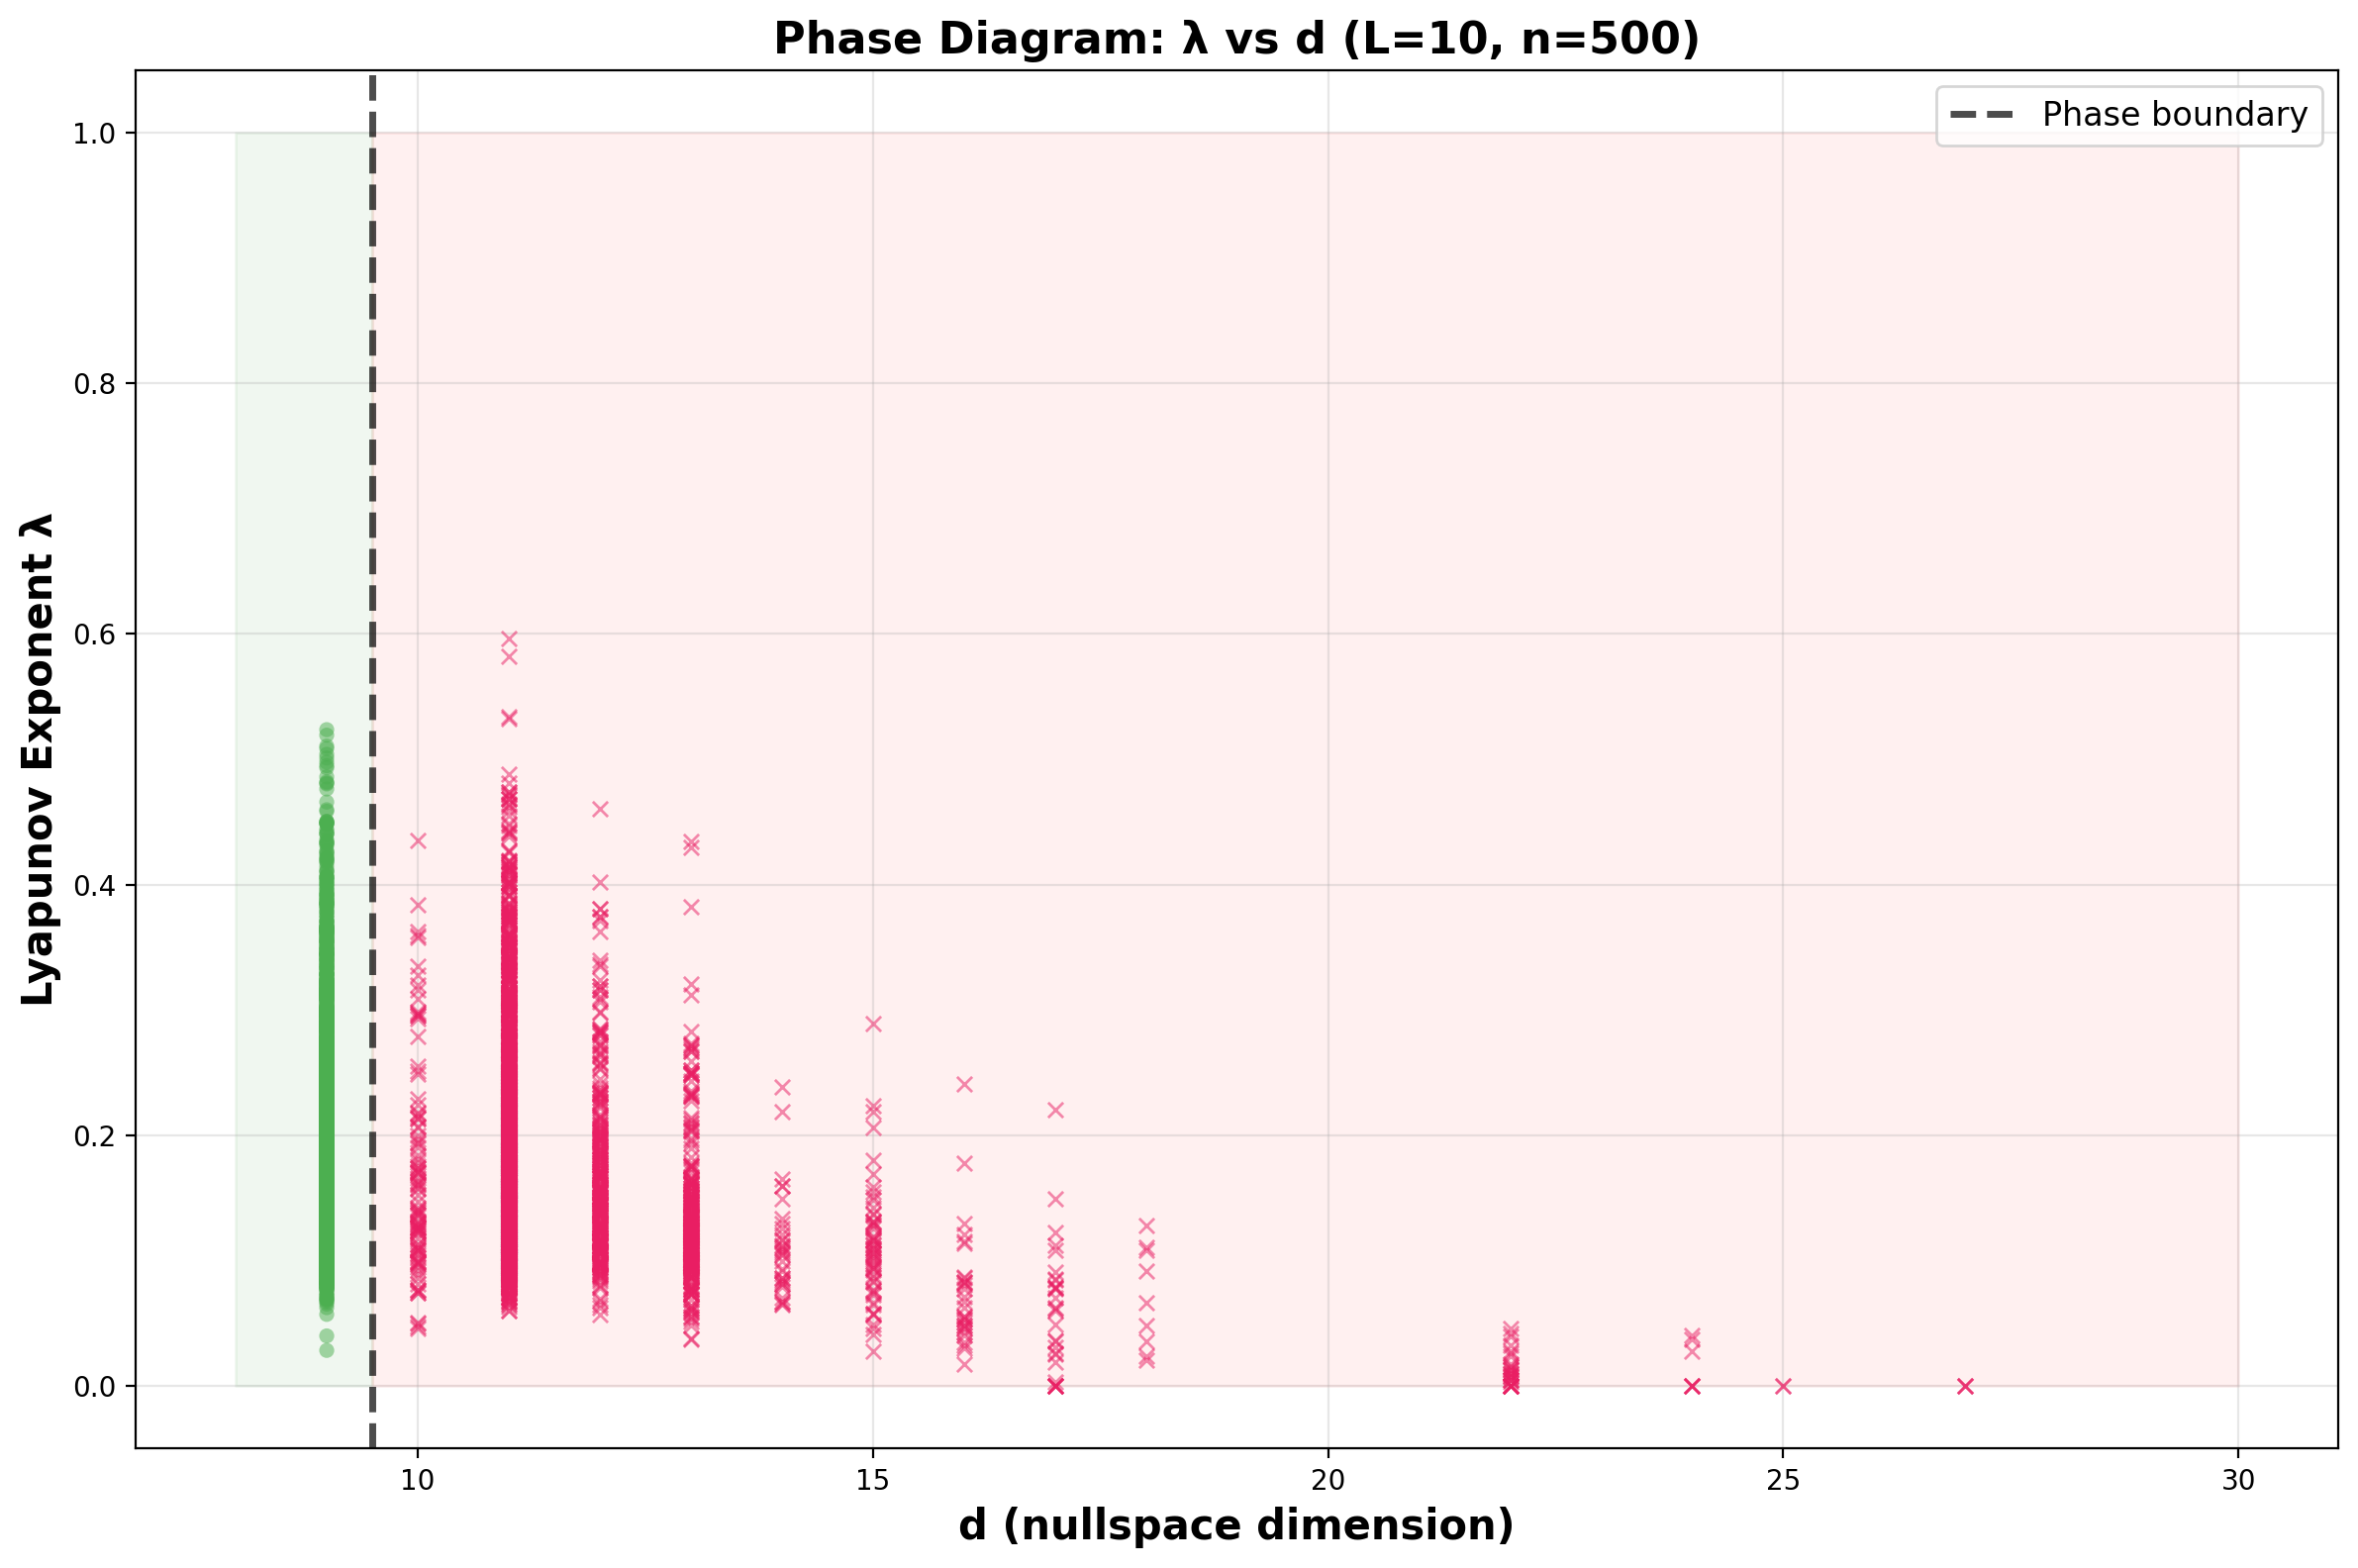
\includegraphics[width=0.45\textwidth]{image/fig4_lambda_vs_d.png} 
\caption{$\lambda$和$d$之间的相图，绿色圆点为热化规则（$d=9$），红色叉号为非热化规则（$d>9$）。黑色虚线标记相边界$d=9.5$。}
\end{figure}

\begin{figure}[H]
\centering
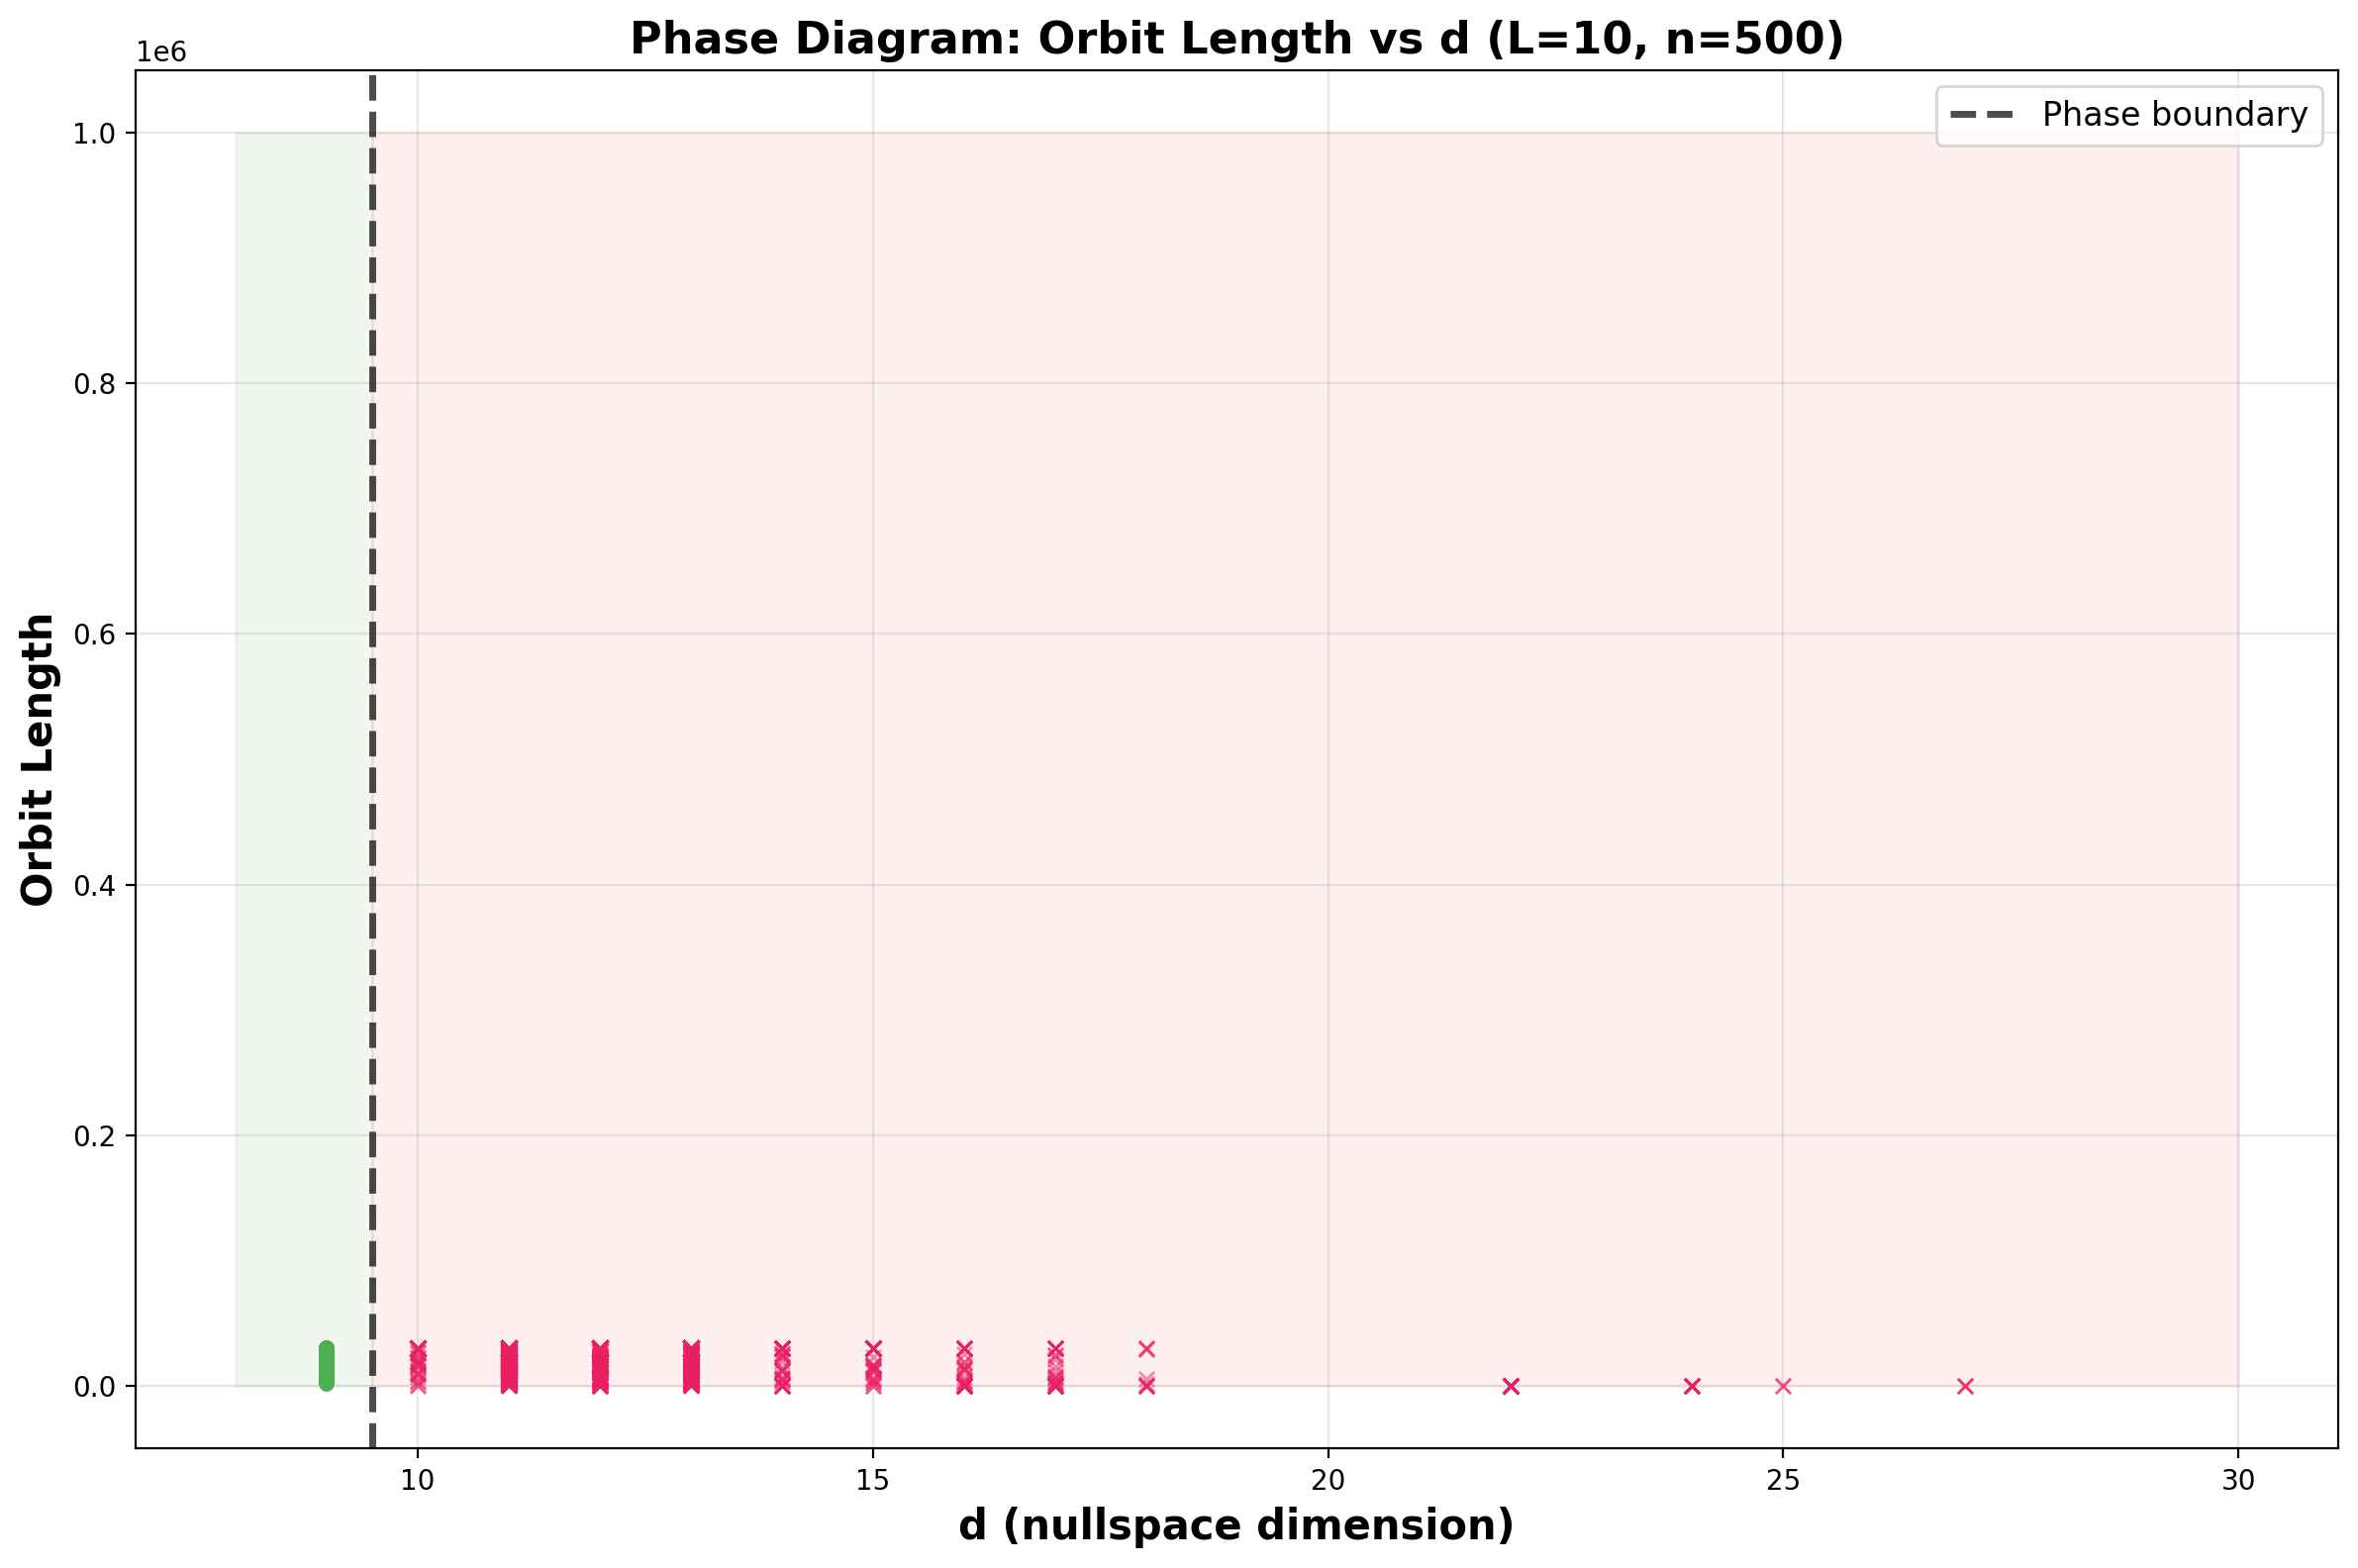
\includegraphics[width=0.45\textwidth]{image/fig5_orbit_vs_d.png} 
\caption{轨道长度和$d$之间的相图。}
\end{figure}

\begin{figure}[H]
\centering
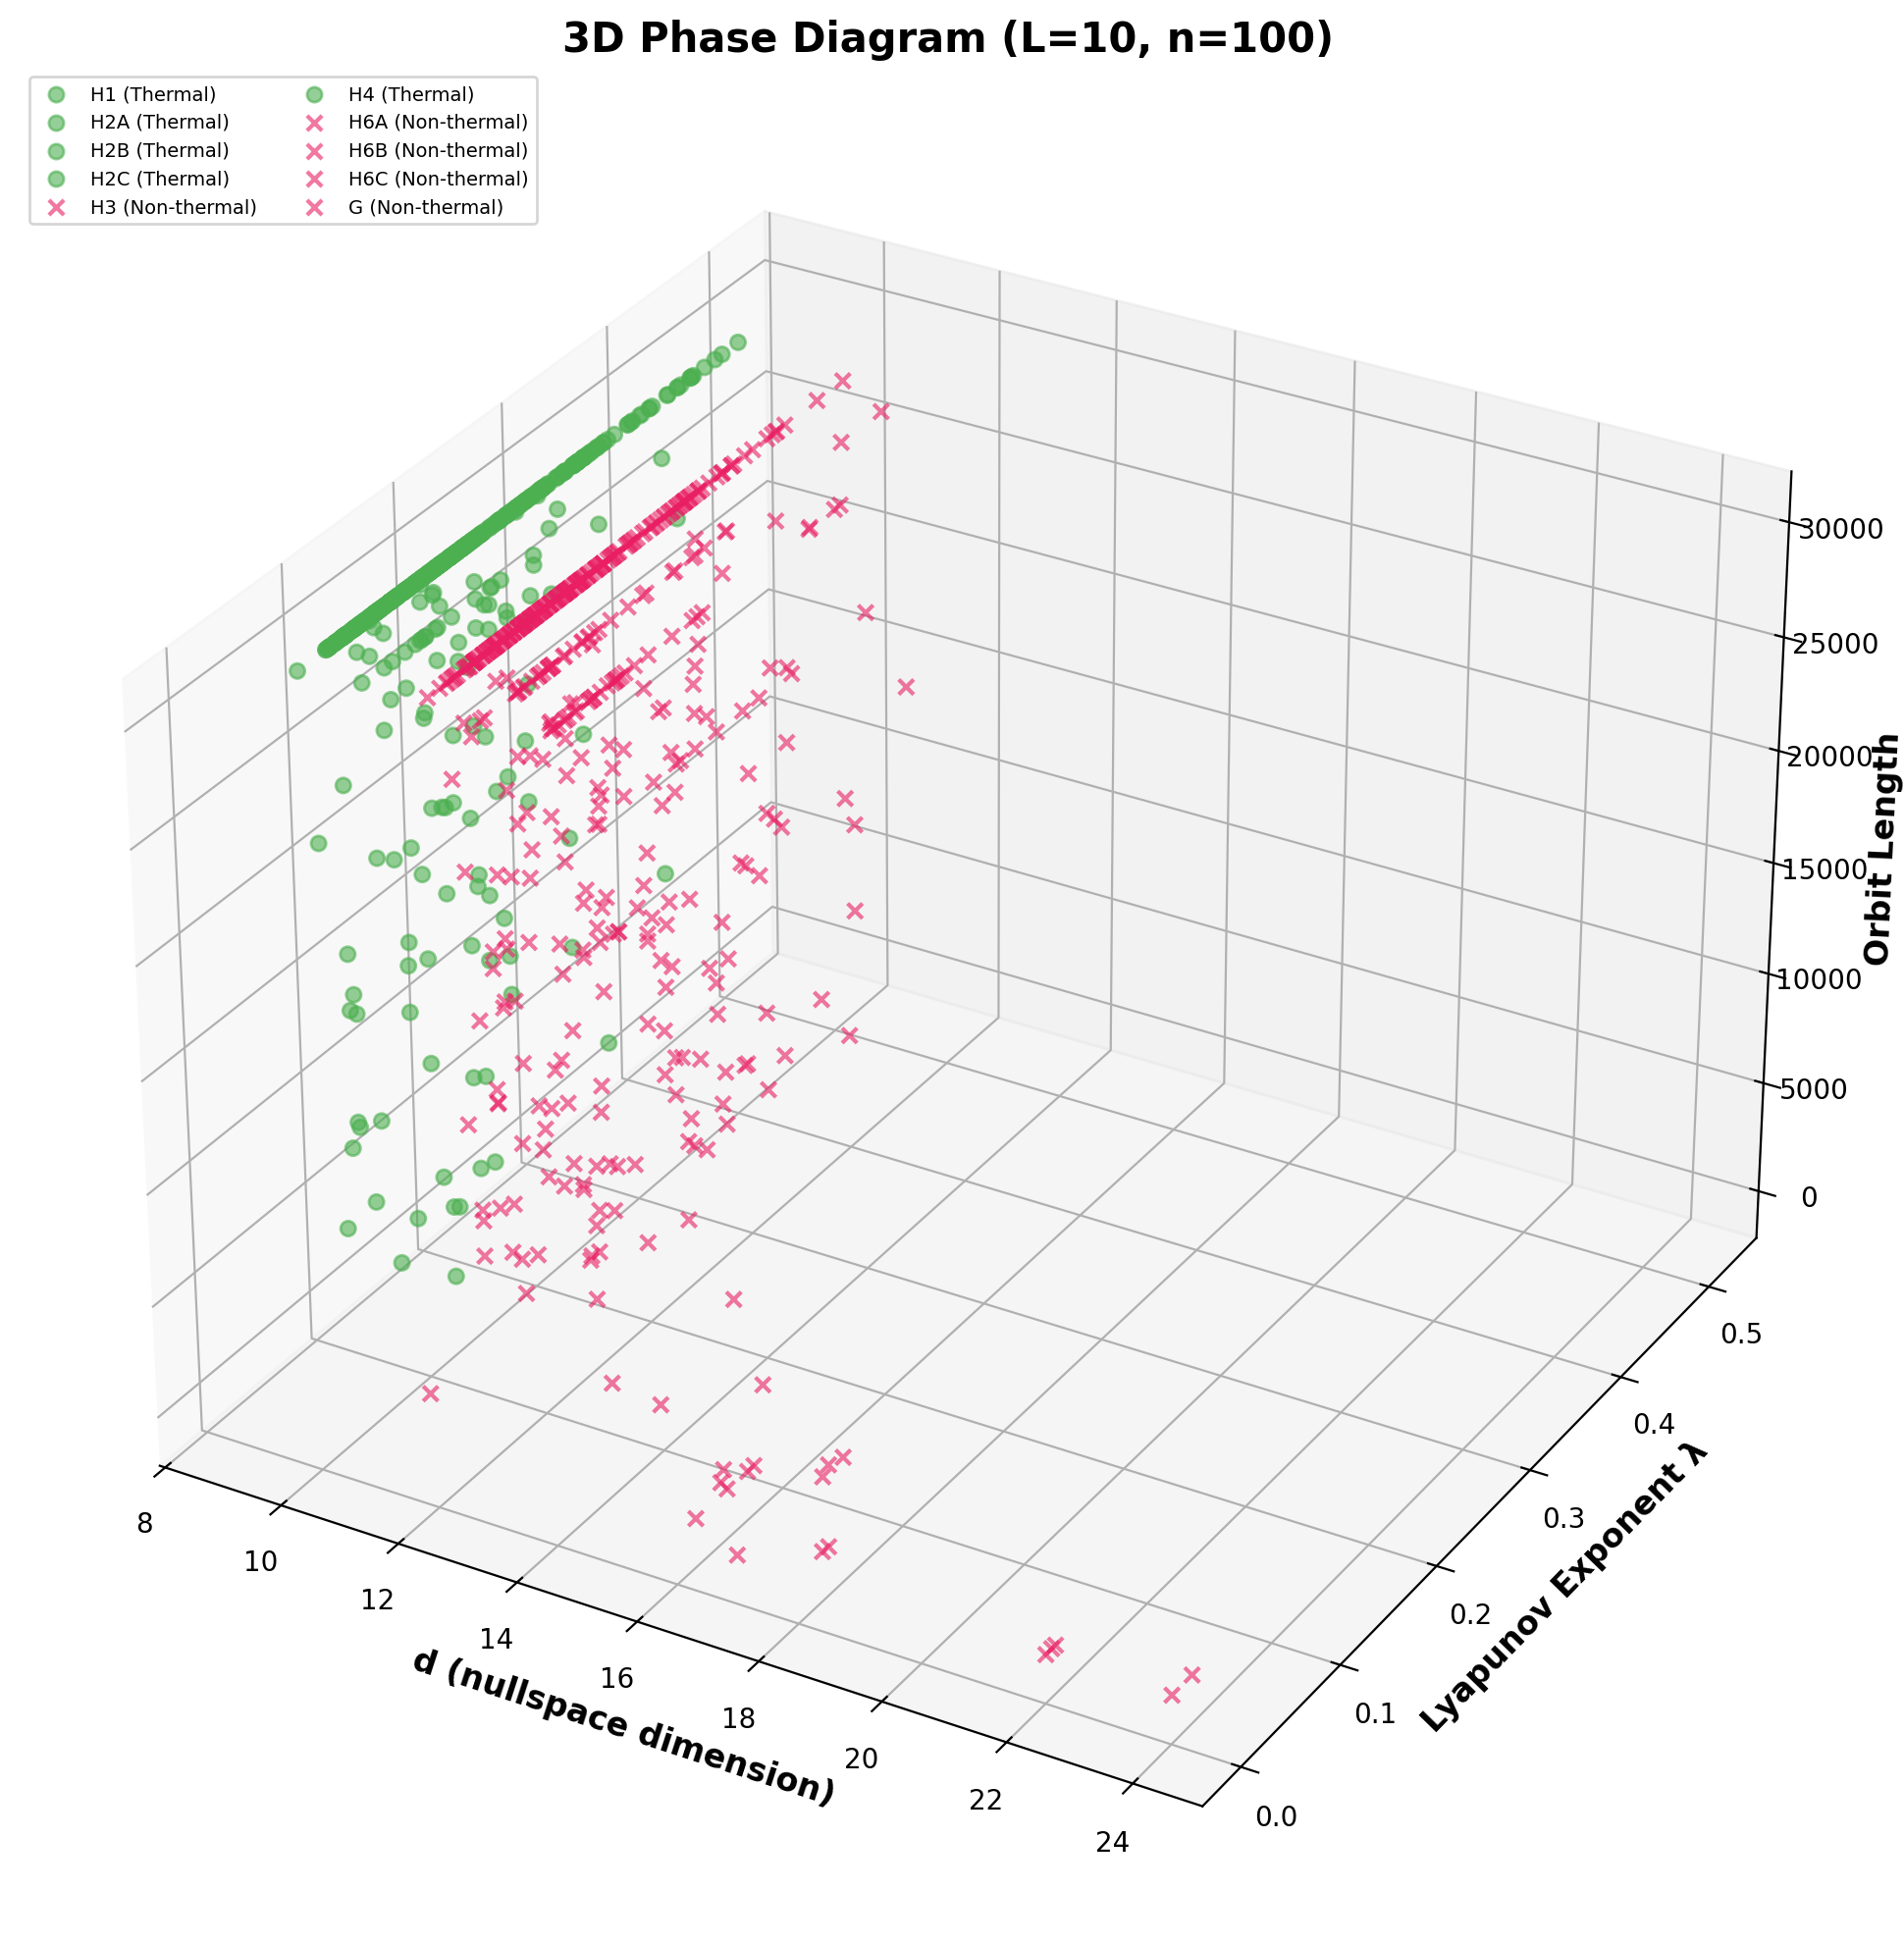
\includegraphics[width=0.45\textwidth]{image/fig6_3d_phase_diagram.png} 
\caption{三维相图：$(d, \lambda, \text{轨道长度})$。热化规则（绿色圆点）聚集在$d=9$平面附近。非热化规则（红色叉号）分布在$d>9$区域。}
\end{figure}

\FloatBarrier
\section{结论}

本文基于 Shinji Takesue 的经典分析框架，探讨了确定性可逆元胞自动机（RCA）的相空间拓扑结构与动力学遍历特征。

研究主要分为两个层面：首先，通过对二进制 ERCA 的复现与分析，我们验证了局域演化规则对相空间流形的非对称分割作用。研究发现，线性加性规则因存在局域守恒墙而呈现出较强的非遍历性与数论相关的奇异周期；而非线性混沌规则由于不存在此类几何限制，表现出相空间轨道的指数级发散，从而在动力学层面具备了统计混合特征。
其次，我们将系统状态空间成功扩展至三值（$\{-1, 0, 1\}$）离散流形。该扩展不仅增加了模型的自由度，更为精细化控制微观轨线在相空间中的运动轨迹提供了数理依据。我们认为，这种新的相空间具有丰富得多的性质，有着广泛的研究前景。
综上所述，本课题通过构建不同规则下的离散流形图谱，定量化地展示了微观演化规则如何通过相空间几何剪裁，直接影响系统的遍历行为，为理解确定性系统如何从微观层面涌现出宏观统计特性提供了参考。

\bibliography{cite}

\appendix

\section{三元ERCA规则表述方法}
在三元ERCA中，我们难以再使用二元ERCA中常用的八位二进制数来表述规则。我们可以使用
一个$3^3$位的三进制数来表述f规则。例如规则$T010011TT0TT0TT0T111T10T101$，($T$代表$-1$)对于$f(\mu,\nu,\kappa)$的
各个输入值的输出值如下表所示：
\begin{table}[ht]
\caption{\label{tab:ternary_rule} 规则 $T01 001 1TT 0TT 0TT 0T1 11T 10T 101$ 的输入输出关系表}
\begin{ruledtabular}
\begin{tabular}{cccc}
输入 $\mu$ & 输入 $\nu$ & 输入 $\kappa$ & 输出 $f(\mu,\nu,\kappa)$ \\
\colrule
$1$ & $1$ & $1$ & $-1$ \\
$1$ & $1$ & $0$ & $0$ \\
$1$ & $1$ & $-1$ & $1$ \\
$1$ & $0$ & $1$ & $0$ \\
$1$ & $0$ & $0$ & $0$ \\
$1$ & $0$ & $-1$ & $1$ \\
$1$ & $-1$ & $1$ & $1$ \\
$1$ & $-1$ & $0$ & $-1$ \\
$1$ & $-1$ & $-1$ & $-1$ \\
$0$ & $1$ & $1$ & $0$ \\
$0$ & $1$ & $0$ & $-1$ \\
$0$ & $1$ & $-1$ & $-1$ \\
$0$ & $0$ & $1$ & $0$ \\
$0$ & $0$ & $0$ & $-1$ \\
$0$ & $0$ & $-1$ & $-1$ \\
$0$ & $-1$ & $1$ & $0$ \\
$0$ & $-1$ & $0$ & $-1$ \\
$0$ & $-1$ & $-1$ & $1$ \\
$-1$ & $1$ & $1$ & $1$ \\
$-1$ & $1$ & $0$ & $1$ \\
$-1$ & $1$ & $-1$ & $-1$ \\
$-1$ & $0$ & $1$ & $1$ \\
$-1$ & $0$ & $0$ & $0$ \\
$-1$ & $0$ & $-1$ & $-1$ \\
$-1$ & $-1$ & $1$ & $1$ \\
$-1$ & $-1$ & $0$ & $0$ \\
$-1$ & $-1$ & $-1$ & $1$ \\
\end{tabular}
\end{ruledtabular}
\end{table}

我们将在本篇文章中使用如$T010011TT0TT0TT0T111T10T101$类似的方式标注三元ERCA的$3^{27}$条规则。

\section{各人评分}
\begin{itemize}
    \item Q. Tan，三值ERCA的主要内容与论文整体建构，50/100
    \item Z. Yang， 二元遍历假说验证及论文初稿部分，50/100
\end{itemize}

\end{document}
